\documentclass[11pt,a4paper]{article}
\usepackage[utf8]{inputenc}
\usepackage[T1]{fontenc}
\usepackage{geometry}
\usepackage{hyperref}
\usepackage{graphicx}
\usepackage{amsmath}
\usepackage{amsfonts}
\usepackage{amssymb}
\usepackage{xcolor}
\usepackage{listings}
\usepackage{titlesec}
\usepackage{longtable}
\usepackage{fancyhdr}
\usepackage{enumitem}
\renewcommand{\raggedright}{\justifying}
\setlength{\baselineskip}{1.5\baselineskip} % Fixed: was 1.5in (too large)

% Page layout
\geometry{margin=1in}

% Hyperlink setup
\hypersetup{
    colorlinks=false,
    linkcolor=black,
    filecolor=magenta,      
    urlcolor=cyan,
    pdftitle={Documentation},
    pdfpagemode=FullScreen,
}

% Custom section formatting
\titleformat{\section}{\Large\bfseries}{\thesection}{1em}{}
\titleformat{\subsection}{\large\bfseries}{\thesubsection}{1em}{}
\titleformat{\subsubsection}{\bfseries}{\thesubsubsection}{1em}{}

% Listings setup for code
\lstset{
    basicstyle=\ttfamily\small,
    breaklines=true,
    frame=single,
    numbers=left,
    numberstyle=\tiny,
    stepnumber=1,
    numbersep=5pt,
    showstringspaces=false,
    keywordstyle=\color{black},
    commentstyle=\color{gray},
    stringstyle=\color{red}
}

% Header and footer
\pagestyle{fancy}
\fancyhf{}
\fancyhead[L]{\leftmark}
\fancyhead[R]{\thepage}
\renewcommand{\headrulewidth}{0.4pt}
\setlength{\headheight}{14pt}

% Title page info
\title{Finance \& Accounting Manual}
\author{Axon System}
\date{\today}

\begin{document}

% Title page
\begin{titlepage}
    \centering
    \vspace*{2cm}
    {\Huge\bfseries Finance \& Accounting Manual\par}
    \vspace{1cm}
    {\Large Odoo Manual\par}
    \vspace{2cm}
    {\Large \textbf{Author:} Axon System\par}
    \vspace{0.5cm}
    {\Large \textbf{Date:} \today\par}
    \vfill
    
\includegraphics[width=0.3\textwidth]{logo.png}
    \vfill
\end{titlepage}

% Table of Contents
\tableofcontents
\newpage

% Main content starts here
\section{Introduction}
\subsection{Purpose of this Manual}
This manual is meant for leaders, trainers, and consultants working with financial management in Odoo. Its objectives are:

\begin{center}
    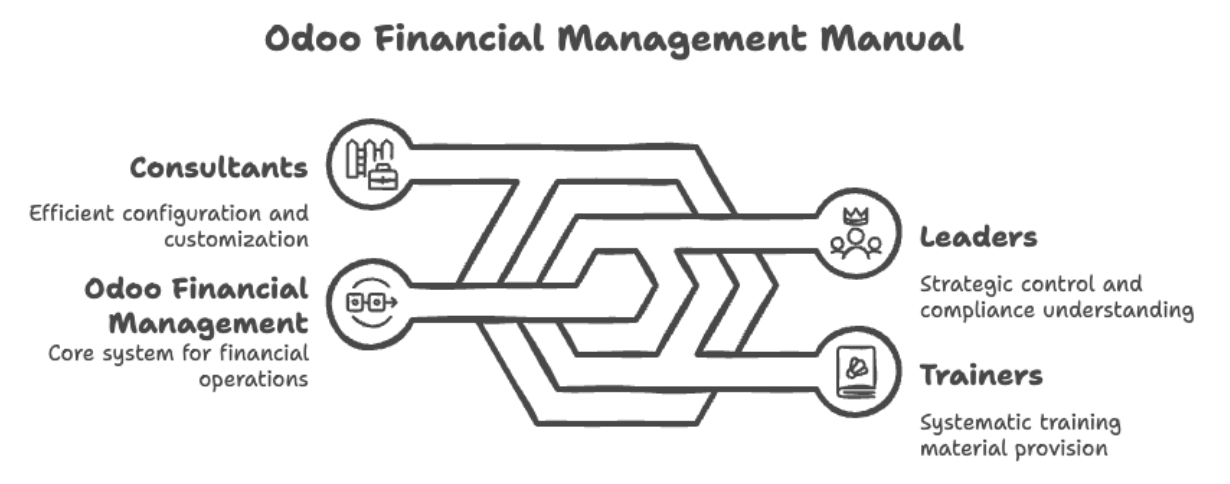
\includegraphics[width=0.8\linewidth]{diagram/odoo_financial_management_manual.png}
\end{center}

\noindent\textbf{Leaders:} To help you understand strategic financial control and compliance using Odoo.

\noindent\textbf{Trainers:} For the purpose of providing systematic material for training accountants.

\noindent\textbf{Consultants:} To enable efficient configuration, localization, and customization of Odoo for financial management.

\subsection{Enterprise Architecture Context}
This section describes the place of the Accounting module in the broader Odoo enterprise architecture and delineates the underlying technology stack that supports its functionality.
\bigskip

\noindent\textbf{Position of the Accounting Module}

\noindent The Accounting module is the fiscal backbone of the Odoo world. It brings together financial transactions and reporting, ensuring smooth fiscal control throughout departments. Thanks to its integration with several functional modules, it offers real-time financial visibility and control throughout the entire organization.
\bigskip

\noindent\textbf{Integration Points with Other Modules}

\noindent The Accounting module has strong integration points with some of the most significant Odoo modules, enabling end-to-end financial process automation:

\begin{center}
    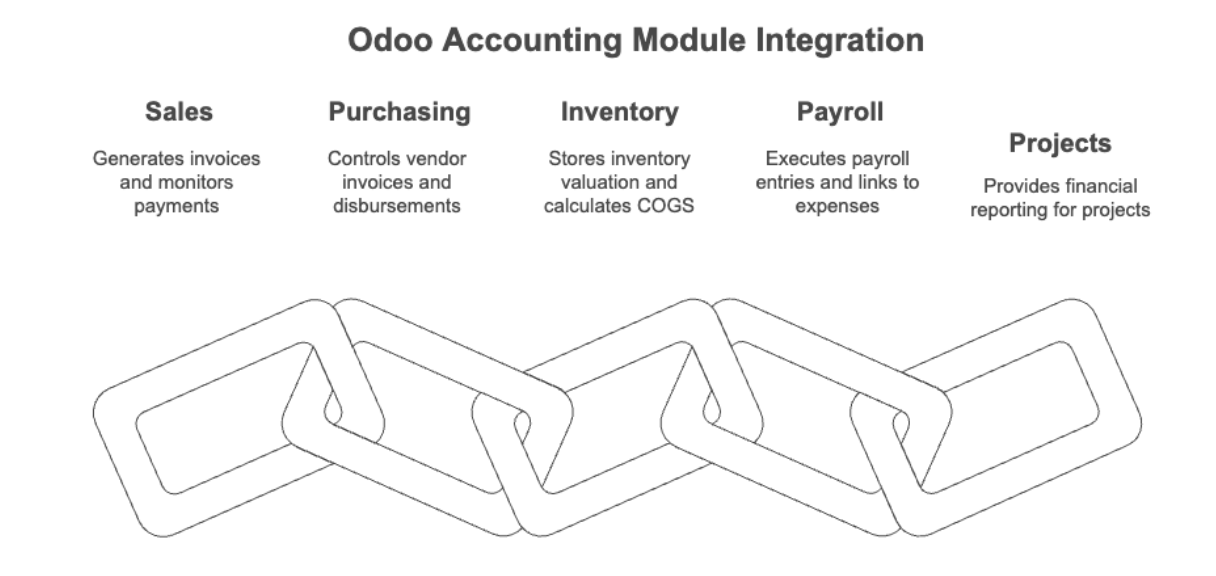
\includegraphics[width=0.8\linewidth]{diagram/odoo_accounting_module_integration.png}
\end{center}

\noindent\textbf{Sales:} Generates customer invoices automatically and monitors payment follow-ups.

\noindent\textbf{Purchasing:} Controls vendor invoices and disbursements going out.

\noindent\textbf{Inventory:} Stores inventory valuation in real time and on-the-fly calculation of COGS.

\noindent\textbf{Payroll:} Executes payroll journal entries and link to employee expense capture.

\noindent\textbf{Projects:} Provides financial reporting for project-level expense, revenue, and profitability.
\bigskip

\noindent\textbf{Technology Stack Overview}

\noindent Odoo's solid, modular design supports the Accounting module. Among the key constituents of the technology stack are:

\begin{center}
    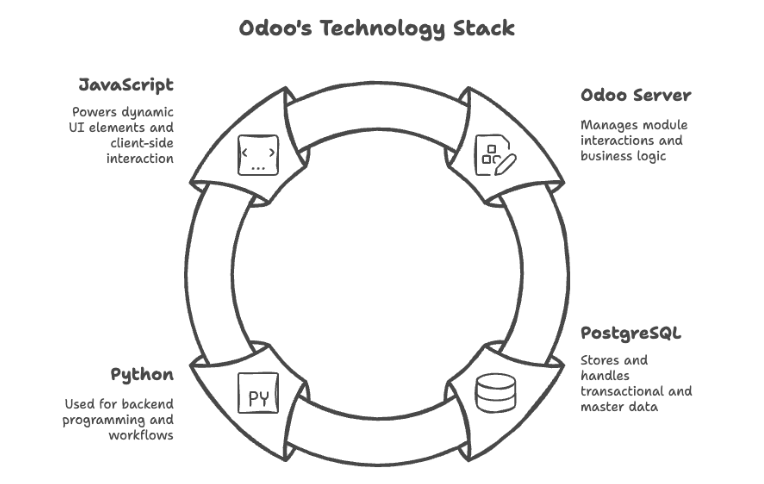
\includegraphics[width=0.8\linewidth]{diagram/odoo_technology_stack.png}
\end{center}

\noindent\textbf{Odoo Server:} The main framework that manages all module interactions and business logic.

\noindent\textbf{PostgreSQL:} A powerful open-source relational database management system used to store and handle transactional and master data.

\noindent\textbf{Python:} The primary backend programming language used for business logic coding and workflows.

\noindent\textbf{JavaScript (JS):} Used for dynamic user interface elements and client-side interaction within the web client.

\subsection{Supported Business Capabilities}
Odoo Accounting module provides organizations with an integrated suite of finance management capabilities, enabling effective, accurate, and compliant financial activities. Some of the key business capabilities are:

\begin{center}
    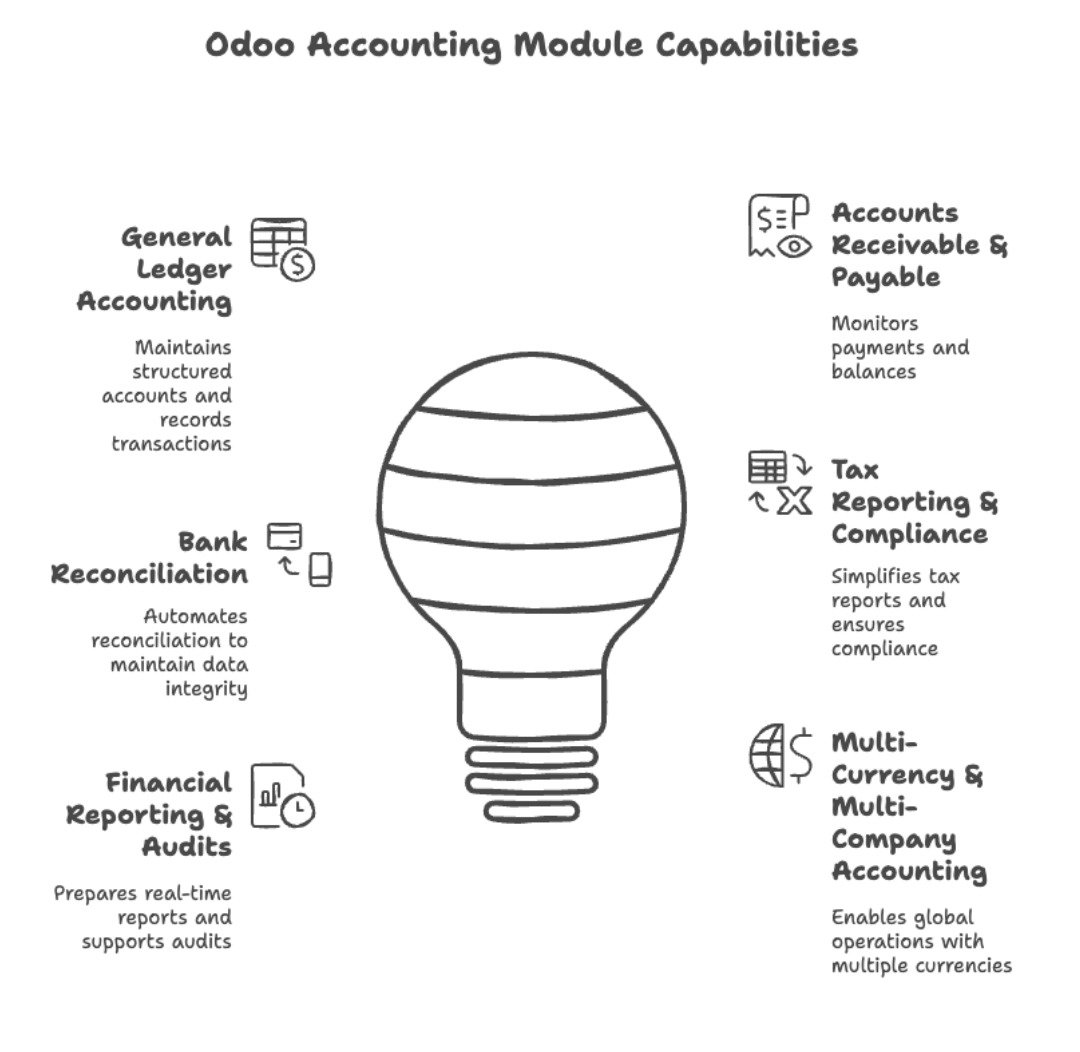
\includegraphics[width=0.8\linewidth]{diagram/odoo_accounting_module_capabilities.png}
\end{center}

\noindent\textbf{General Ledger Accounting}

\noindent Maintains a structured chart of accounts and records all financial transactions, which form the foundation for proper financial reporting.

\noindent\textbf{Accounts Receivable \& Accounts Payable}

\noindent Monitors payments received from customers and payments made to vendors, offering visibility and control over outstanding balances and obligations.

\noindent\textbf{Bank Reconciliation}

\noindent Automates reconciliation of bank statements with company records to identify discrepancies and maintain data integrity.

\noindent\textbf{Tax Reporting \& Compliance}

\noindent Simplifies the generation of tax reports and maintains compliance with local and foreign tax legislation, such as VAT, GST, and other statutory requirements.

\noindent\textbf{Financial Reporting \& Audits}

\noindent Prepares real-time financial reports such as balance sheets, income statements, and cash flow statements, and supports internal and external audit processes.

\noindent\textbf{Multi-Currency \& Multi-Company Accounting}

\noindent Enables global operations by permitting accounting in multiple currencies and processing consolidated or separate financials for several companies in a single Odoo instance.

\subsection{C4 Model - System Context Diagram (C1)}
\begin{center}
    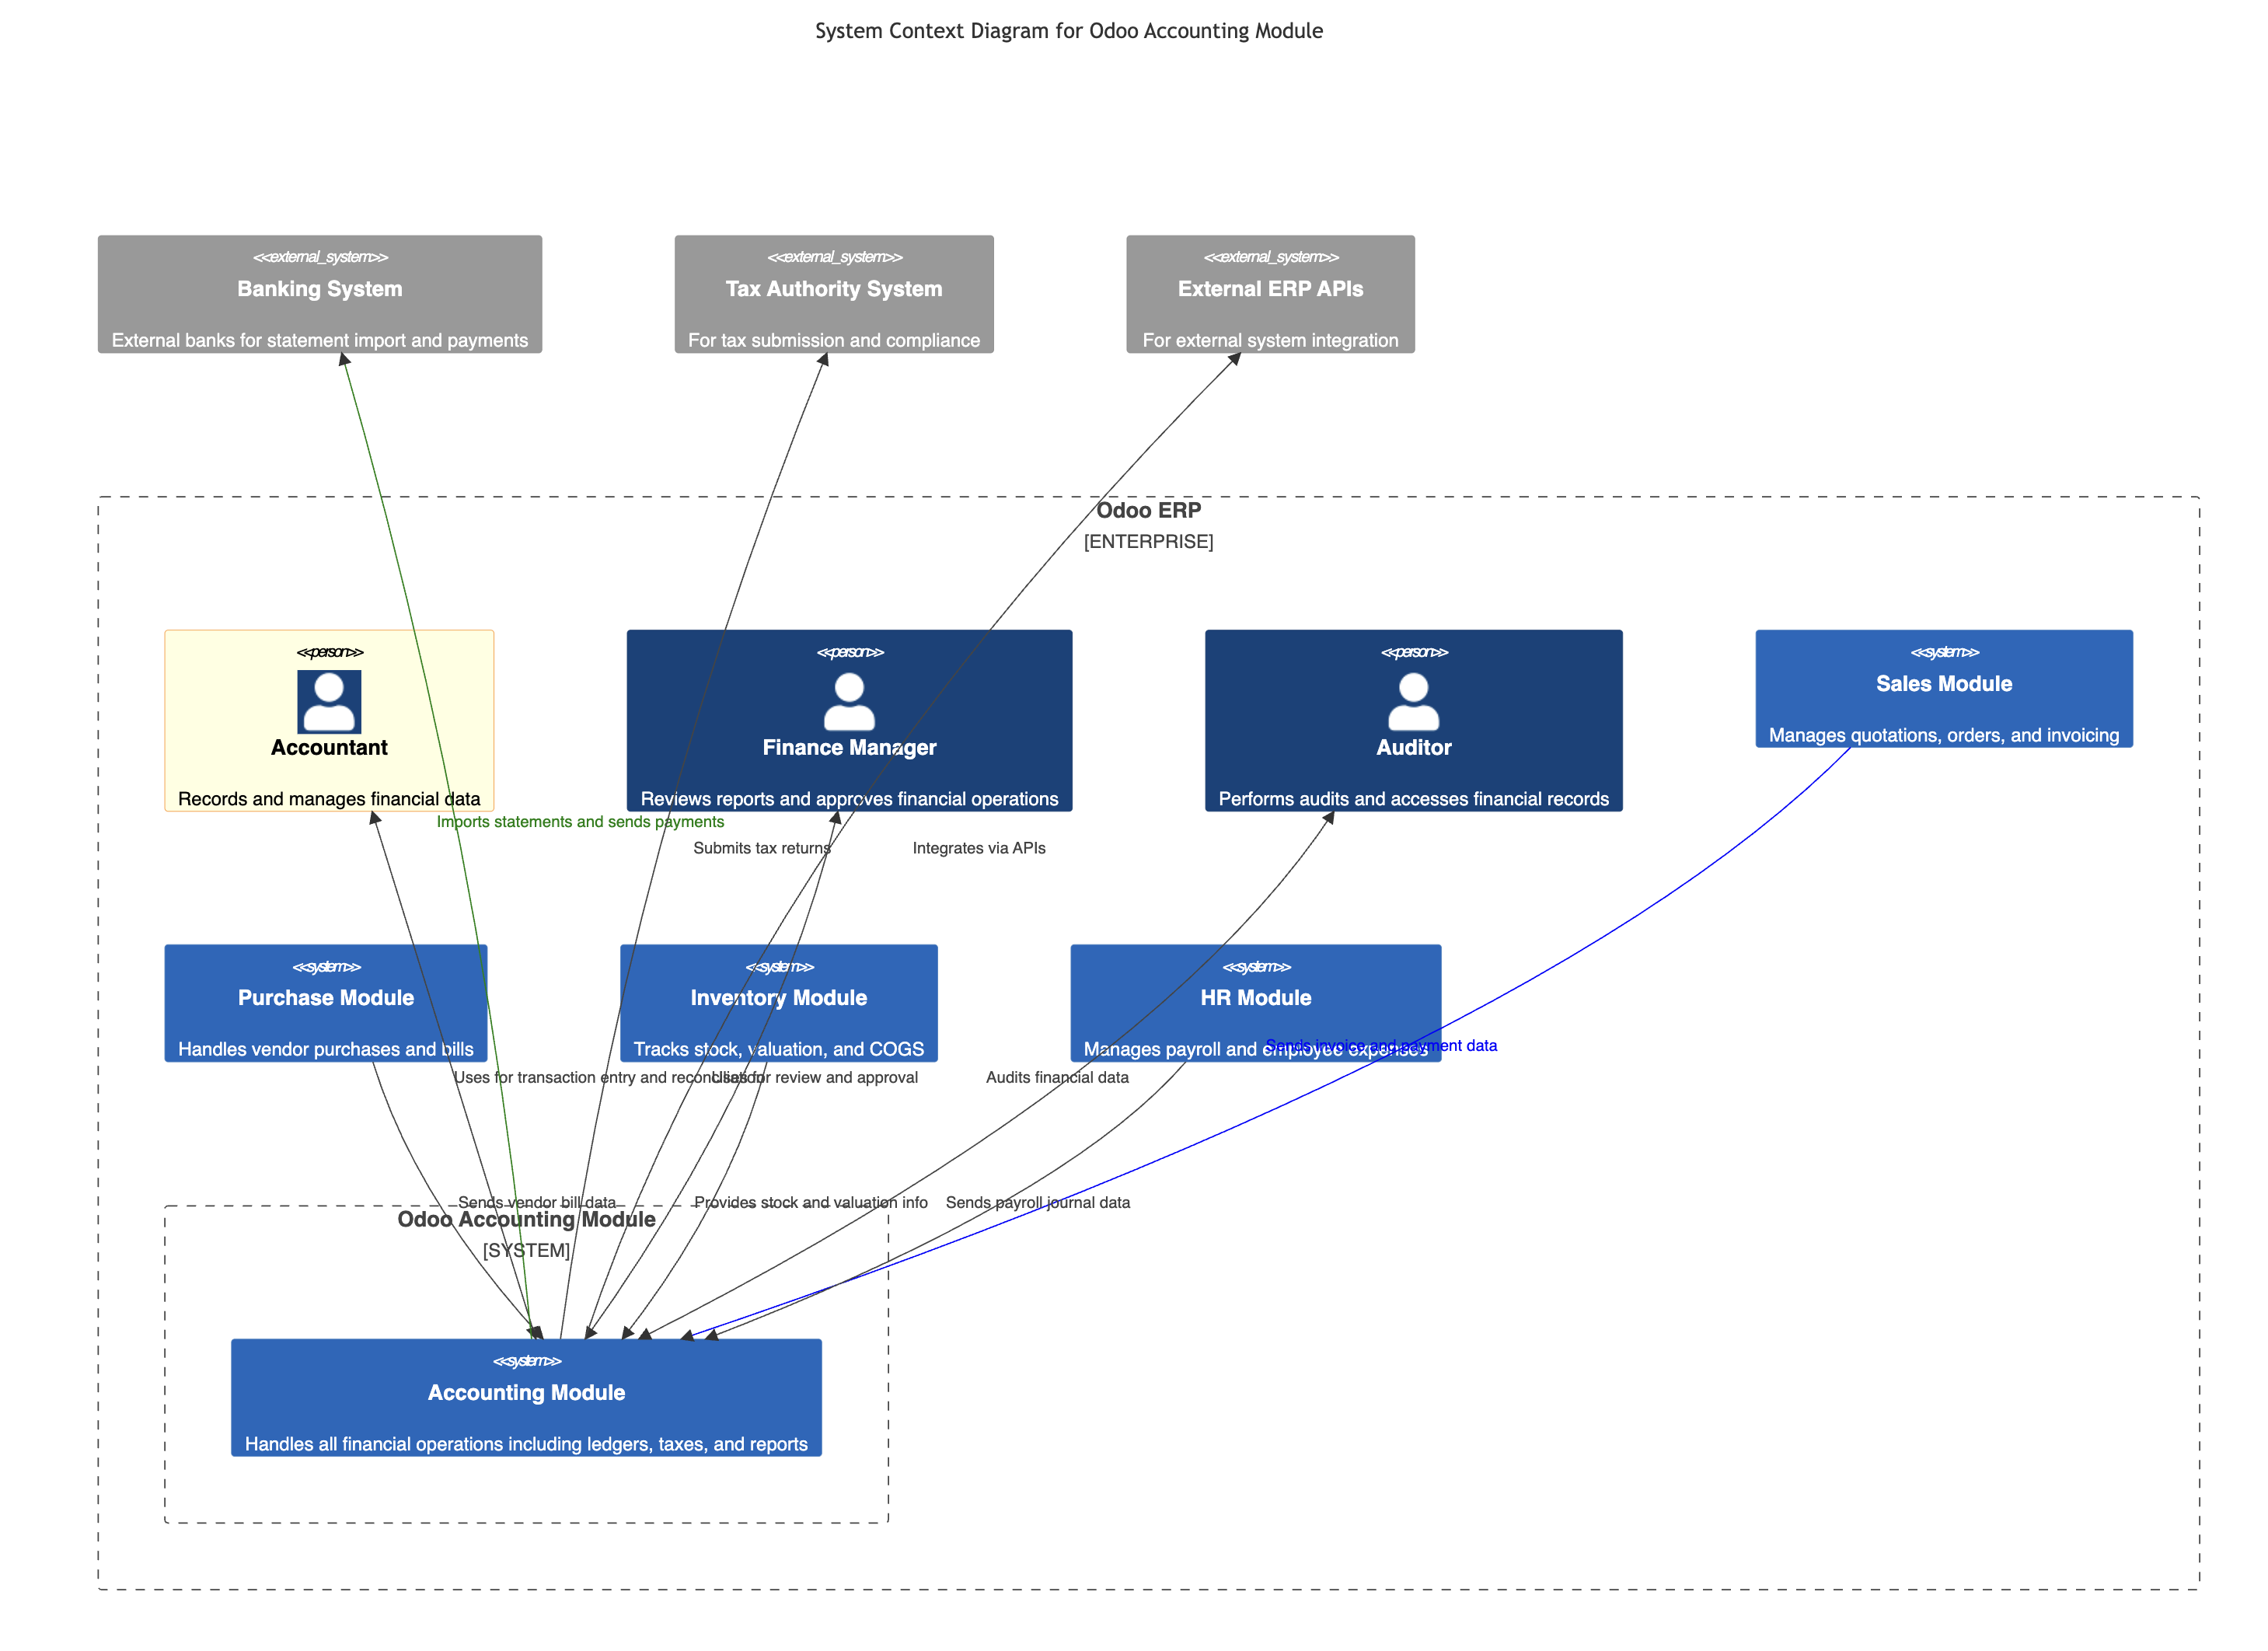
\includegraphics[width=0.8\linewidth]{diagram/C1.png}
\end{center}

\noindent The C1 diagram shows the big picture of how the Odoo Accounting Module fits into the Odoo system. It outlines the users, internal modules in communication, and external systems, but also focuses on how each talks to or depends upon the accounting module.
\bigskip
\noindent\textbf{Interactions:}

\noindent\textbf{Users:}
\begin{enumerate}[label=\roman*.]
    \item \textbf{Accountant:} Uses the accounting module to enter journal entries, process financial transactions, reconcile bank statements, and generate reports.
    \item \textbf{Finance Manager:} Generates financial reports, authorizes transactions, monitors cash flows, and verifies overall finance compliance via the module.
    \item \textbf{Auditor:} Puts accounting records into perspective to perform audits, ensures compliance checks, and submits regulatory ones.
\end{enumerate}

\noindent\textbf{Internal Odoo Modules:}
\begin{enumerate}[label=\roman*.]
    \item \textbf{Sales Module:} Sends customers' invoice and payment information to the accounting module for accounting revenues and monitoring receivables.
    \item \textbf{Purchase Module:} Puts vendor bill and purchase transaction records into the module to process accounts payable.
    \item \textbf{Inventory Module:} Provides stock value and COGS information to the financial ledgers for updating.
    \item \textbf{HR Module:} Updates payroll, employee expense reimbursements, and salary-related journal entries into the accounting system.
\end{enumerate}

\noindent\textbf{External Systems:}
\begin{enumerate}[label=\roman*.]
    \item \textbf{Banking System:} Exchanges information bi-directionally with the accounting module. Imports bank statements for reconciling. Exports payment instructions for vendor payments and salary payments.
    \item \textbf{Tax Authority System:} Accepts tax filings and compliance reports sent via the accounting module.
    \item \textbf{External ERP APIs:} Allows integration with third-party ERP systems for data exchange, e.g., invoices, payments, or financial summaries.
\end{enumerate}

\noindent\textbf{Dependencies:}
\begin{enumerate}[label=\roman*.]
    \item \textbf{Data from other Odoo modules:} Depends on the Sales, Purchase, Inventory, and HR modules to automatically receive transaction data, minimizing manual data entry and errors.
    \item \textbf{External banking integration:} Depends on connectivity to banking systems for statement imports and automatic payments.
    \item \textbf{Tax system access:} Depends on integration with government or regional tax authority systems for compliant reporting.
    \item \textbf{API integration:} Connects through APIs to connect with external ERPs, enhancing interoperability and facilitating real-time financial visibility across the platform.
    \item \textbf{User roles and access control:} Requires proper user role configurations to enable secure and compliant access for accountants, managers, and auditors.
\end{enumerate}

\noindent\textbf{Summary}

\noindent Interactions determine who uses the module and what systems send/receive data. Dependencies emphasize systems and sources of data required by the accounting module to accurately and efficiently operate. Combined, these linkages place the accounting module at the center of business operations, facilitating smooth financial management within and between departments and systems.

\newpage
\section{Finance \& Accounting Architecture Context}
\subsection{Module Architecture}
The Odoo Accounting module consists of several combined elements which, collectively, make a solid and combined finance administration solution. They are designed so that they support any number of accounting processes and they stay precise, compliant, and easy to use:

\begin{center}
    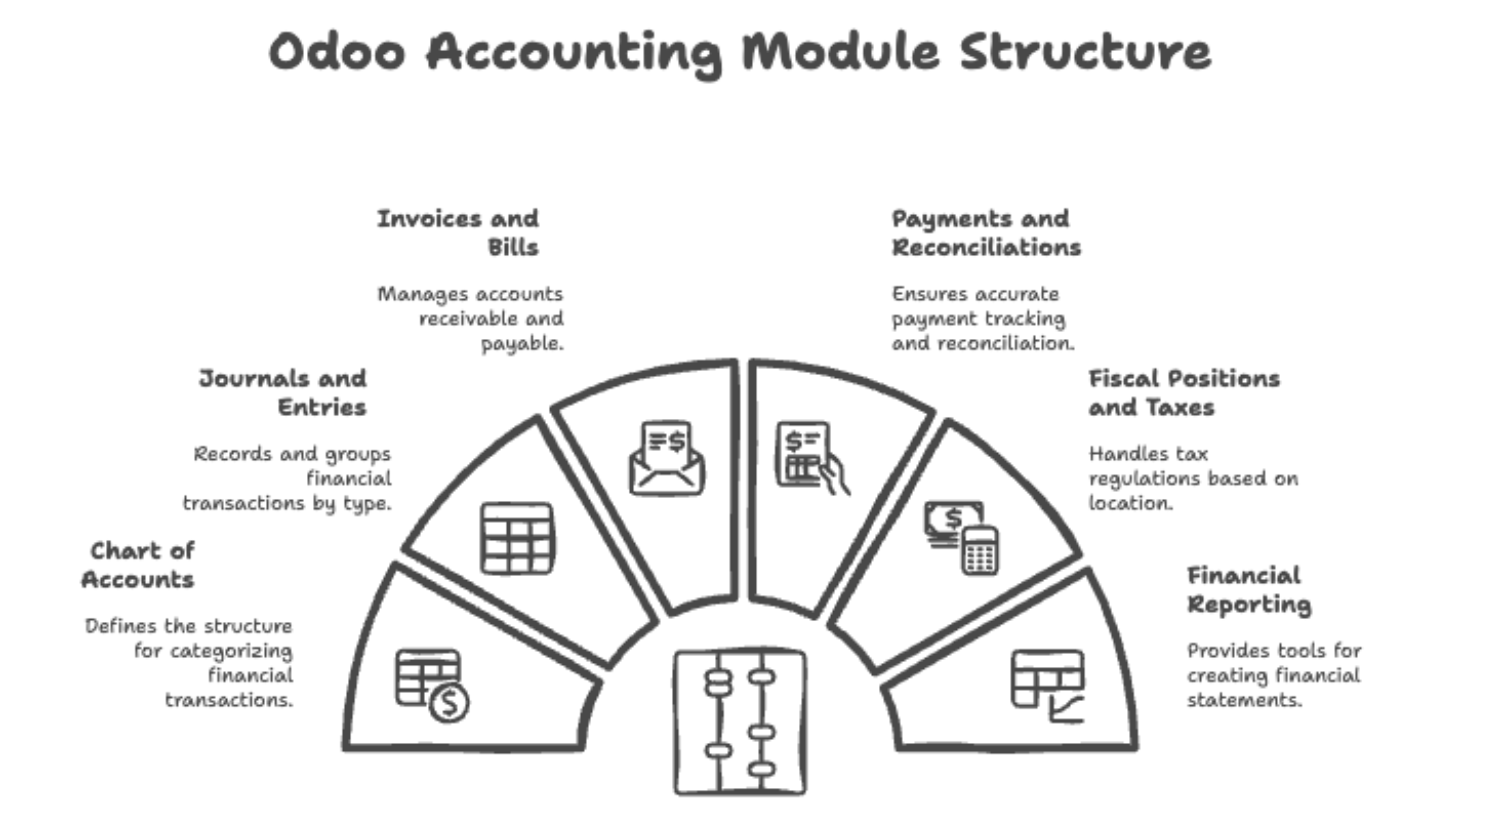
\includegraphics[width=0.8\linewidth]{diagram/odoo_accounting_module_structure.png}
\end{center}

\noindent\textbf{Chart of Accounts}

\noindent As the backbone of the accounting system, the Chart of Accounts defines the accounts that are used to categorize and post all financial transactions. It is a hierarchical and standardized structure that facilitates structured financial information across the organization.
\medskip

\noindent\textbf{Journals and Journal Entries}

\noindent Financial transactions are entered in journals, with one journal entry representing a definite business transaction (e.g., sale, purchase, payment). Different types of journals—such as sales, purchases, cash, or miscellaneous—help to group and trace transactions by their nature and source.
\medskip

\noindent\textbf{Invoices and Bills}

\noindent Invoices are issued to customers to request payment for goods or services, while bills are received from suppliers as account of amounts owed. The documents are crucial in managing accounts receivable and accounts payable to record both incoming and outgoing payments correctly.
\medskip

\noindent\textbf{Payments and Reconciliations}

\noindent This module manages capture of payments received from customers and payments made to suppliers. Reconciliation features embedded in the application allow users to reconcile payments with their corresponding invoices or bills for proper, up-to-date financial records and proper bank reconciliations without any errors.
\medskip

\noindent\textbf{Fiscal Positions and Tax Configuration}

\noindent Fiscal positions allow for dynamic handling of tax regulations based on customers' and vendors' location or status. This ensures that tax calculations are correct and in accordance with local and international tax legislation, especially in multi-jurisdictional settings.
\medskip

\noindent\textbf{Financial Reporting Tools}

\noindent Odoo Accounting has a robust set of reporting tools which enable the creation of financial statements such as balance sheet, profit \& loss, tax reports, audit-ready transaction histories, and analytical reports customized to specific requirements. The above-mentioned information helps in strategic decision-making and facilitates financial transparency.

\subsection{Key Features and Workflows}
The Odoo Accounting module offers a comprehensive suite of features and workflows to manage various financial processes. Here's an overview:

\begin{center}
    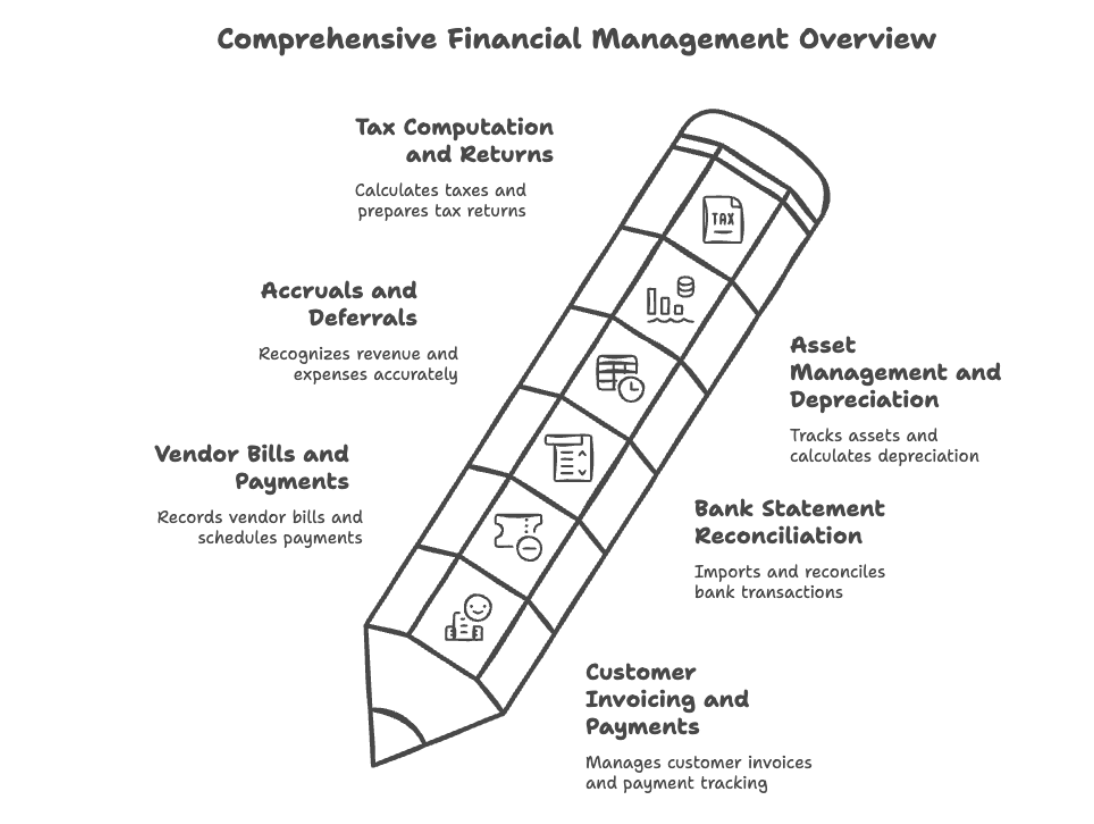
\includegraphics[width=0.8\linewidth]{diagram/comprehensive_financial_management.png}
\end{center}

\noindent\textbf{Customer invoicing and payments:} Create and manage customer invoices, track payments, and automate payment reminders.

\noindent\textbf{Vendor bills and payments:} Record and manage vendor bills, schedule payments, and track payment history.

\noindent\textbf{Bank statement reconciliation:} Import bank statements, match transactions, and reconcile bank accounts.

\noindent\textbf{Accruals and deferrals:} Recognize revenue and expenses in the correct accounting period, regardless of when cash changes hands.

\noindent\textbf{Asset management and depreciation:} Track fixed assets, calculate depreciation, and manage asset disposal.

\noindent\textbf{Tax computation and returns:} Calculate taxes on transactions, generate tax reports, and prepare tax returns.

\newpage
\noindent\textbf{Key Workflows:}

\medskip
\noindent\textbf{Sales-To-Cash:}

\noindent
\begin{minipage}{0.5\textwidth}
\begin{enumerate}
    \item Create a sales order.
    \item Confirm the sales order.
    \item Deliver the product/service.
    \item Create an invoice.
    \item Send the invoice to the customer.
    \item Receive payment from the customer.
    \item Reconcile the payment with the invoice.
\end{enumerate}
\end{minipage}%
\hfill
\begin{minipage}{0.45\textwidth}
    \centering
    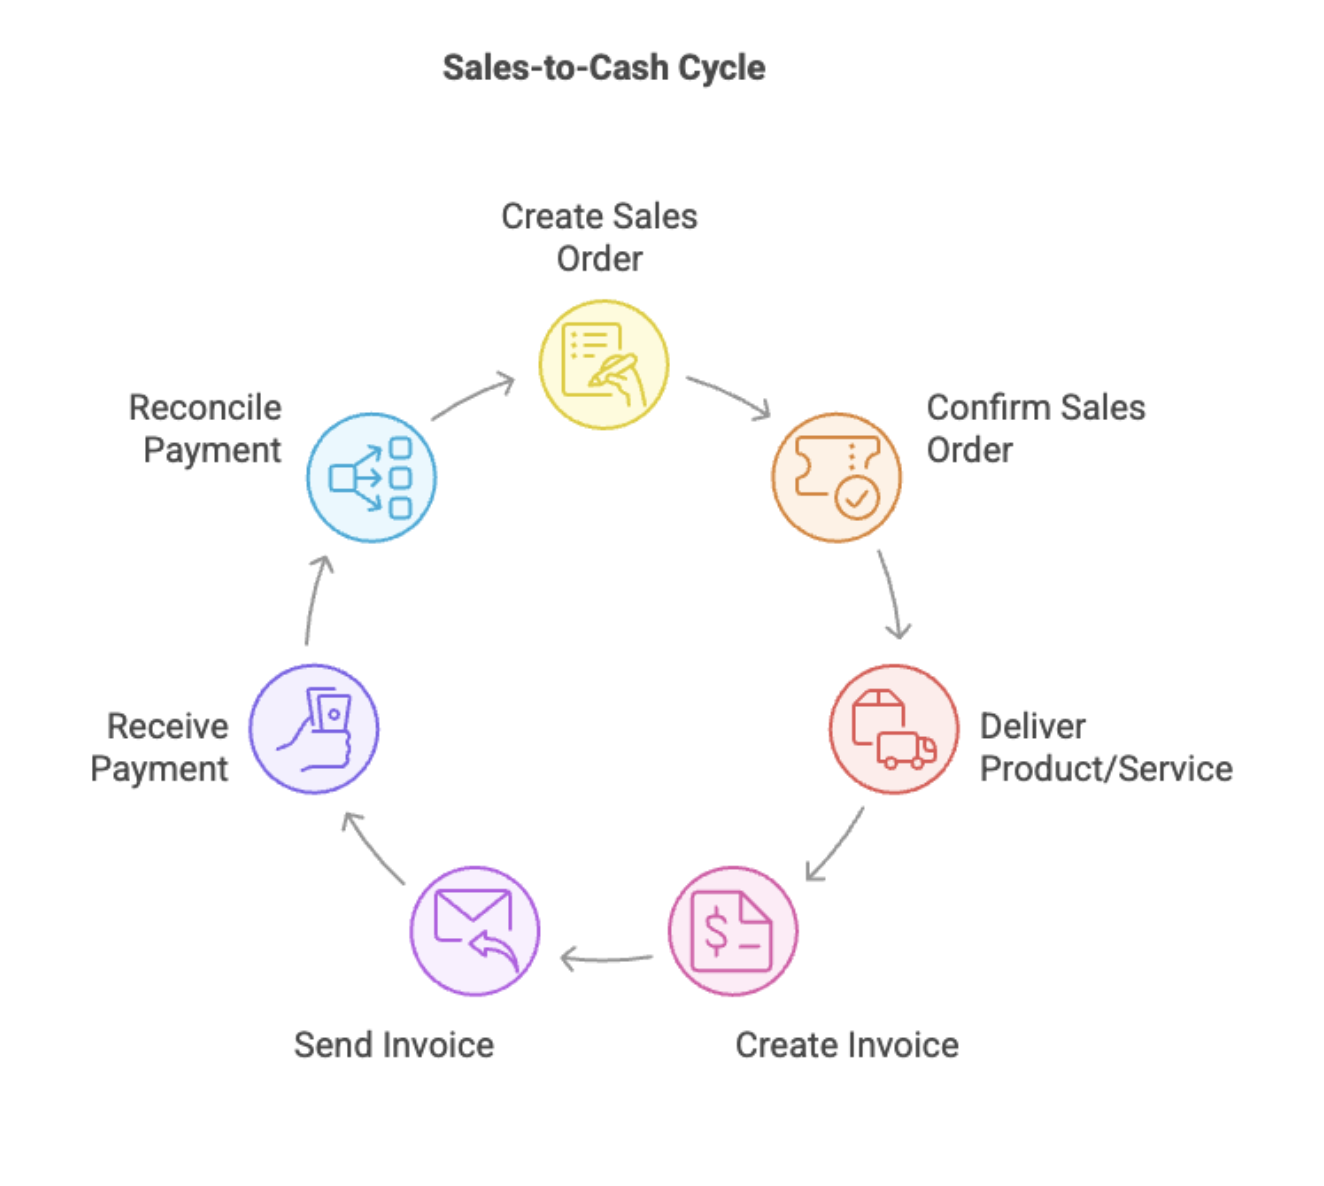
\includegraphics[width=\linewidth]{diagram/sales_to_cash_cycle.png}
\end{minipage}

\medskip
\noindent\textbf{Example:}
\begin{enumerate}
    \item \textbf{Create a Sales Order} \\
    Corporate customer, TechHive Ltd., contacts Big Business Cafe to order coffee and snacks for a seminar. \\
    Salesperson creates a Sales Order in Odoo:
    \begin{tabular}{l c c}
        \textbf{Product} & \textbf{Quantity} & \textbf{Price} \\
        Espresso & 100 cups & Rs 200 \\
        Croissants & 50 pieces & Rs 150 \\
        & \textbf{Total} & \textbf{Rs 350} \\
    \end{tabular}

    \item \textbf{Validate the Sales Order} \\
    Sales Order is validated in Odoo. This action keeps stock reserved and triggers delivery process.

    \item \textbf{Deliver the Product/Service} \\
    Staff delivers the 100 cups of coffee and 50 croissants to TechHive's seminar room on the day of the event. The Delivery Order status is marked as completed in Odoo.

    \item \textbf{Generate an Invoice} \\
    As soon as the delivery is confirmed, the system allows generating an invoice. An invoice for Rs 350 can be generated and is ready to send.

    \item \textbf{Send the Invoice to the Customer} \\
    The invoice is sent automatically from Odoo to TechHive's accounts department. A PDF invoice is automatically attached.

    \item \textbf{Get Payment from the Customer} \\
    After one week, TechHive Ltd., pays the invoice via bank transfer. The payment is recorded in Odoo as Customer Payments.

    \item \textbf{Reconcile the Payment with the Invoice} \\
    Once the bank statement is imported or synced, the payment is reconciled with the invoice. The invoice status is now Paid.
\end{enumerate}

\newpage
\noindent\textbf{Procure-to-Pay:}

\noindent
\begin{minipage}{0.5\textwidth}
\begin{enumerate}
    \item Create a purchase order.
    \item Confirm the purchase order.
    \item Receive the product/service.
    \item Receive a vendor bill.
    \item Approve the vendor bill.
    \item Pay the vendor bill.
    \item Reconcile the payment with the bill.
\end{enumerate}
\end{minipage}%
\hfill
\begin{minipage}{0.45\textwidth}
    \centering
    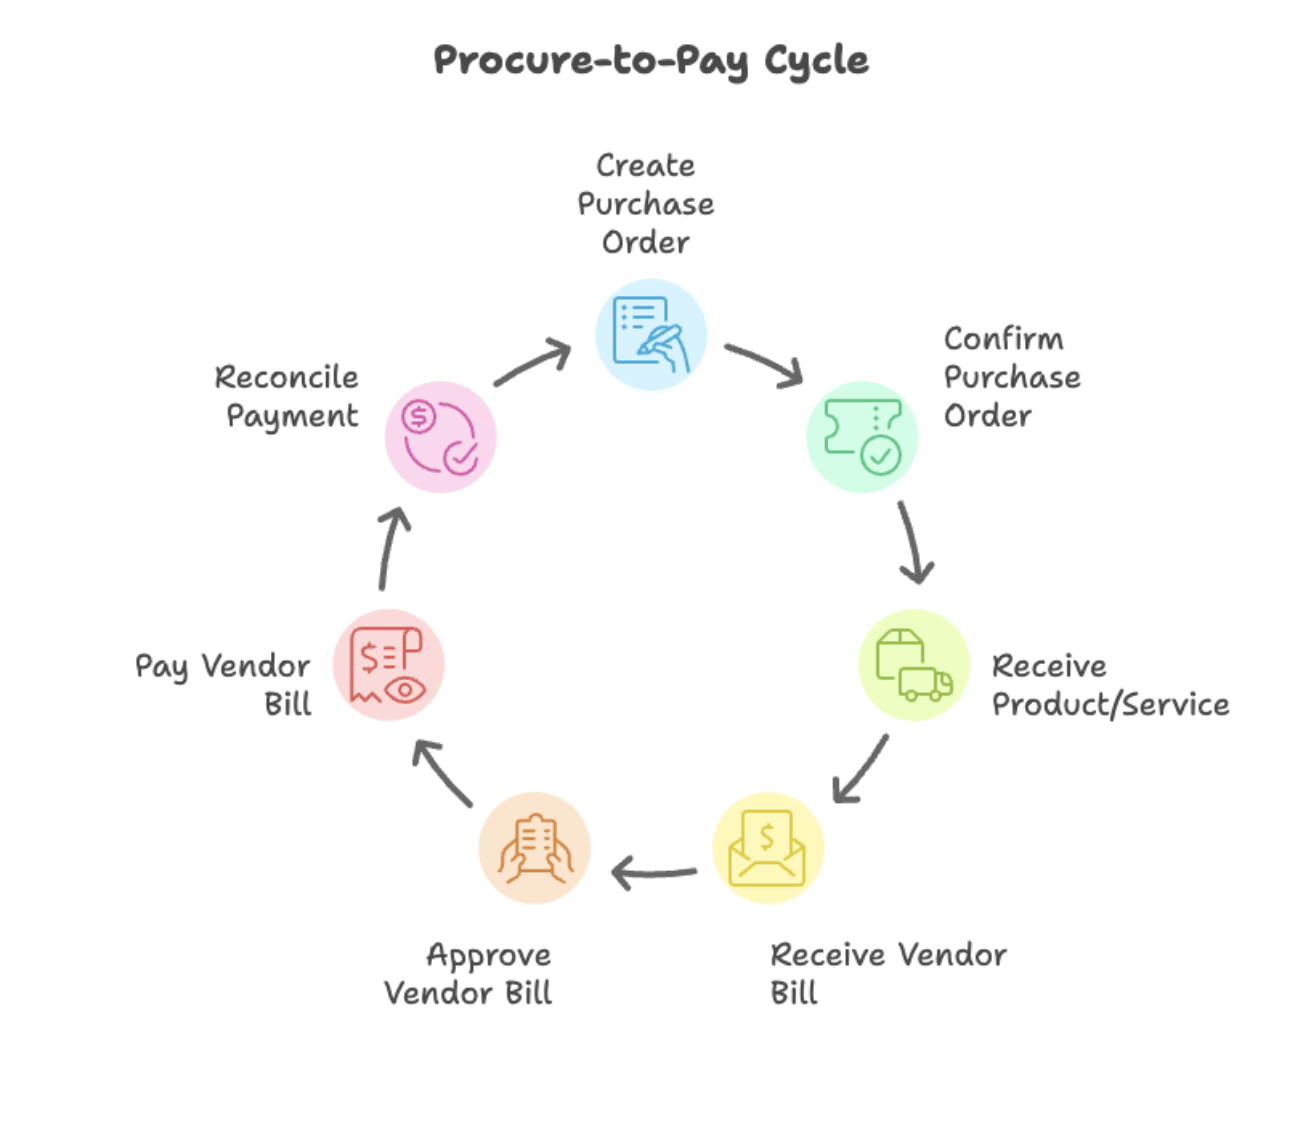
\includegraphics[width=\linewidth]{diagram/procure_to_pay_cycle.png}
\end{minipage}

\medskip
\noindent\textbf{Example:}
\begin{enumerate}
    \item \textbf{Create a Purchase Order} \\
    Big Business Cafe requires additional coffee beans and croissants. The purchasing manager creates a Purchase Order in Odoo to their supplier, FreshRoast Suppliers: \\
    \begin{tabular}{l c c}
        \textbf{Product} & \textbf{Quantity} & \textbf{Price} \\
        Premium Coffee Beans & 20 kg & Rs 300 \\
        Frozen Croissants & 200 pieces & Rs 400 \\
        & \textbf{Total} & \textbf{Rs 700} \\
    \end{tabular}

    \item \textbf{Confirm the Purchase Order} \\
    The PO is confirmed in Odoo. This notifies the supplier and starts expected delivery.

    \item \textbf{Receive the Product/Service} \\
    The supplier delivers the coffee beans and croissants to the cafe. The receiving team logs the delivery in Odoo by validating the Receipt.

    \item \textbf{Receive a Vendor Bill} \\
    FreshRoast Suppliers sends a Vendor Bill for Rs 700. The bill is posted in Odoo and matched with the original PO and receipt.

    \item \textbf{Approve the Vendor Bill} \\
    The bill is validated in Odoo by the finance manager for payment.

    \item \textbf{Pay the Vendor Bill} \\
    The payment (by bank transfer) is done and registered in Odoo in Vendor Payments.

    \item \textbf{Reconcile the Payment with the Bill} \\
    When the bank statement is synced or imported, the payment is reconciled with the vendor bill. The status of the bill is now Paid, and accounting is updated.
\end{enumerate}

\newpage
\noindent\textbf{Month-End Close:}

\begin{center}
    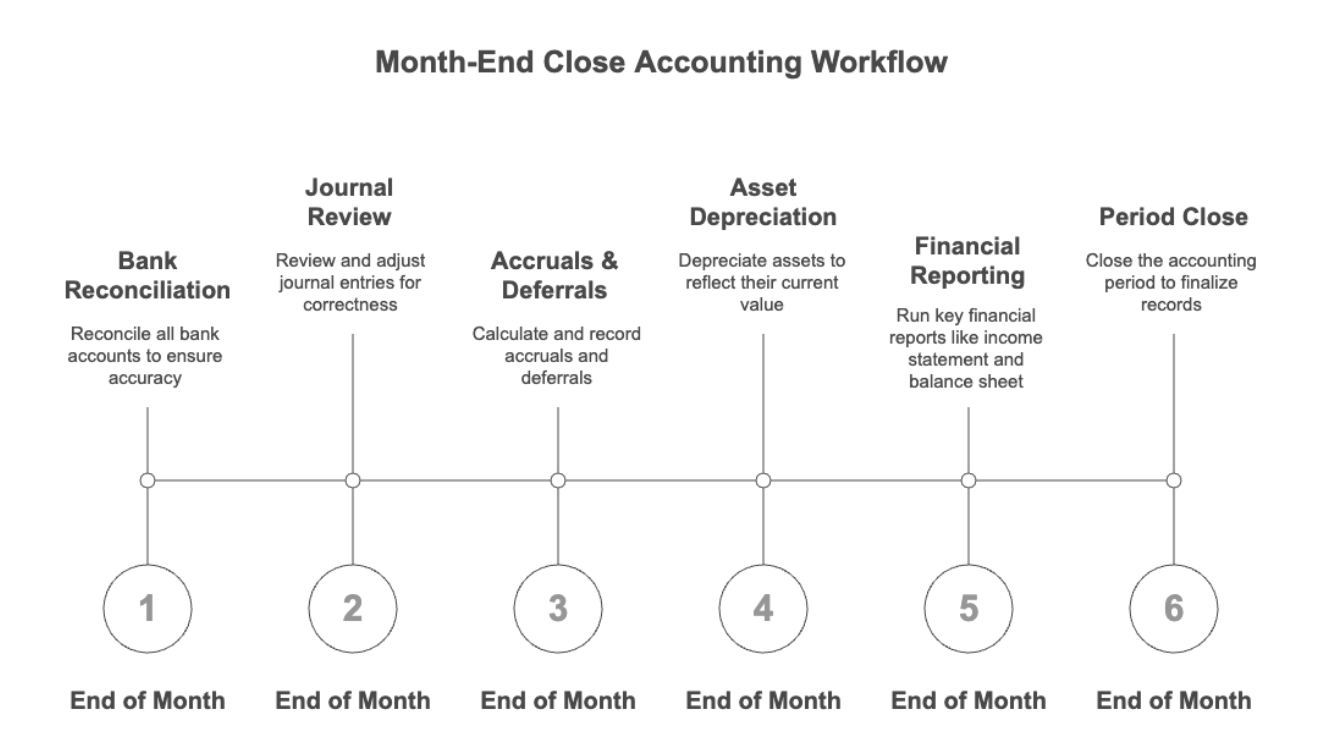
\includegraphics[width=0.8\linewidth]{diagram/month_end_close.png}
\end{center}

\begin{enumerate}
    \item Reconcile all bank accounts.
    \item Review and adjust journal entries.
    \item Calculate and record accruals and deferrals.
    \item Depreciate assets.
    \item Run financial reports (e.g., income statement, balance sheet).
    \item Close the accounting period.
\end{enumerate}

\medskip
\noindent\textbf{Example:}
\begin{enumerate}
    \item \textbf{Reconcile All Bank Accounts} \\
    Bank statements are downloaded by the accounting team using bank synchronization or CSV upload to Odoo. Customer payments (e.g., TechHive) and vendor payments (e.g., FreshRoast) are reconciled to invoices and bills. Transactions are reconciled to ensure no unmatched or outstanding entries exist.

    \item \textbf{Review and Adjust Journal Entries}
    
    The accountant verifies accuracy in the following entries:
    \begin{enumerate}
        \item Sales revenue
        \item Expense allocations (e.g., utilities, salaries, supplies)
        \item Manual rounding adjustments or corrections
    \end{enumerate}
    Adjusting entries are posted as necessary in Odoo to account for real economic activity.

    \item \textbf{Accrue and Record Accruals and Deferrals} \\
    \textbf{Accruals:} Rent owed this month but not yet received — a journal entry is recorded to accrue Rs 2,000. \\
    \textbf{Deferrals:} Prepaid catering service from a customer for the next month — revenue is deferred next period. \\
    These items are entered through Odoo's manual journal entry feature.

    \item \textbf{Depreciate Assets} \\
    The cafe has a coffee machine and some furniture that were indicated as fixed assets. With the Assets module in Odoo, depreciation each month is automatically calculated and posted as follows:
    \begin{enumerate}
        \item Coffee Machine - Rs 100 per month
        \item Furniture - Rs 50 per month
    \end{enumerate}

    \item \textbf{Print Financial Reports} \\
    The following are printed by the finance manager inside Odoo:
    \begin{enumerate}
        \item Income Statement (Profit \& Loss): revenue versus expenses
        \item Balance Sheet: verify assets, liabilities, and equity
        \item Cash Flow Statement: knowing liquidity
    \end{enumerate}

    \item \textbf{Close the Accounting Period} \\
    Upon review and approval, the accounting period is closed out in Odoo. This prevents further backdated entries and protects the period to be audited.
\end{enumerate}

\subsection{User Roles and Permissions}
Odoo has a fine-grained, customizable user roles and permissions system that ensures access to accounting functionality according to each user's responsibility. This structure provides protection for data, regulatory adherence, and effectiveness in the financial workflows.
\bigskip
\noindent\textbf{Default Roles}

\noindent Odoo is equipped with predefined default roles designed to meet common accounting tasks:
\bigskip

\noindent\textbf{Accountant:}

\noindent Accountants have wide access to the core functions of the accounting module. They can:
\begin{enumerate}
    \item Create and maintain customer invoices and vendor bills
    \item Record and confirm payments
    \item Post and amend journal entries
    \item Reconcile bank statements
    \item Generate financial and tax reports
\end{enumerate}

\noindent\textbf{Advisor:}

\noindent The Advisor role provides the highest level of access within the accounting module. In addition to all Accountant capabilities, Advisors can:
\begin{enumerate}
    \item Set up accounting parameters
    \item Maintain the chart of accounts and fiscal positions
    \item Perform sophisticated analysis and close accounting periods
    \item Manage financial compliance and audit processes
\end{enumerate}

\noindent\textbf{Role Mapping through Security Groups:}

\noindent Odoo uses security groups to define and control the access levels by role. Security groups dictate what data a user can view or edit, and what menus and actions are available to them. Examples:
\begin{enumerate}
    \item Accounting \& Finance / Accountant: Basic accounting access.
    \item Accounting \& Finance / Advisor: All access including configuration and sensitive actions
\end{enumerate}
Security groups are assigned to users through their role setup and can be changed accordingly.
\medskip

\noindent \textbf{Custom Roles:}

\noindent Custom roles can be created by companies to fit access for specific internal business processes or regulatory requirements. For instance:
\begin{enumerate}
    \item \textbf{Auditor} \\
    Read-only role that grants access to all relevant financial data but cannot be changed. Ideal for internal or external auditors to look at records and generate audit reports without fear of data modification.

    \item \textbf{Junior Accountant} \\
    A restricted role to perform core data entry activities such as posting invoices, bills, and performing simple reconciliations. Access rights can restrict visibility to confidential activities such as approving payments, modifying the chart of accounts, or period-end closings.
\end{enumerate}

\noindent\textbf{Creating a Custom Role in Steps}
\begin{enumerate}
    \item \textbf{Copy an Existing Role} \\
    Begin from an existing role (e.g., Accountant) so that there is a foundation to start from a set of common permissions.

    \item \textbf{Modify Associated Security Groups} \\
    Set up the security groups to fine-tune the degree of access. You may turn on or turn off access to specific models, views, menus, and reports.

    \item \textbf{Assign the Role to Users} \\
    Once you've established the custom role, assign the role to the designated users via their user profile.
\end{enumerate}

\noindent This roles-and-permissions framework enables companies to enforce proper segregation of duties and responsibility upon accounting procedures, but remain flexible enough to compensate for shifting organization needs.

\subsection{C4 Model - Container Diagram (C2)}
\begin{center}
    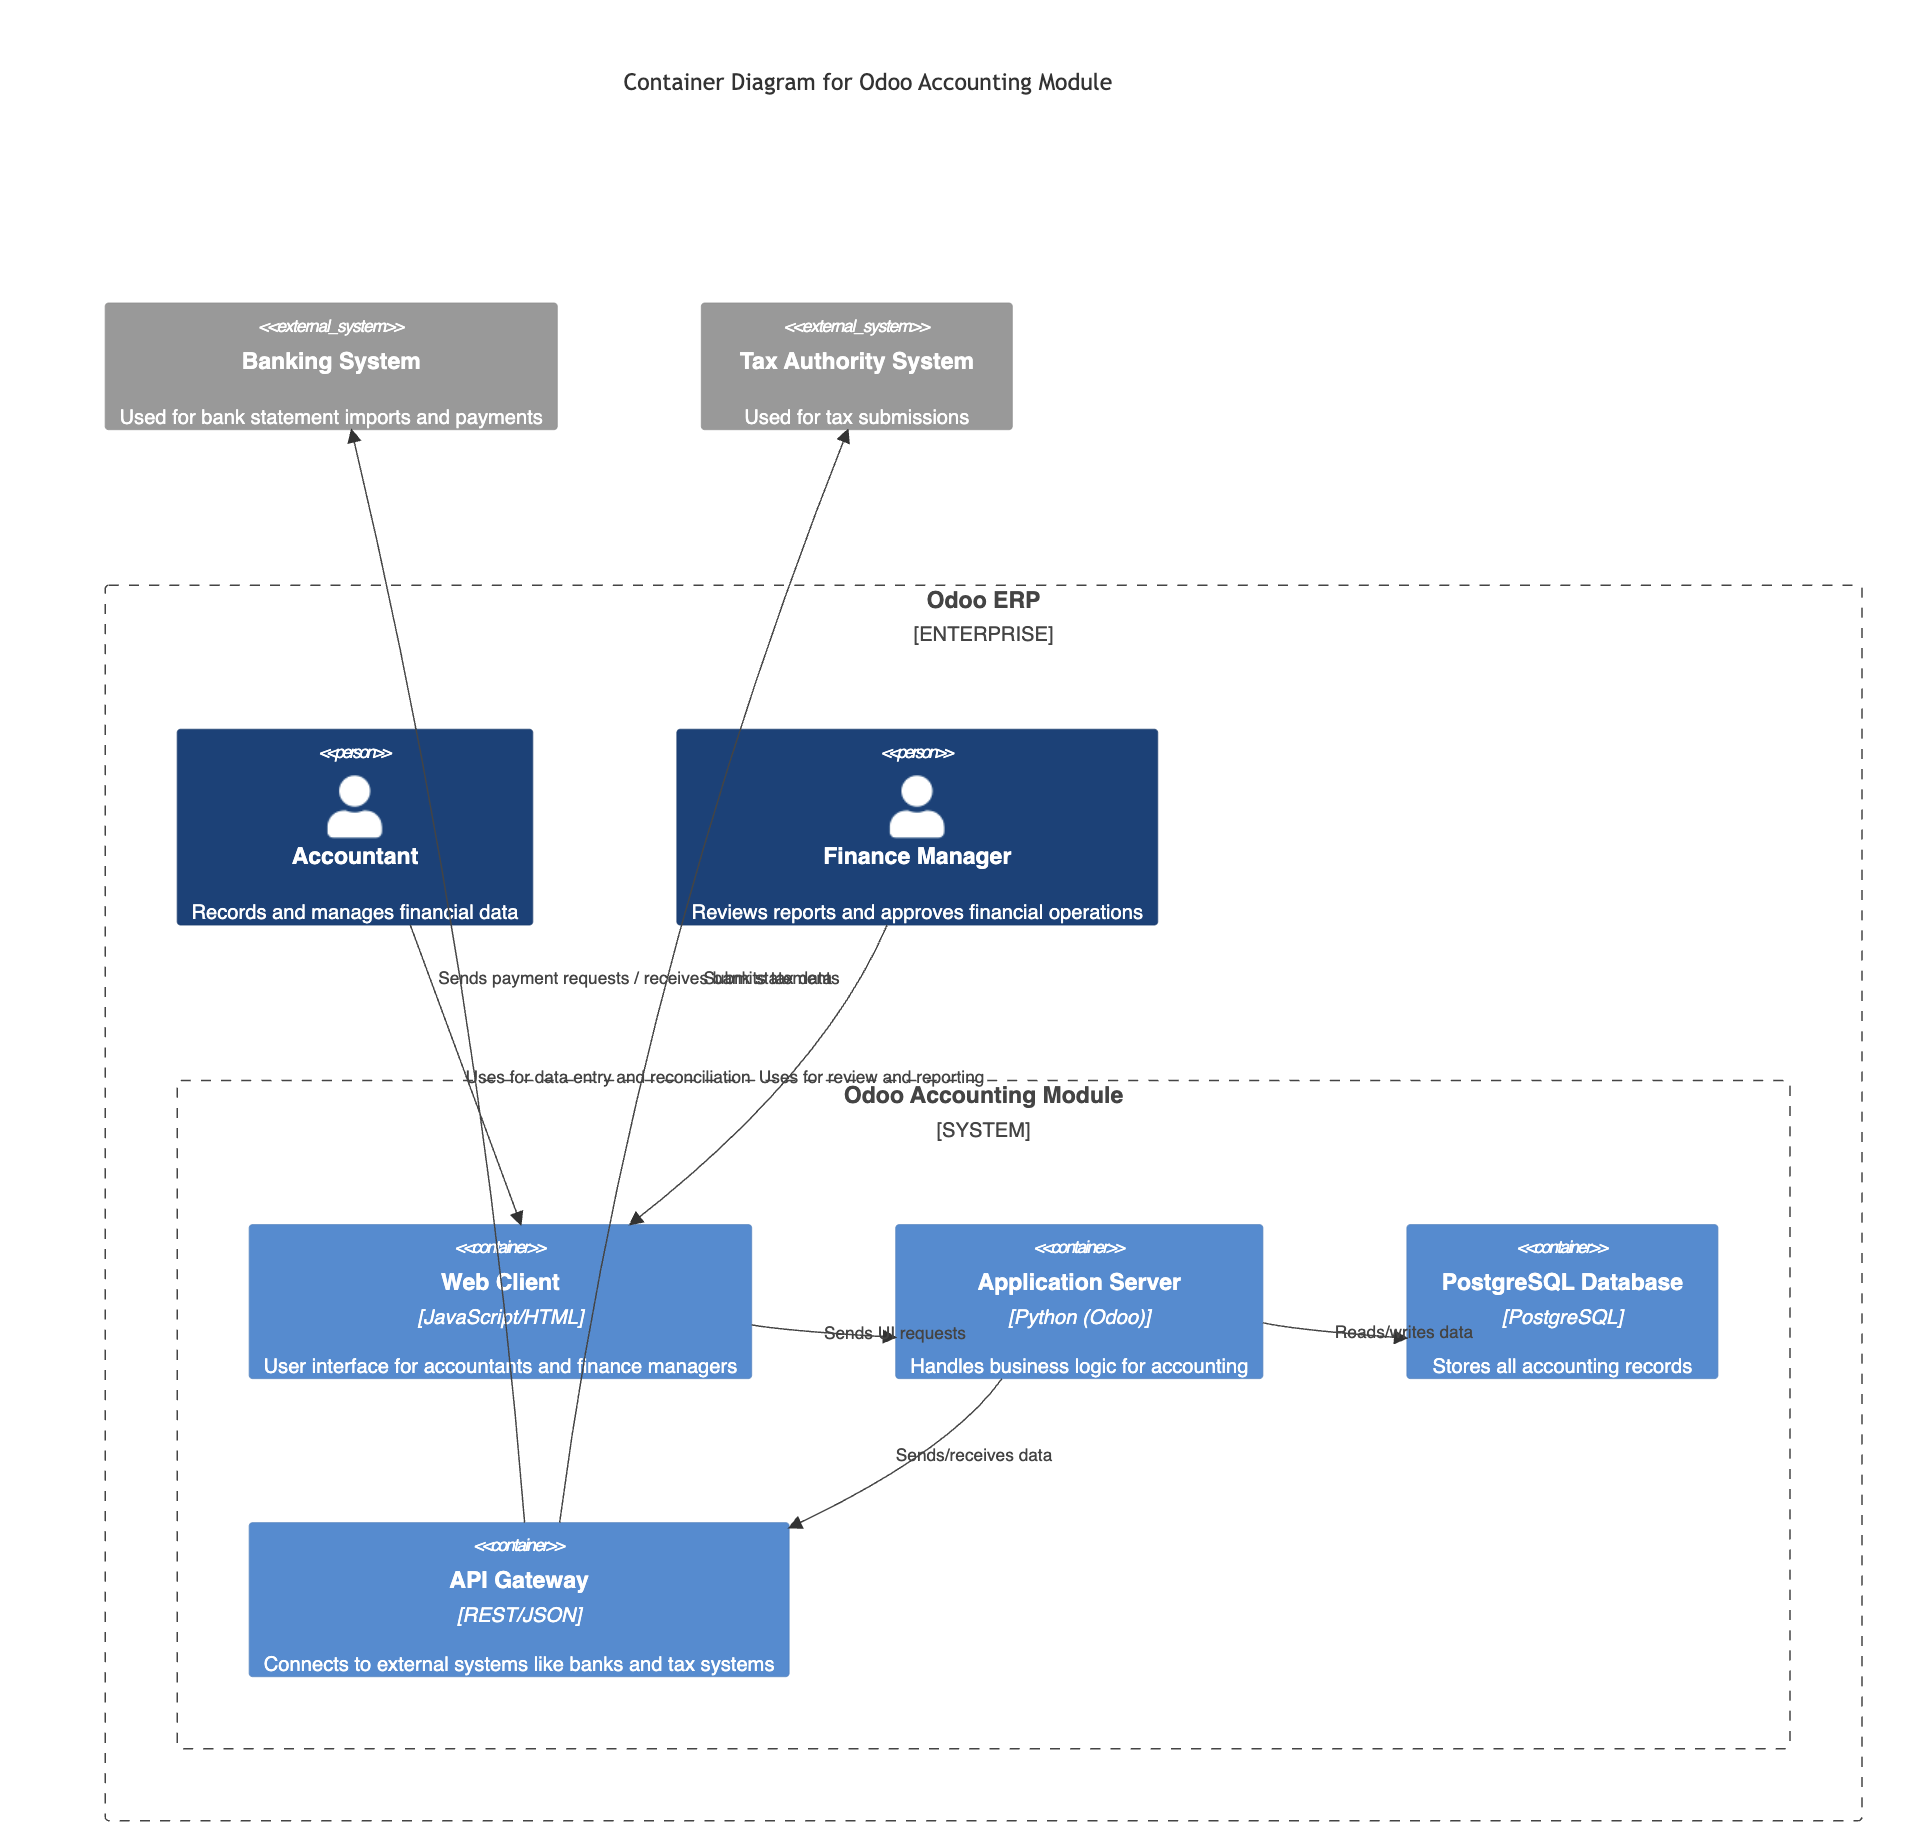
\includegraphics[width=0.8\linewidth]{diagram/C2.png}
\end{center}

\noindent The C2 diagram highlights Odoo Accounting module technical architecture by depicting its major containers and how they interact. They include the Odoo server, the PostgreSQL database, and the Web client. Together, they form the system runtime and data-processing environment core.
\medskip

\noindent In the middle lies the Odoo Server, built using Python for business logic and XML for views and configuration. The server addresses all critical accounting tasks, including invoice management, journal entry, reconciliation of accounts, and reporting. Workflow logic is managed by the server, and communication from the database to the user interface is planned.
\medskip

\noindent The PostgreSQL database serves as the persistent storage for all the accounting information customer invoices, vendor bills, journal entries, tax information, and reporting information. All of the transactions initiated on the server are stored and retrieved within this robust relational database system, ensuring data integrity and transaction validity.
\medskip

\noindent The Web client, developed using JavaScript, provides the front-end interface through which users like finance managers and accountants interact with the system. These include the generation of invoices, looking at financial dashboards, bank statement reconciliation, and the generation of financial reports. The web client communicates in real-time with the Odoo server via RPC and REST calls to fetch or send data.
\bigskip

\noindent\textbf{Data Flows}

\noindent\textbf{Invoice Creation → Journal Entry Generation:}
When a user posts a customer invoice through the web client, the data is sent to the Odoo server, and journal entries for the invoice are created automatically. The entries are committed to the PostgreSQL database.

\noindent\textbf{Real-Time Posting and Report Generation:}
While transactions are being posted, financial records are updated in real-time by the system. Users can instantly view updated balance sheets, profit \& loss statements, and tax summaries from the web interface due to the smooth data sync between the Odoo server and PostgreSQL.
\medskip

\noindent This kind of architecture delivers a responsive, scalable, and highly integrated accounting experience within the Odoo ERP environment, enabling accurate and real-time financial management.

\newpage
\section{Data Structure and Relationships}
\subsection{Key Data Models}
Odoo's Accounting module is developed around several major models that complement one another to form a complete and accurate financial system. Below is an improved analysis of the most important models, their business impact, primary fields, and relation.

\begin{enumerate}
    \item \textbf{account.move (Journal Entries)}
    
    \textbf{Business Significance:}

    Is a journal entry, the most basic double-entry bookkeeping unit. It records economic transactions between accounts.
    \medskip

    \textbf{Key Fields:}

    name (Char): Reference to journal entry (auto-generated sequence). 

    date (Date): Date of transaction.

    journal\_id (Many2one): Journal it belongs to (e.g., Sales, Purchase). 

    company\_id (Many2one): Company owning the entry. 

    state (Selection): Status (e.g., Draft, Posted).

    line\_ids (One2many): Journal lines belonging to this entry.

    amount\_total (Monetary): Total value of the transaction.
    \medskip

    \textbf{Relationships:}

    One-to-many with account.move.line

    Many-to-one with account.journal, res.company

    \item \textbf{account.move.line (Journal Items)}
    
    \textbf{Business Significance:}

    A line is a specific debit or credit in a journal entry. It defines the amount, account, and optionally, the related partner. 
    \medskip

    \textbf{Key Fields:}

    move\_id (Many2one): Parent journal entry. 

    account\_id (Many2one): Ledger account involved. 

    partner\_id (Many2one): Close customer/vendor.

    name (Char): Description of entry. 

    debit, credit (Monetary): Amounts. 

    amount\_currency (Monetary), currency\_id: Currency details. 

    tax\_ids (Many2many): Taxes applied.
    \medskip

    \textbf{Relationships:}

    Many-to-one with account.move, account.account, res.partner

    Many-to-many with account.tax

    \item \textbf{account.account (Chart of Accounts)}
    
    \textbf{Business Significance:}

    Creates individual accounts in the chart of accounts (COA) utilized to categorize transactions.
    
    \textbf{Key Fields:}

    code (Char): Alphanumeric account code.

    name (Char): Description of account.

    user\_type\_id (Many2one): Account type (income, expense, etc.).

    reconcile (Boolean): Whether reconcilable or not.

    company\_id (Many2one): The company it belongs to.
    \medskip

    \textbf{Relationships:}

    One-to-many with account.move.line

    Many-to-one with account.account.type, res.company 

    \item \textbf{account.payment (Payments)}
    
    \textbf{Business Significance:}

    Captures incoming/outgoing money flow for customer receipts and vendor payments.
    \medskip

    \textbf{Key Fields:}

    date (Date): Date of the payment.

    payment\_type (Selection): In or out.

    partner\_type (Selection): Customer or vendor.

    partner\_id (Many2one): Concerned party.

    amount (Monetary): Amount paid.

    currency\_id (Many2one): Used currency.

    journal\_id (Many2one): Origin journal.

    payment\_method\_id (Many2one): Means (e.g., check, wire).

    move\_id (Many2one): Related journal entry.
    \medskip

    \textbf{Relationships:}

    Many-to-one with res.partner, account.journal, account.payment.method, account.move

    \item \textbf{account.tax and account.fiscal.position}
    
    \textbf{account.tax}
    
    \textbf{Business Significance:}

    Specifies tax rules and rates for sales and purchases.
    \medskip

    \textbf{Key Fields:}

    name (Char): Tax name (e.g., VAT 13\%).

    amount (Float): Rate.

    amount\_type (Selection): Fixed, percentage, or division.

    type\_tax\_use (Selection): Sale, purchase, or both.

    account\_id (Many2one): Linked account for tax posting.
    \medskip

    \textbf{Relationships:}

    One-to-many with account.move.line
    \medskip

    \textbf{account.fiscal.position}
    
    \textbf{Business Significance:}

    Applies tax mappings for specific partner location or type. 
    \medskip

    \textbf{Key Fields:}

    name (Char): Position name (e.g., Export). 

    company\_id (Many2one): Related company.

    tax\_ids (One2many): Tax replacement rules.
    \medskip

    \textbf{Relationships:}

    Many-to-one with res.company, res.partner

    One-to-many with account.fiscal.position.tax

    \item \textbf{res.partner (Partners)}
    
    \textbf{Business Significance:}

    Stores contact data for all third parties—customers, vendors, etc.
    \medskip

    \textbf{Key Fields:}

    name, is\_company, street, city, country\_id

    vat: VAT number

    customer\_rank, supplier\_rank 

    property\_account\_receivable\_id: Default AR account 

    property\_account\_payable\_id: Default AP account 

    property\_payment\_term\_id, property\_supplier\_payment\_term\_id 

    fiscal\_position\_id: Default tax rule mapping 
    \medskip
    
    \textbf{Relationships:}

    One-to-many with account.move.line, account.payment

    Many-to-one with account.fiscal.position
\end{enumerate}

\begin{center}
    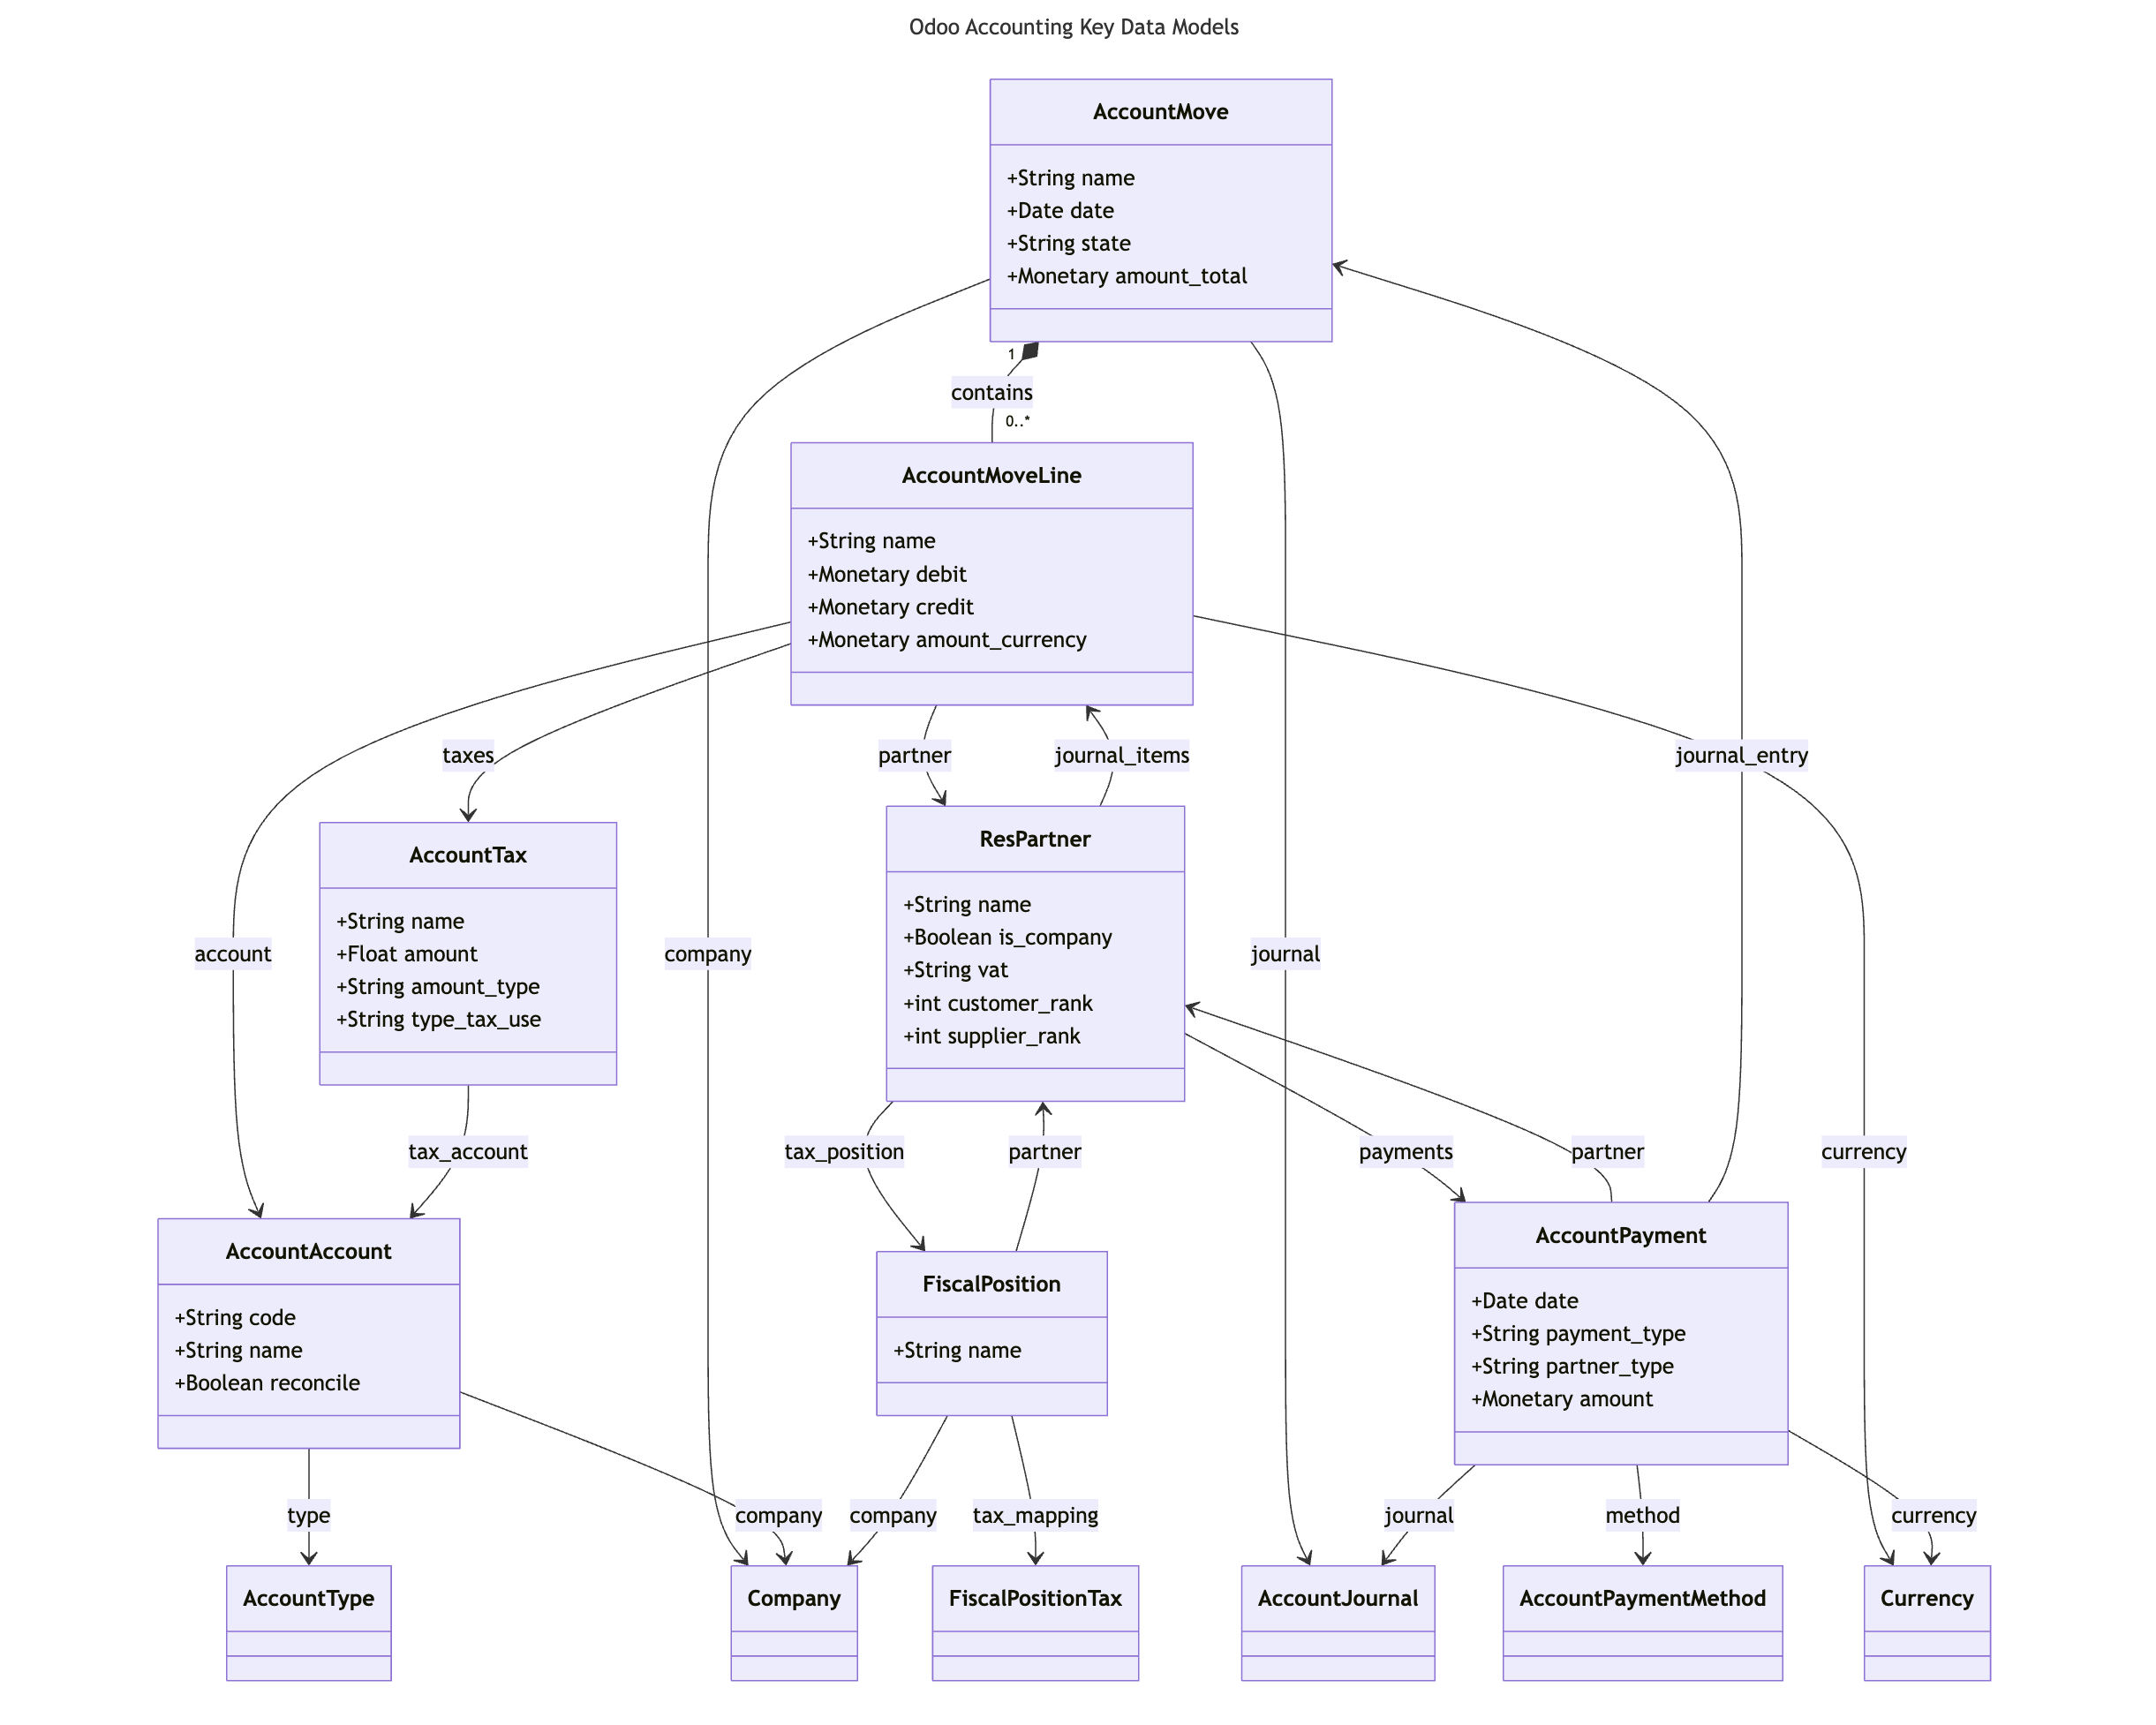
\includegraphics[width=0.8\linewidth]{diagram/odoo_accouting_key_data_models.png}
\end{center}

\subsection{Database Schema Overview}
This chapter explains the top database tables in Odoo's Accounting module and the foreign key relationships and constraints that ensure data integrity across the system.
\medskip

\noindent\textbf{Core Tables}
\medskip

\begin{tabular}{|l|p{10cm}|}
    \hline
    \textbf{Table} & \textbf{Description} \\
    \hline
    \texttt{account\_move} & Contains journal entries, the basic unit of double-entry accounting. \\
    \hline
    \texttt{account\_move\_line} & Contains individual debit/credit lines of a journal entry. \\
    \hline
    \texttt{account\_account} & Holds the Chart of Accounts — ledger accounts used for classifying transactions. \\
    \hline
    \texttt{account\_journal} & Stores definitions of journals such as Sales Journal, Purchase Journal, etc. \\
    \hline
    \texttt{account\_payment} & Stores payment postings such as customer receipts and vendor payments. \\
    \hline
    \texttt{account\_tax} & Declares tax regulations (e.g., VAT, service tax) for financial postings. \\
    \hline
    \texttt{account\_fiscal\_position} & Maps fiscal rules for partners by location or type of business. \\
    \hline
    \texttt{res\_partner} & Stores customer, vendor, and other third-party information. \\
    \hline
    \texttt{res\_company} & Stores company data, allowing multi-company setups. \\
    \hline
    \texttt{account\_account\_type} & Categorizes accounts into types such as Income, Expenses, Payable, etc. \\
    \hline
\end{tabular}

\newpage
\subsection{Data Flow Diagrams}
\noindent\textbf{Invoice}

\begin{minipage}{0.45\textwidth}
    \noindent\textbf{Purpose:} Shows how an invoice is created, 
    validated, paid, and optionally cancelled.
    \medskip

    \noindent\textbf{Steps:}
\begin{enumerate}
    \item Create Invoice Draft (account.move): An 
    invoice draft is made.
    \item Add Invoice Lines (account.move.line): Line items like products or services are added.
    \item Validate Invoice: The invoice is posted, 
    which makes accounting entries.
    \item Register Payment (account.payment): A 
    payment is recorded for the invoice.
    \item Update Invoice Record: The invoice is set 
    as paid.
    \item Reconcile Payment (account.partial.reconcile): Debits and credits are matched.
    \item Cancel Invoice (optional): Invoice is 
cancelled, reverting changes.
\end{enumerate}
\end{minipage}%
\hfill
\begin{minipage}{0.4\textwidth}
    \centering
    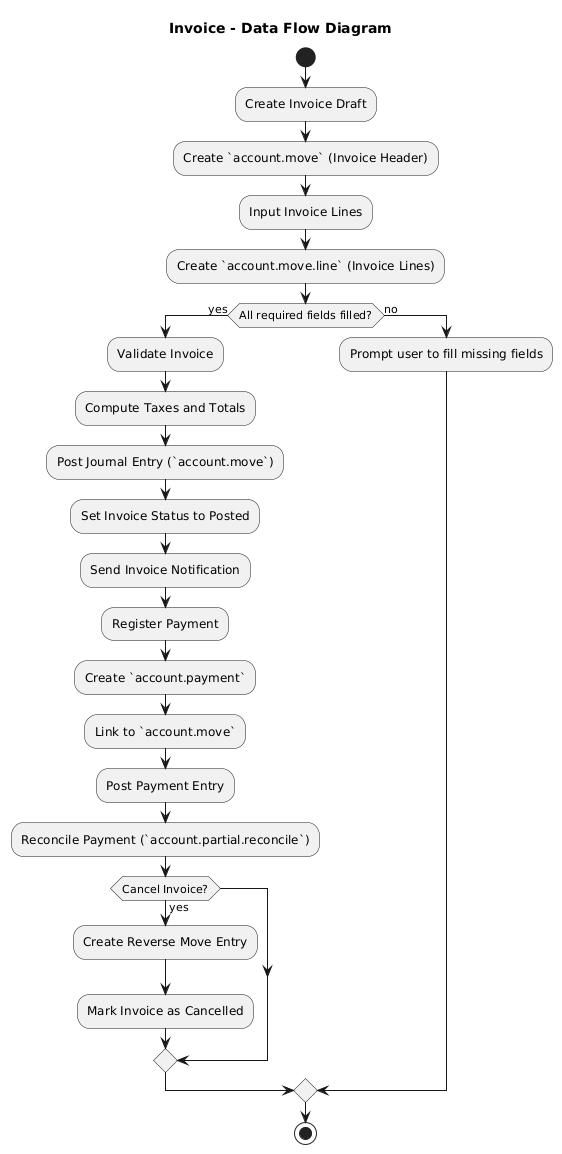
\includegraphics[width=\linewidth]{diagram/invoice-DFD.png}
\end{minipage}

\newpage
\noindent\textbf{Payment}
\medskip

\begin{minipage}{0.45\textwidth}
    \noindent\textbf{Purpose:} Shows payments 
    posted and processed to the 
    general ledger.
    \medskip
    
    \noindent\textbf{Steps:}
\begin{enumerate}
    \item Create Payment (account.payment): Payment, 
    either received or paid, is 
    posted.
    \item Specify Payment Details: 
    Currency, partner, and method 
    are defined.
    \item Post Payment: Payment is 
    checked.
    \item Generate Journal Entry 
    (account.move): Accounting 
    records for transaction are 
    generated.
    \item Generate Lines 
    (account.move.line): Debit and 
    credit lines are posted.
    \item Link to Invoice (account.partial.reconcile): Reconciles payment to invoice.
\end{enumerate}
\end{minipage}%
\hfill
\begin{minipage}{0.45\textwidth}
    \centering
    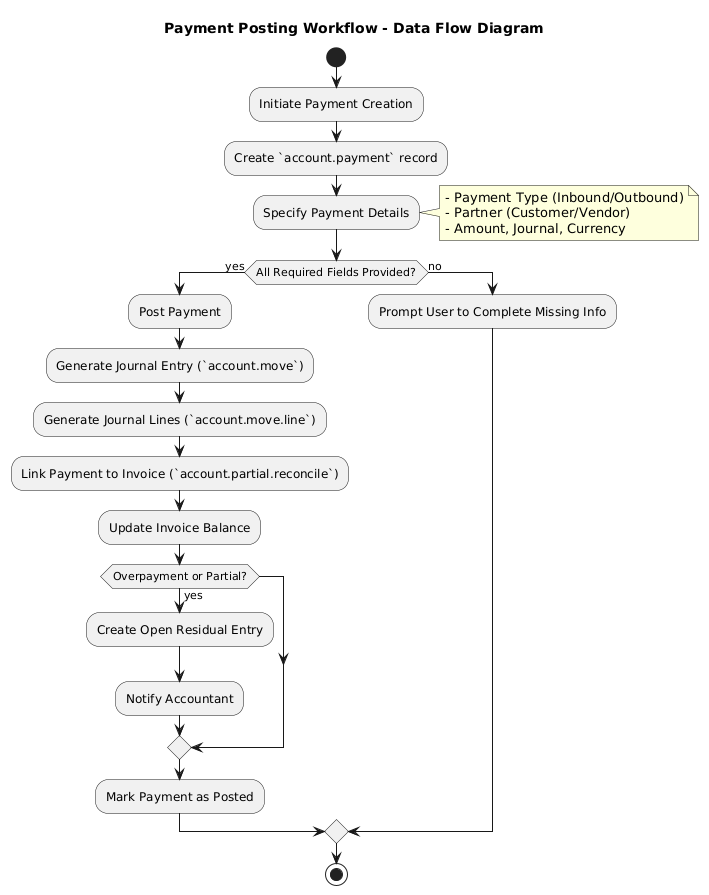
\includegraphics[width=\linewidth]{diagram/payment-DFD.png}
\end{minipage}

\newpage
\noindent\textbf{Bank Reconciliation}
\medskip

\begin{center}
    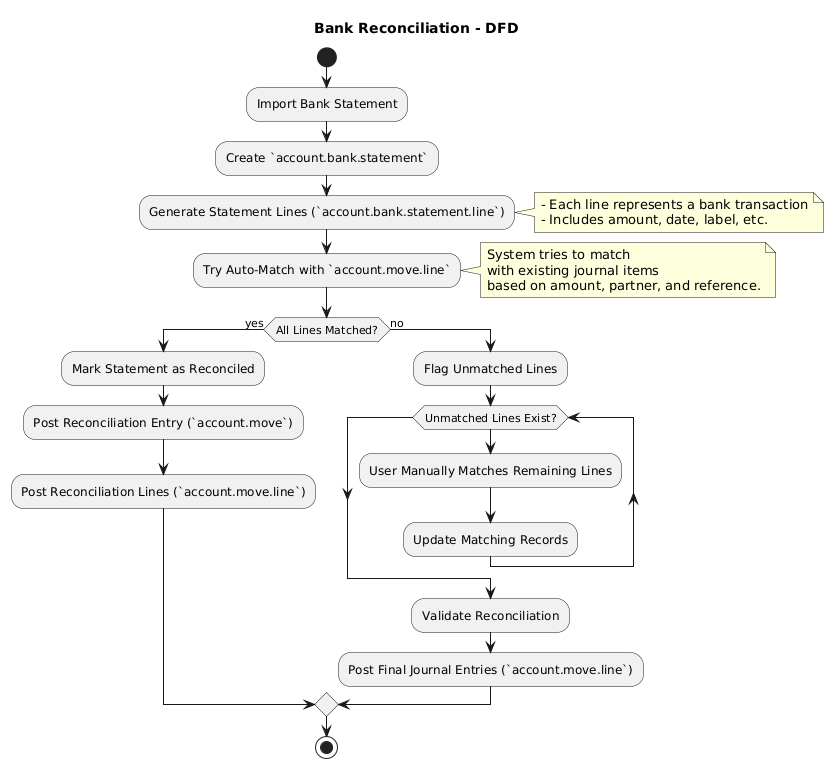
\includegraphics[width=0.8\linewidth]{diagram/bankreconciliation-DFD.png}
\end{center}

\noindent\textbf{Purpose:} Imagines matching bank statement lines to accounting records.
\medskip

\noindent\textbf{Steps:}

\noindent -Import Bank Statement (account.bank.statement): Bank statements are imported.

\noindent -Create Statement Lines (account.bank.statement.line): Each transaction is split into lines.

\noindent -Match with Invoices (account.move.line): The system suggests matches with unpaid invoices.

\noindent -Validate Reconciliation (account.move): Reconciliation is validated.

\noindent -Post Journal Entries (account.move.line): Final accounting postings are posted if needed.

\newpage
\section{Odoo Features and Customization}
\subsection{Odoo UI \& UX for Accounting}

Odoo's user interface (UI) and user experience (UX) for the Accounting module are designed to 
be intuitive and efficient, providing users with easy access to financial data and tools. Here's an 
overview:
\medskip

\noindent\textbf{List/Form/Kanban Views for Financial Records:}
\begin{center}
    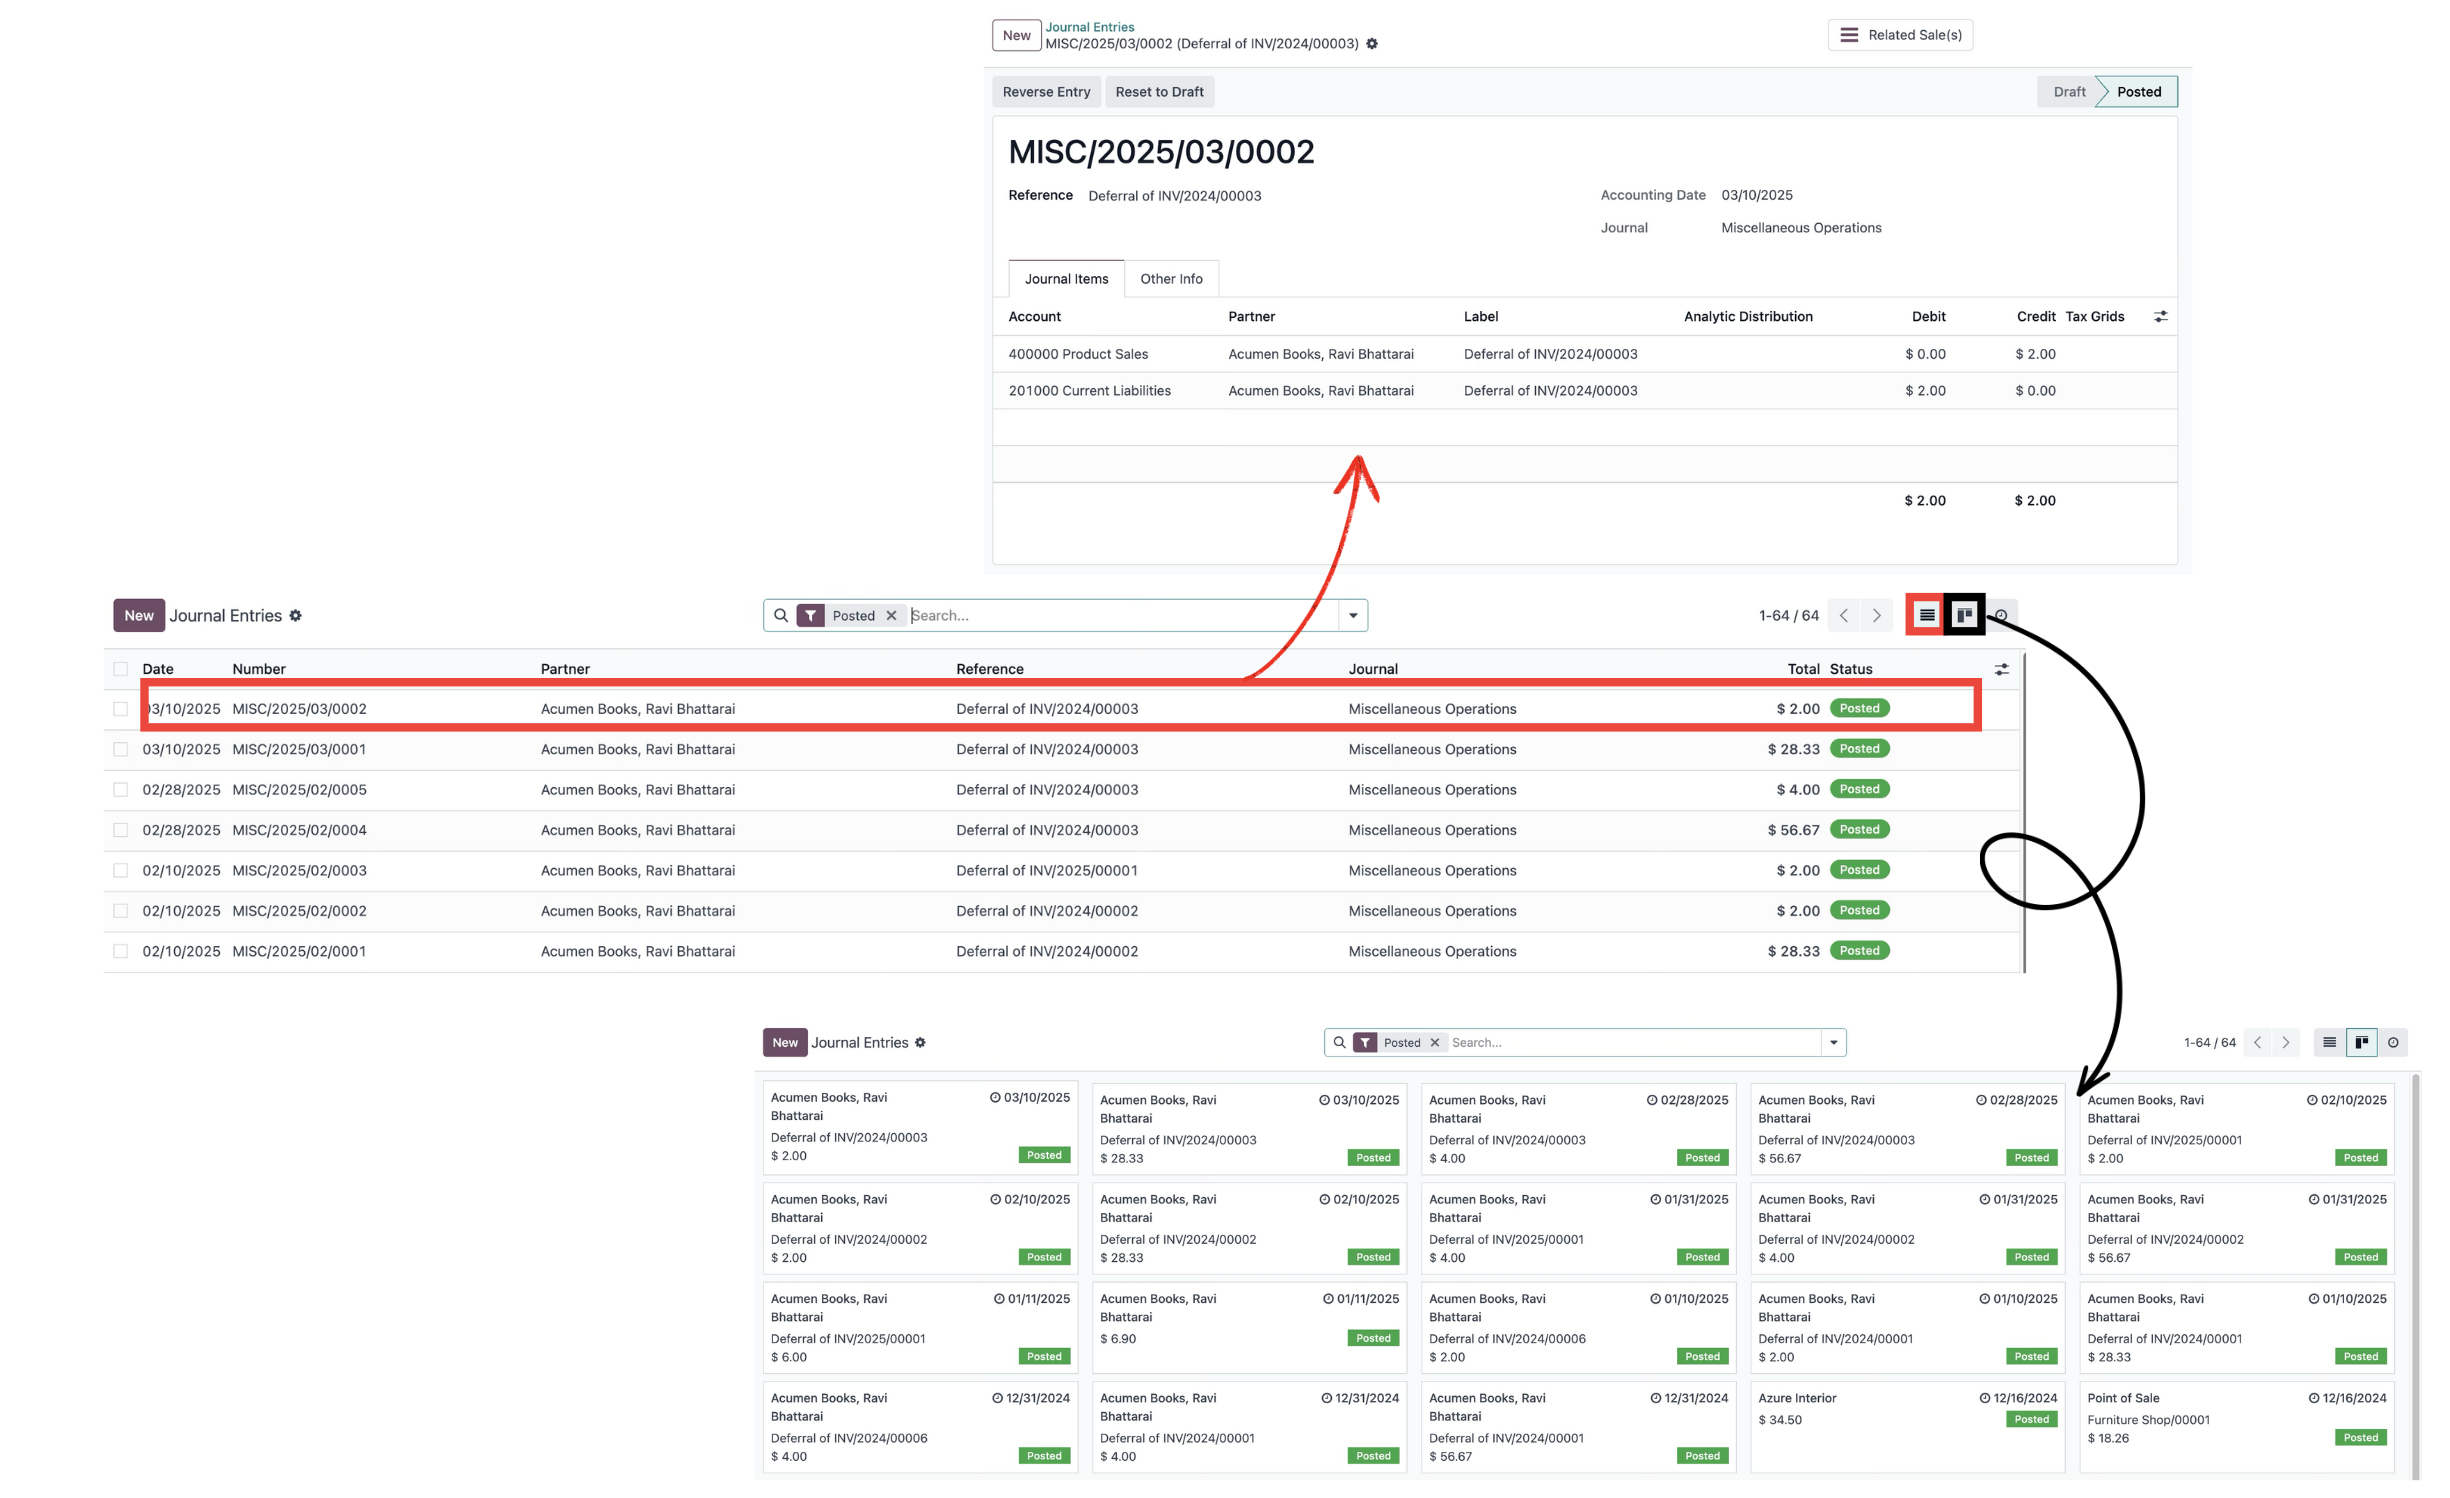
\includegraphics[width=0.8\linewidth]{diagram/UI_one.png}
\end{center}

\noindent\textbf{List View:} Provides a tabular display of records, allowing users to quickly scan and sort data. 
This view is commonly used for journal entries, invoices, bills, and payments.
\medskip

\noindent\textbf{Form View:} Displays detailed information for a single record, allowing users to edit and update 
data. This view is used for creating and modifying journal entries, invoices, bills, payments, and 
other financial records.
\medskip

\noindent\textbf{Kanban View:} Presents records as cards in columns, allowing users to visually track the 
progress of financial processes. This view can be used for managing invoices, bills, and 
payments.
\bigskip

\noindent\textbf{Filters and Groupings for Reports:}
\begin{center}
    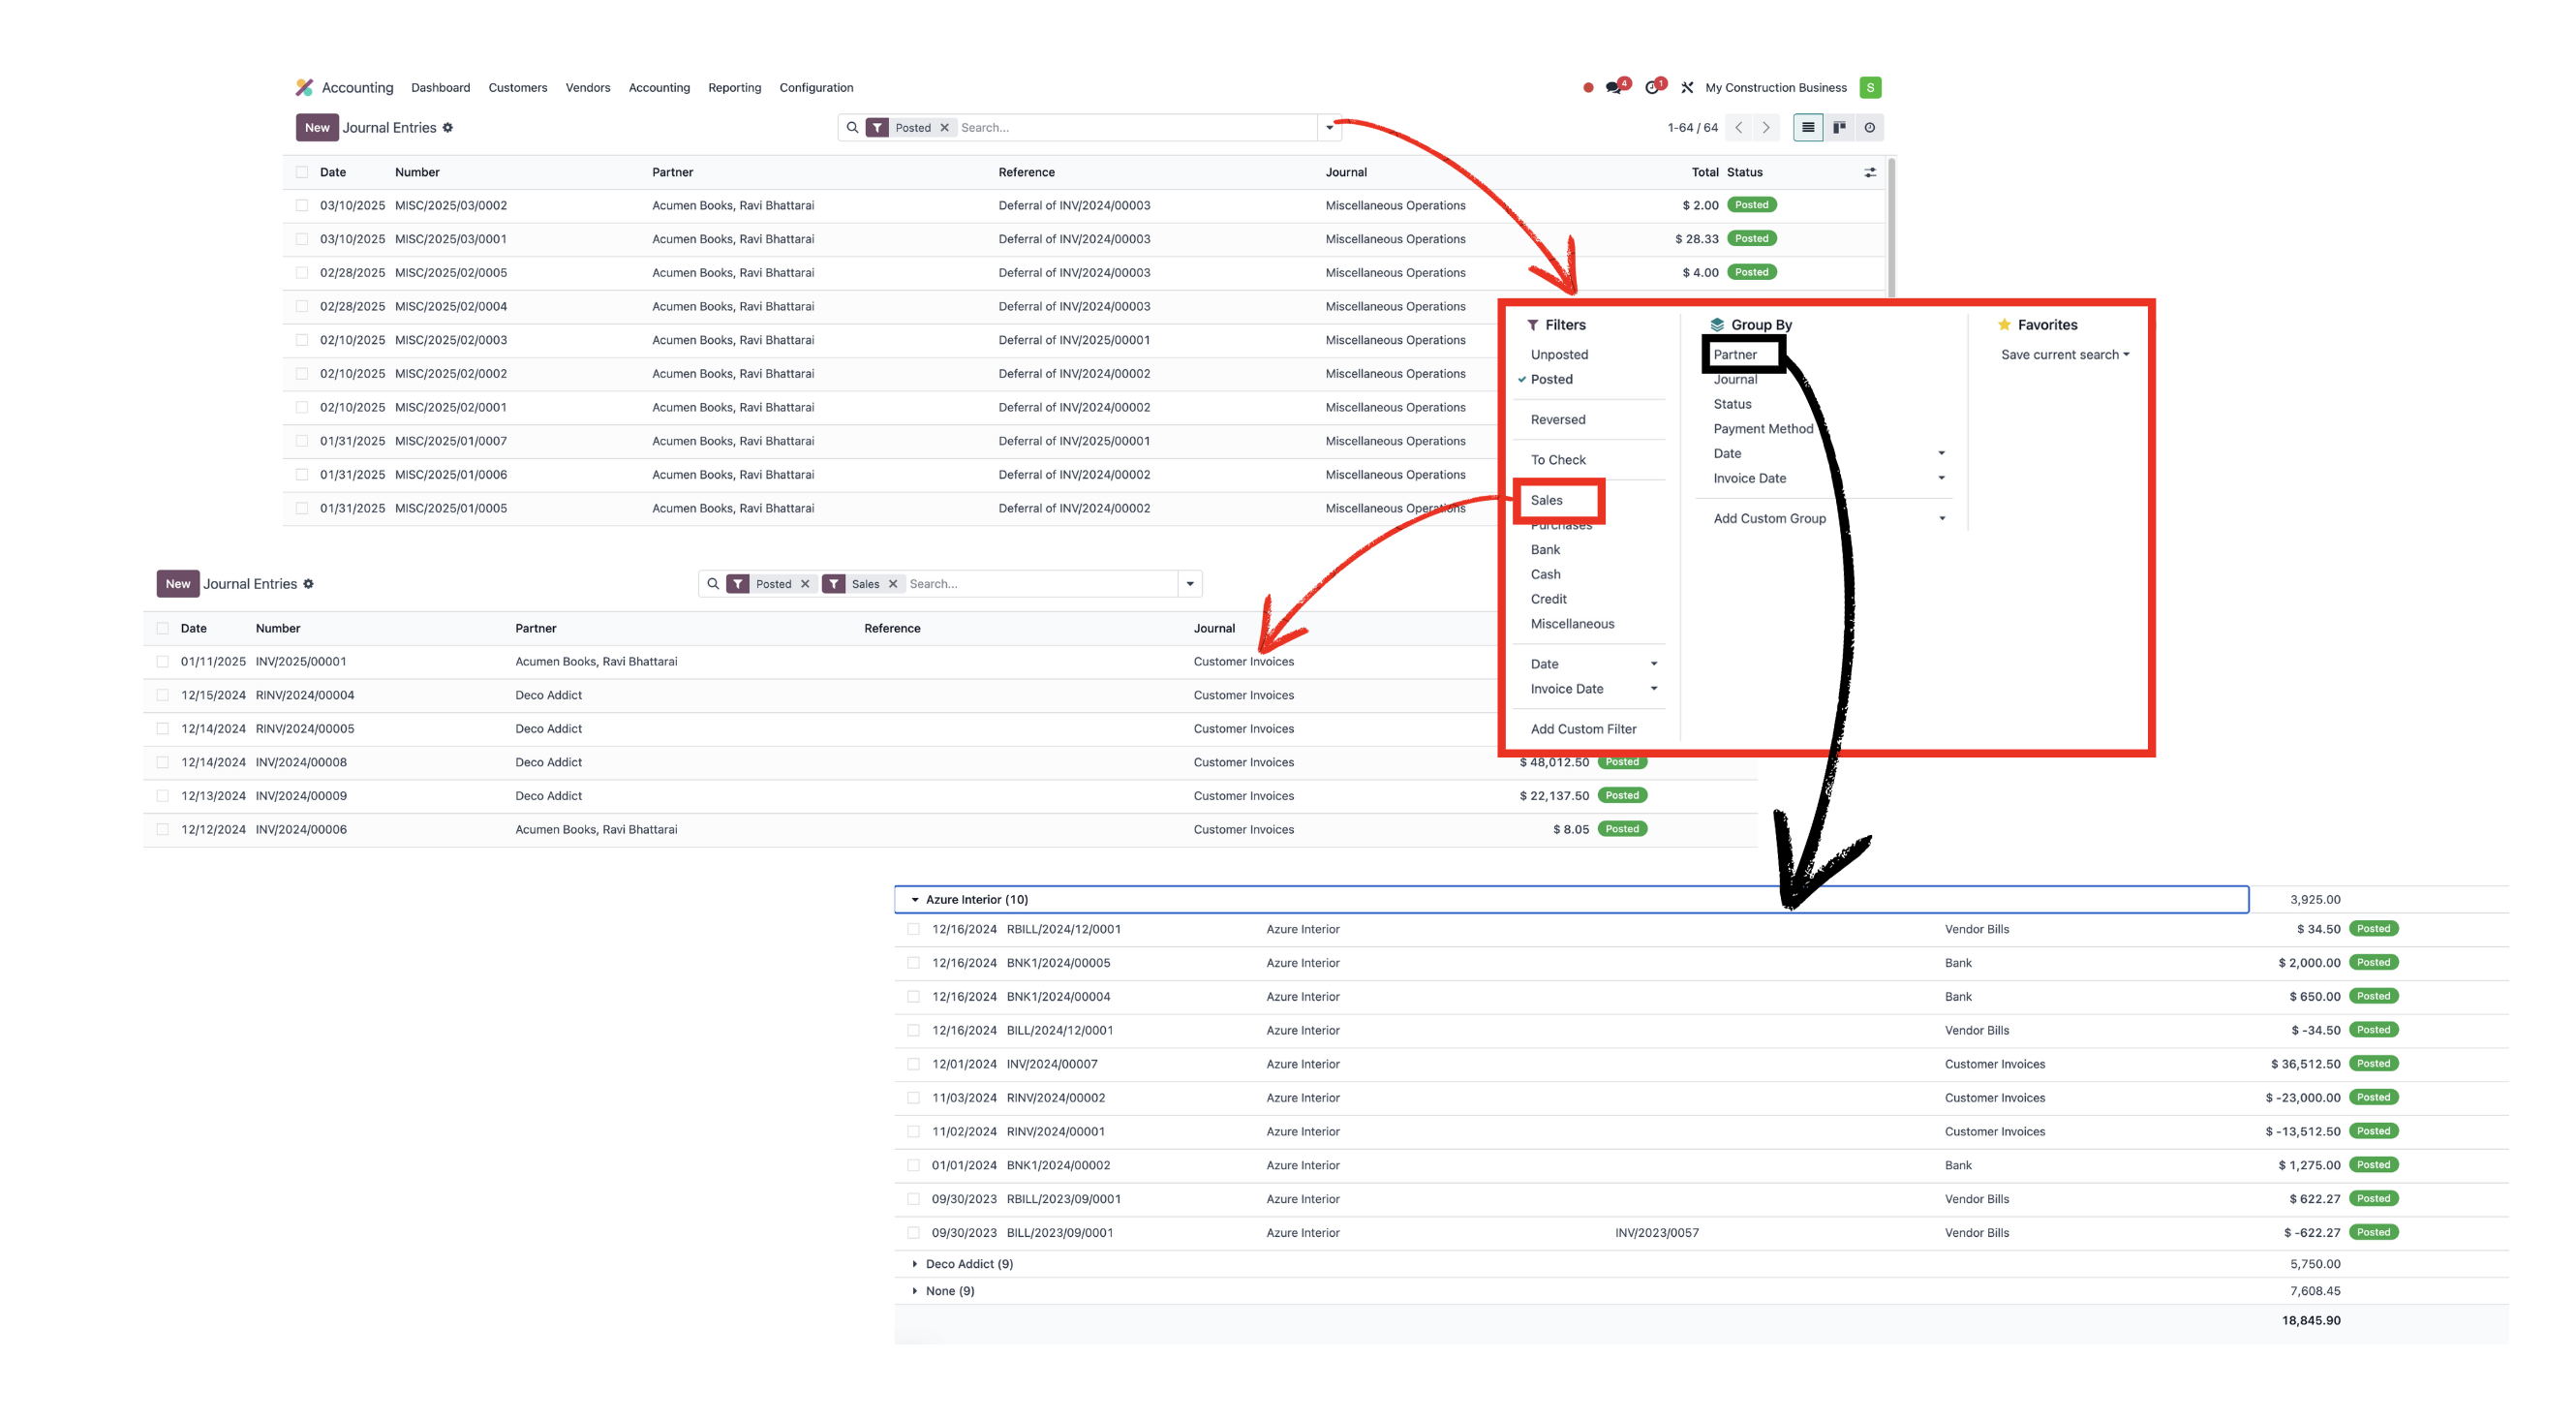
\includegraphics[width=0.8\linewidth]{diagram/UI_two.png}
\end{center}

\noindent\textbf{Filters:} Allow users to narrow down the data displayed in reports based on specific criteria (e.g., 
date range, customer, product).
\medskip

\noindent\textbf{Groupings:} Allow users to aggregate data in reports based on specific fields (e.g., by customer, 
by product, by month).

\subsection{Configuration Options}

\noindent The Odoo Accounting module comes with enormous configurations to enable the system to suit 
your requirements in your business and remain compliant with accounting standards and 
regulations. Take a look at the overview below:
\bigskip

\noindent\textbf{Chart of Accounts:}
\begin{center}
    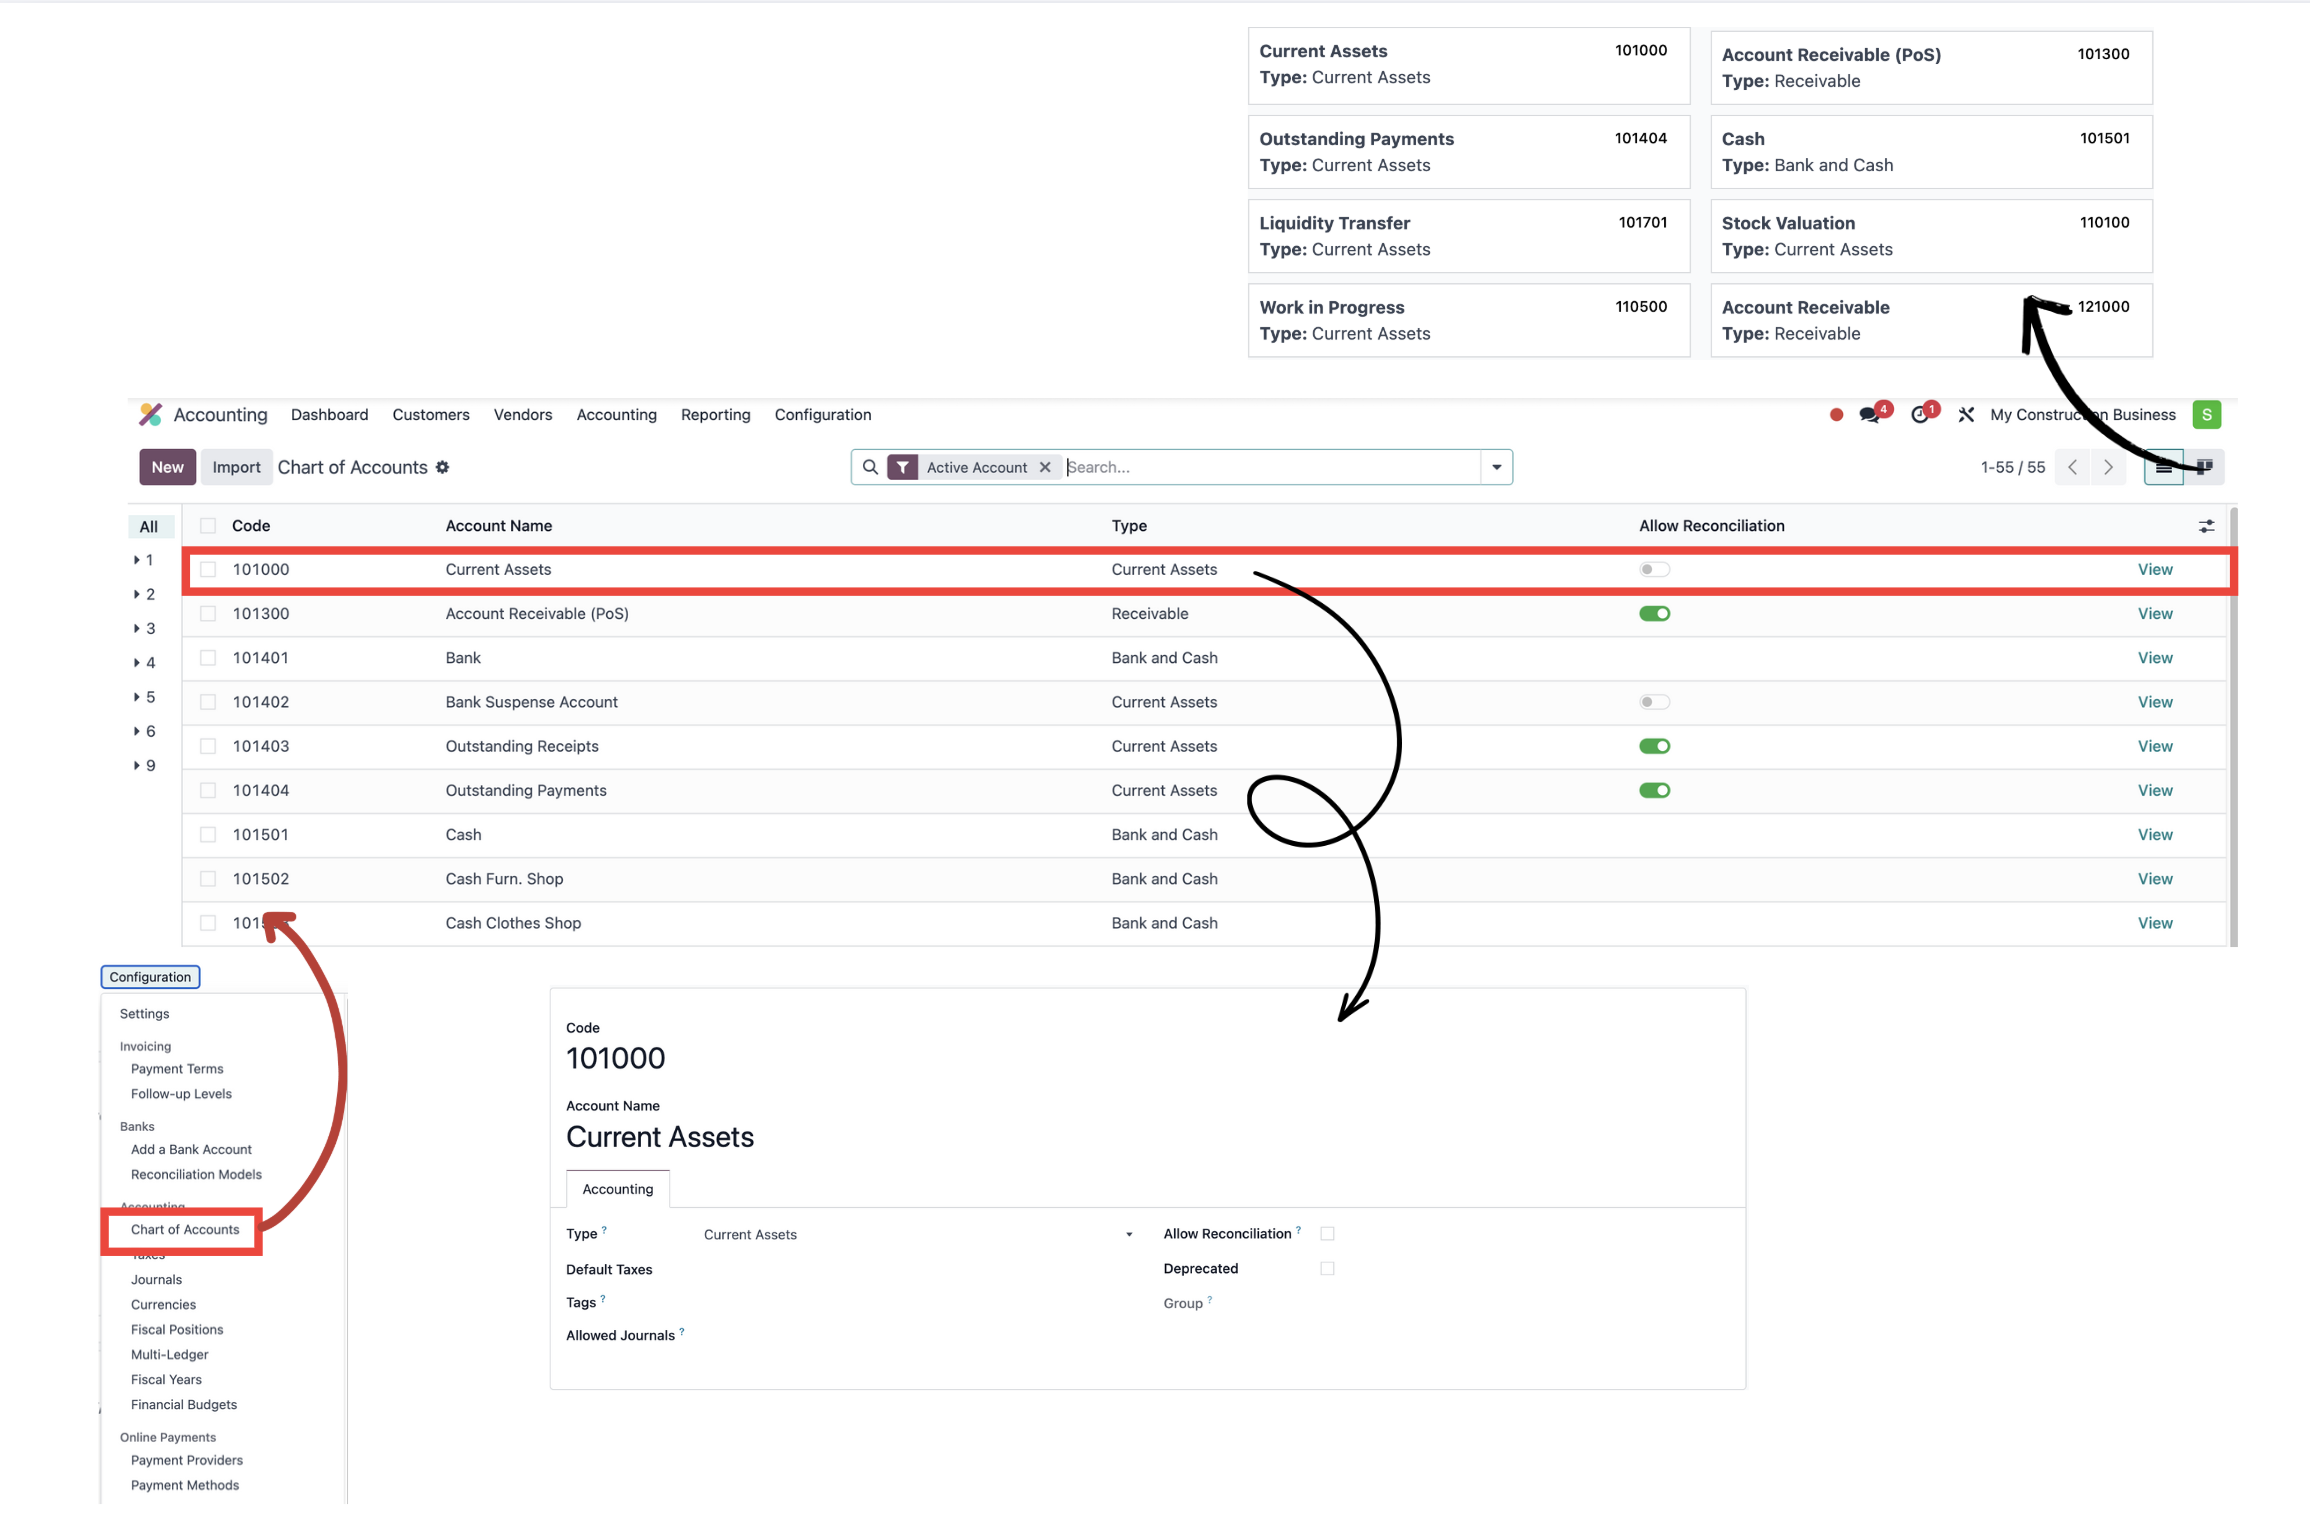
\includegraphics[width=0.8\linewidth]{diagram/COA.png}
\end{center}

\noindent\textbf{Configuration:} Odoo allows you to create your chart of accounts so you can break down the 
account which you utilized in recording fiscal transactions. New accounts can be created, edit or 
alter existing accounts can be specified through account types.
\medskip

\noindent\textbf{Best Practices:}
\begin{enumerate}
    \item Start with a typical chart of accounts (e.g., US GAAP, IFRS).
    \item Tailor the chart of accounts to your own business needs.
    \item Assign each account with a classification and linked type of account.
\end{enumerate}

\newpage
\noindent\textbf{Taxes and Fiscal Positions:}
\begin{center}
    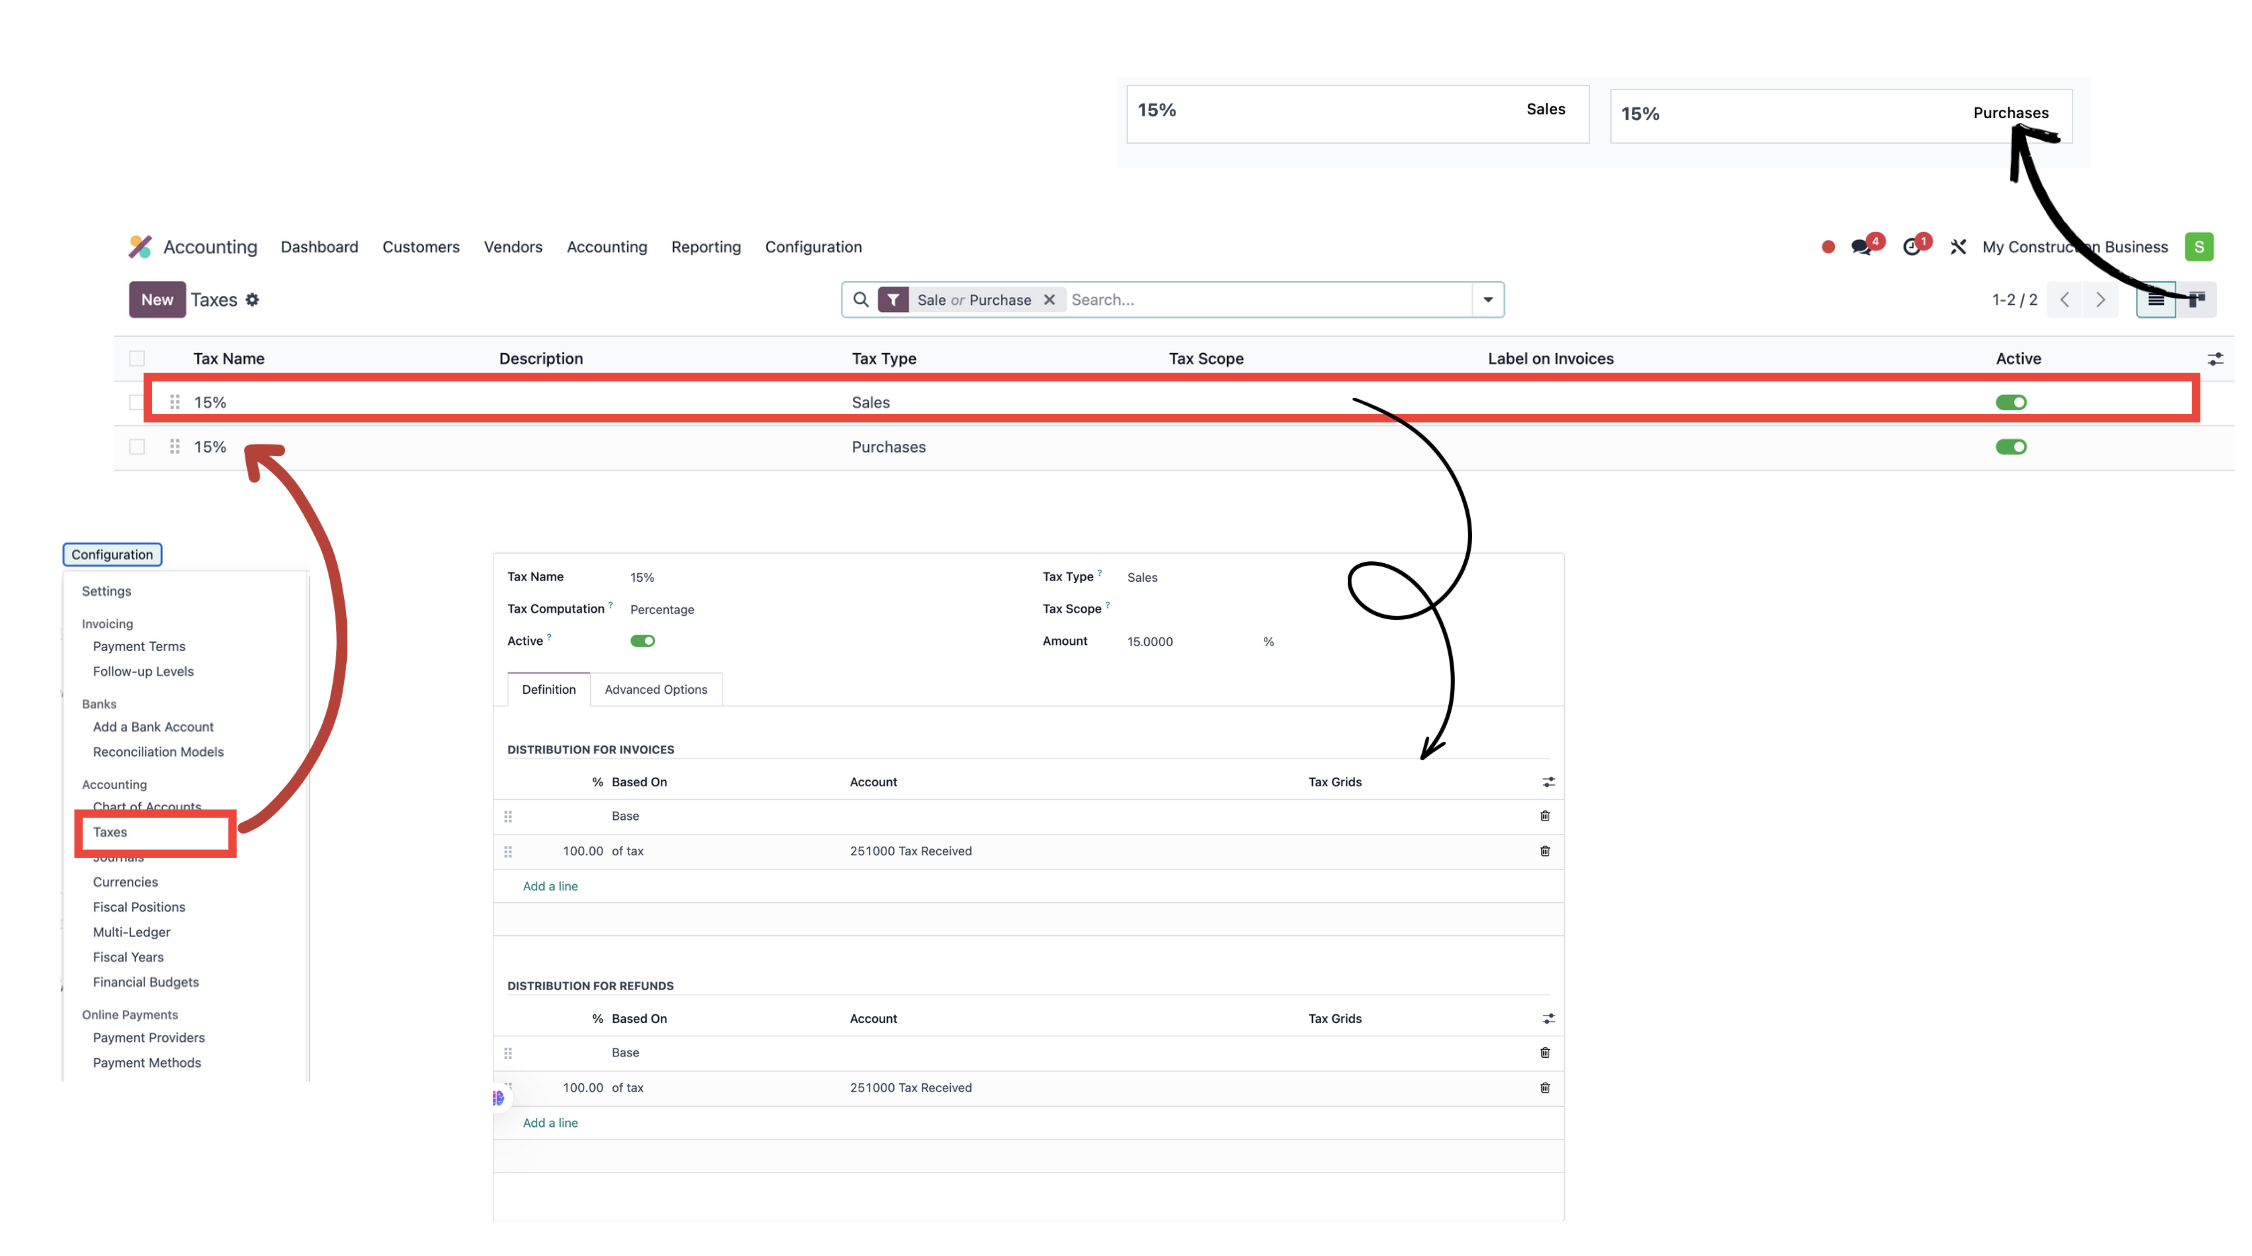
\includegraphics[width=0.8\linewidth]{diagram/Taxes.png}
    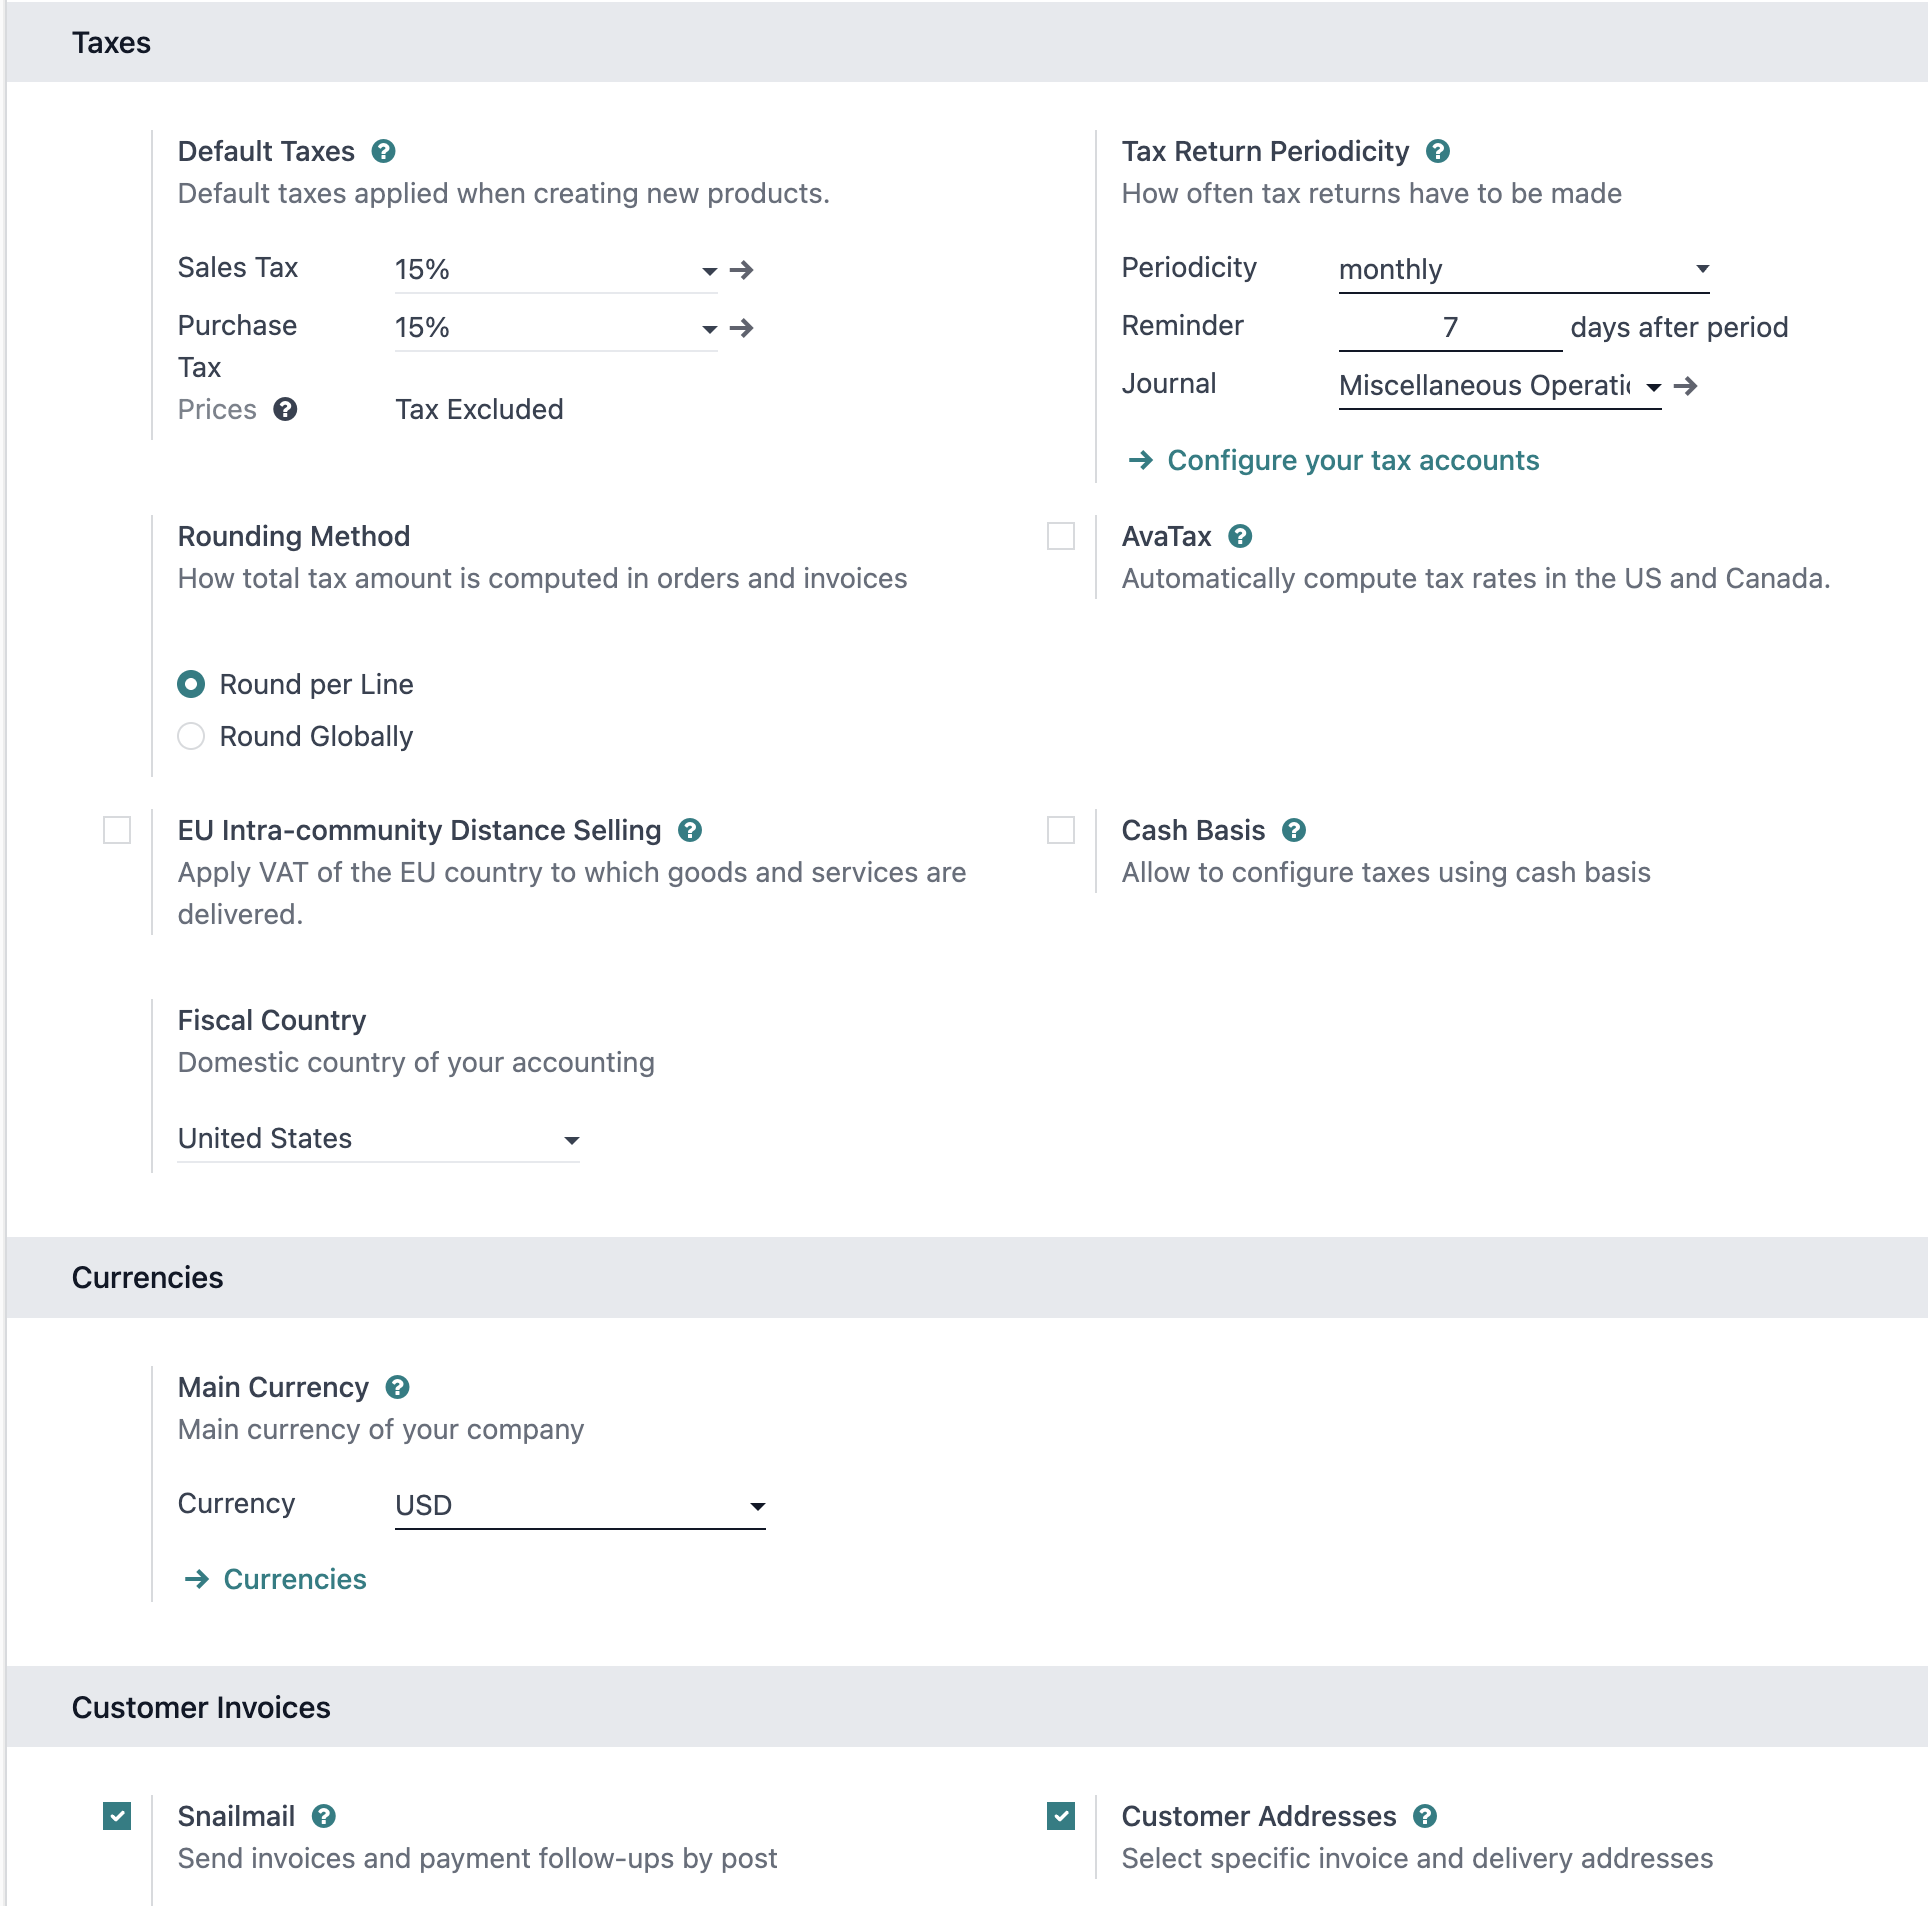
\includegraphics[width=0.8\linewidth]{diagram/Taxes_second.png}
\end{center}

\noindent\textbf{Configuration:} Odoo allows you to set up taxes and fiscal positions, specifying the tax regulations for 
specific transactions based on the involved parties.
\medskip

\noindent\textbf{Best Practices:}
\begin{enumerate}
    \item Define all applicable taxes and tax rates.
    \item Set fiscal positions for different customer and supplier locations.
    \item Ensure tax rules are correctly configured to comply with tax regulations.
\end{enumerate}

\newpage
\noindent\textbf{Multi-Currency and Exchange Rates:}
\begin{center}
    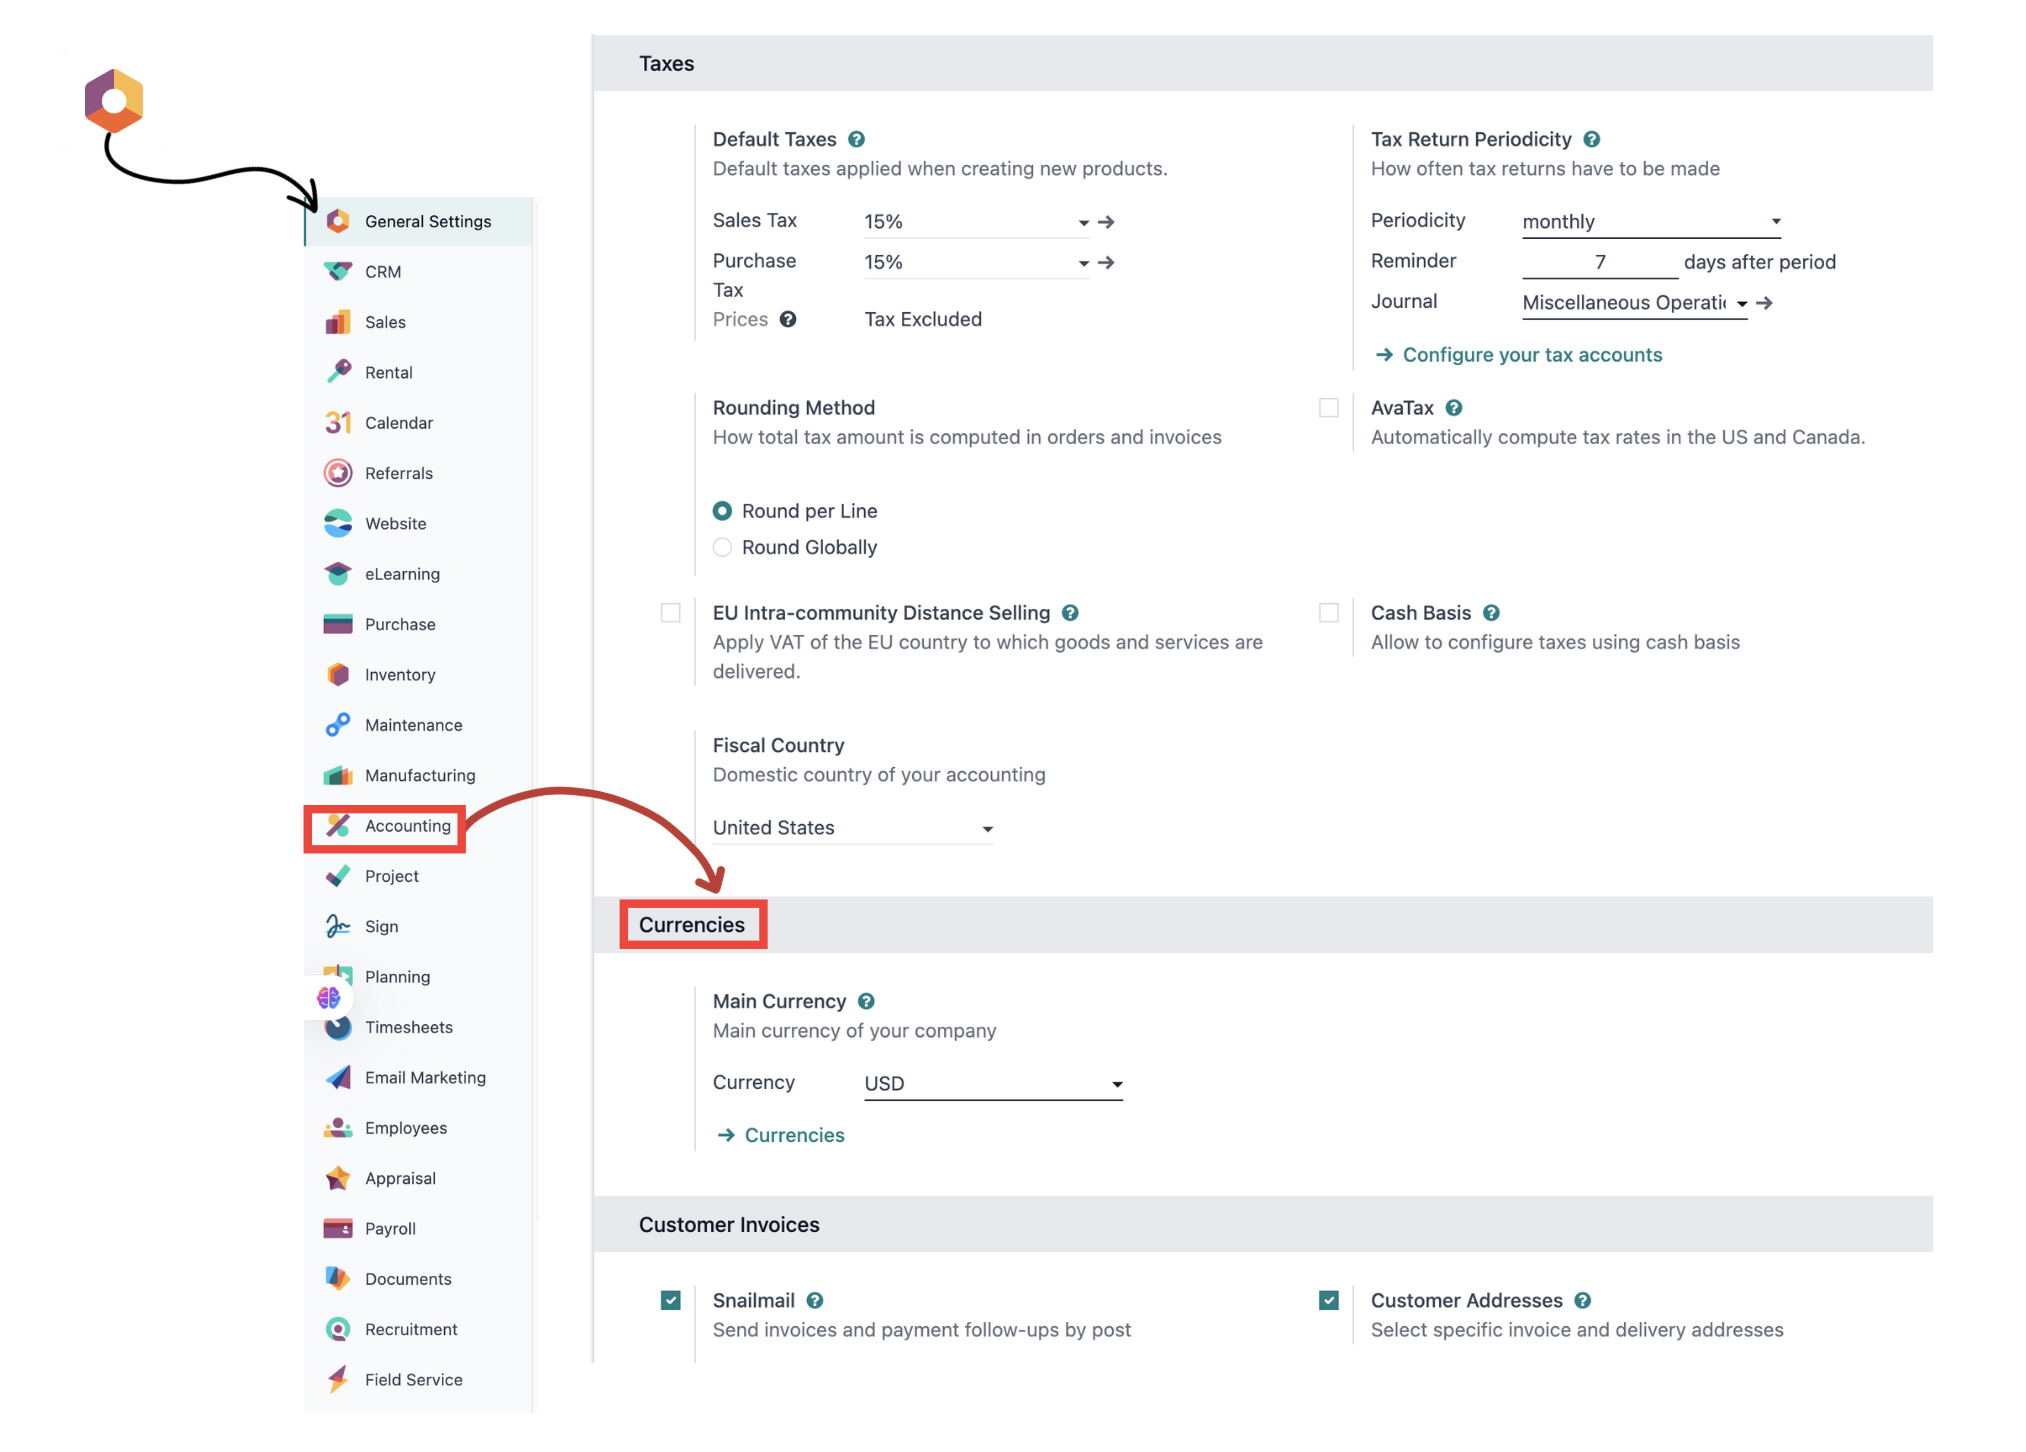
\includegraphics[width=0.8\linewidth]{diagram/Currency.png}
\end{center}

\noindent\textbf{Configuration:} Odoo supports multi-currency accounting, where you can conduct transactions in 
different currencies. You can configure exchange rates and automatically update exchange rates.
\medskip

\noindent\textbf{Best Practices:}
\begin{enumerate}
    \item Enable multi-currency functionality if you operate in different currencies.
    \item Automatically update exchange rates to ensure proper currency conversions.
    \item Manually check and update exchange rates at intervals.
\end{enumerate}

\newpage
\noindent\textbf{Company Setup (Fiscal Years, Lock Dates):}
\begin{center}
    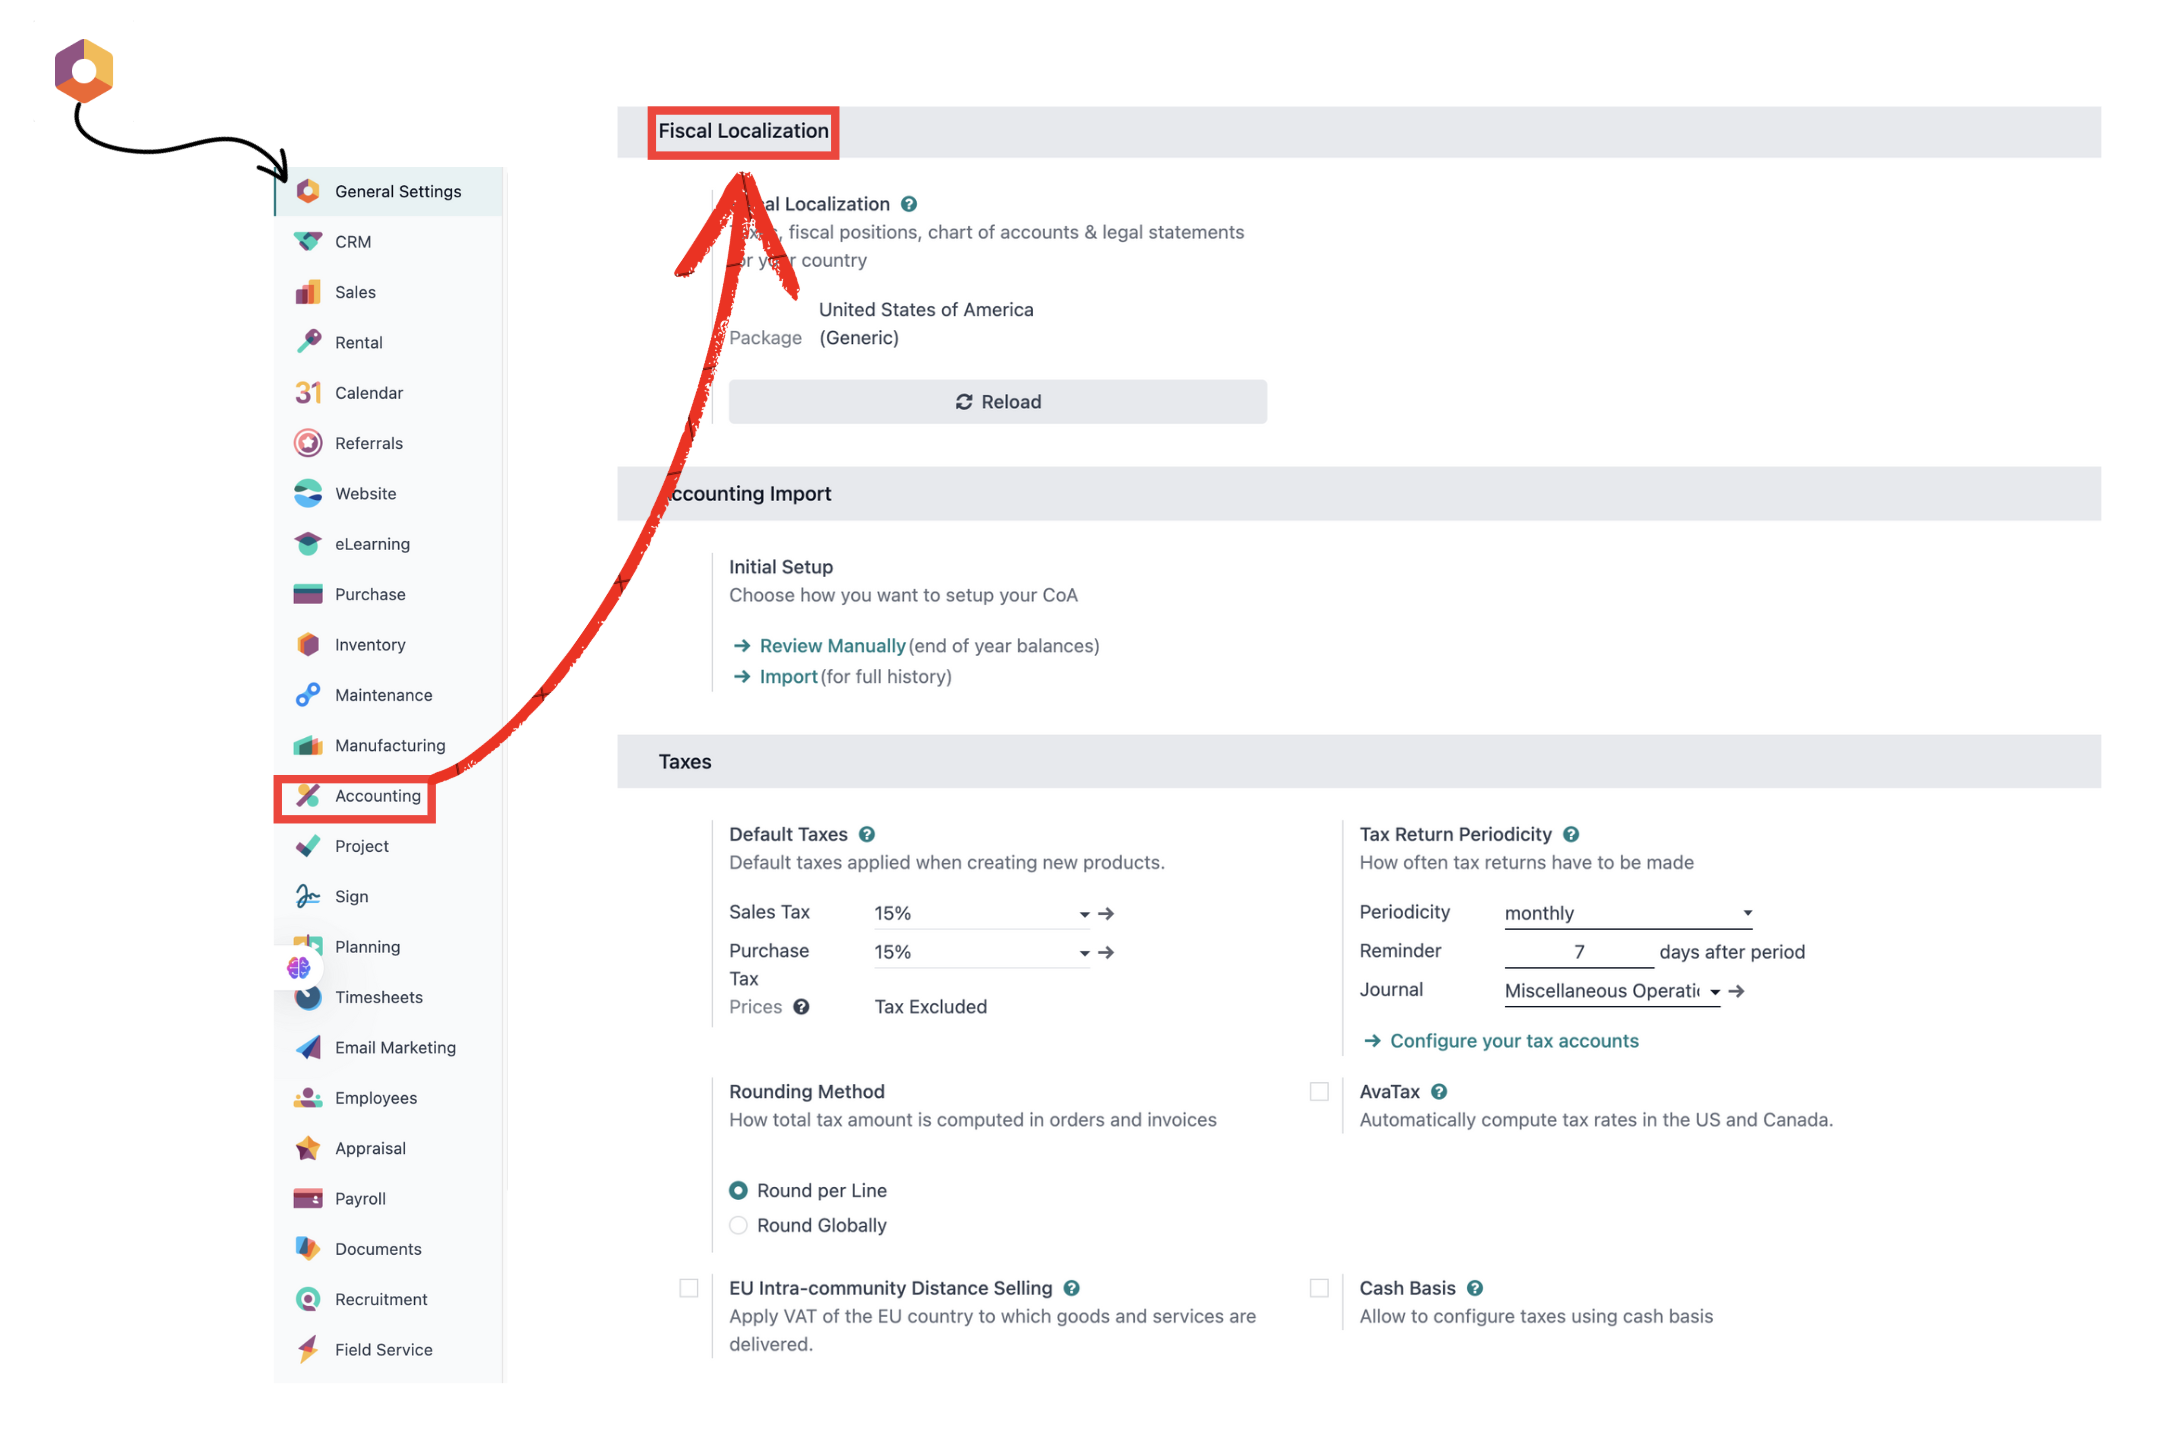
\includegraphics[width=0.8\linewidth]{diagram/Fiscal_Localization.png}
    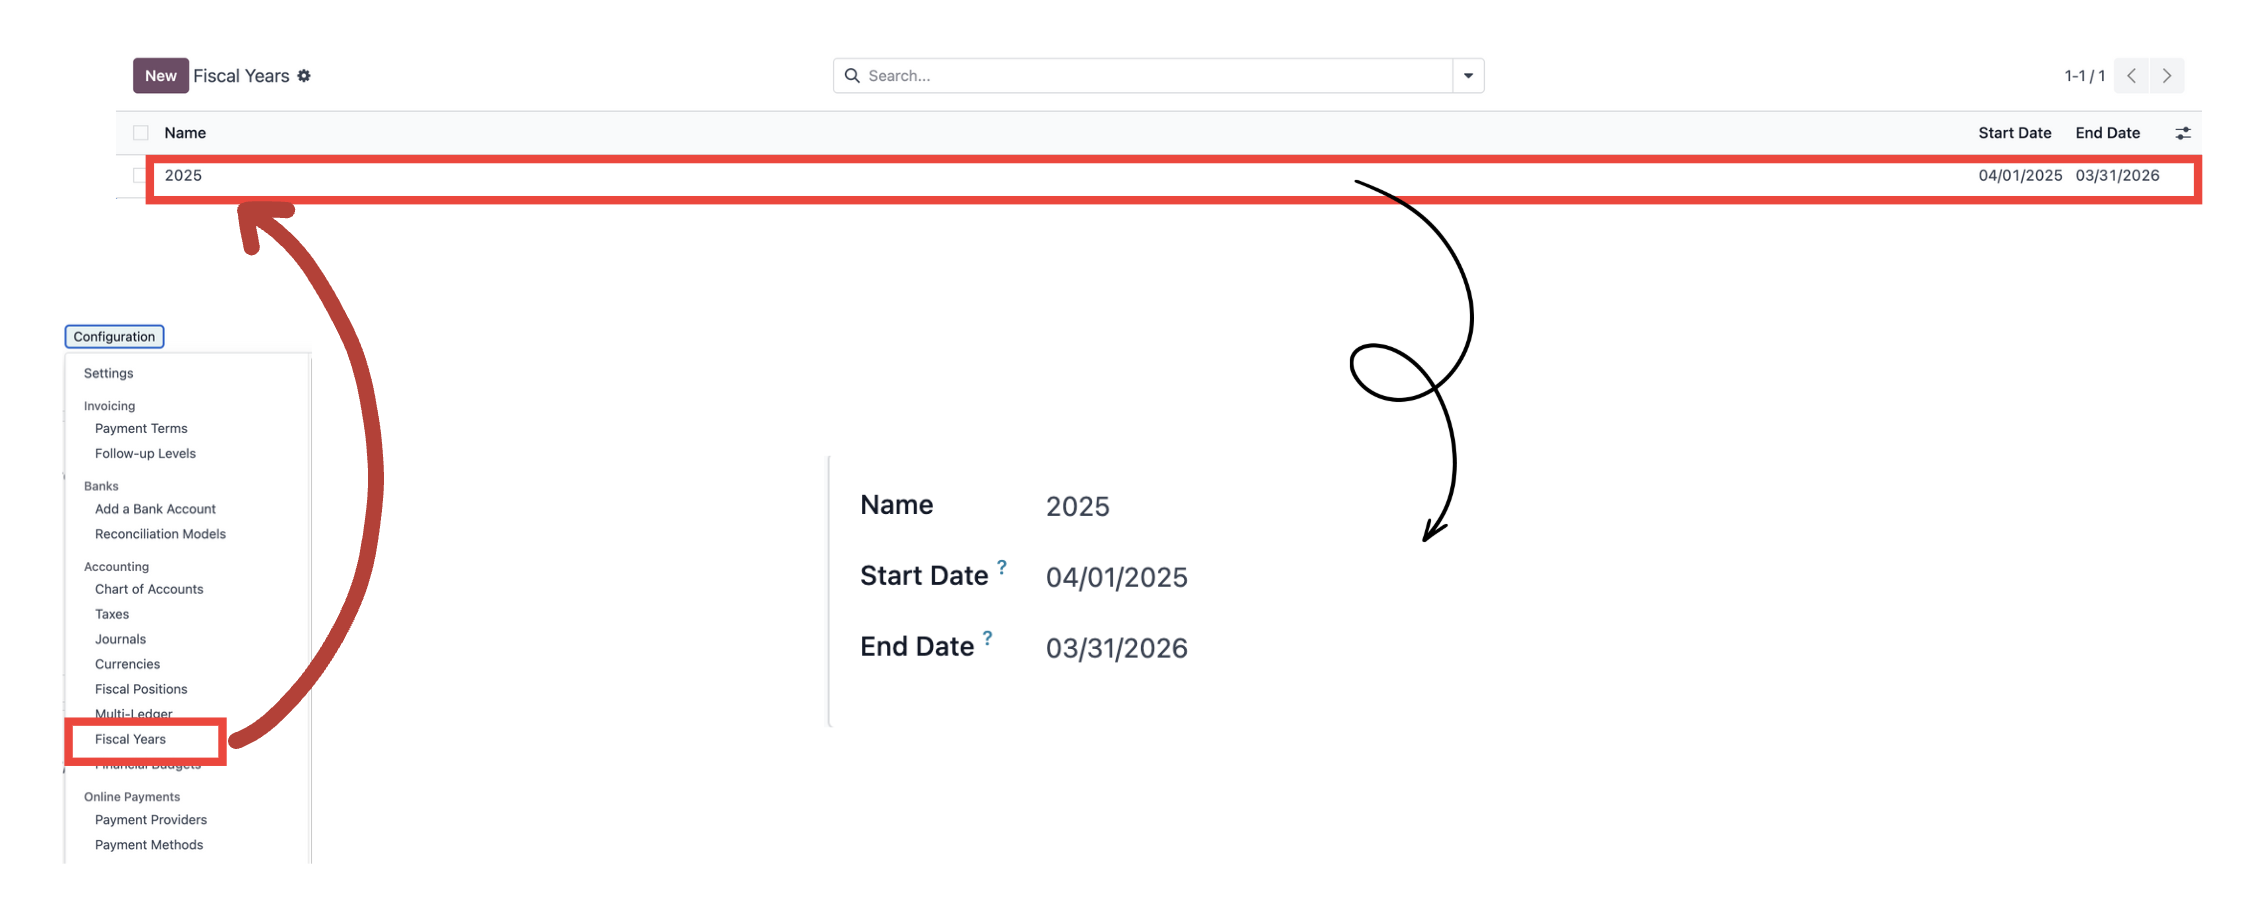
\includegraphics[width=0.8\linewidth]{diagram/Fiscal_year.png}
\end{center}

\noindent\textbf{Configuration:} Odoo allows you to define fiscal years and lock dates, which define the years for which 
financial statements are to be prepared and the dates after which no further changes may be done 
to the accounting records.
\medskip

\noindent\textbf{Best Practices:}
\begin{enumerate}
    \item Define fiscal years that correspond to your company cycle.
    \item Set lock dates to prevent unauthorized changes to accounting records.
    \item Close accounting periods on a regular schedule to offer accurate financial reporting.
\end{enumerate}

\newpage
\subsection{Customization and Development}
\subsubsection{UML for customization}
\noindent\textbf{Use Case: Custom Invoice approval process}
\begin{center}
    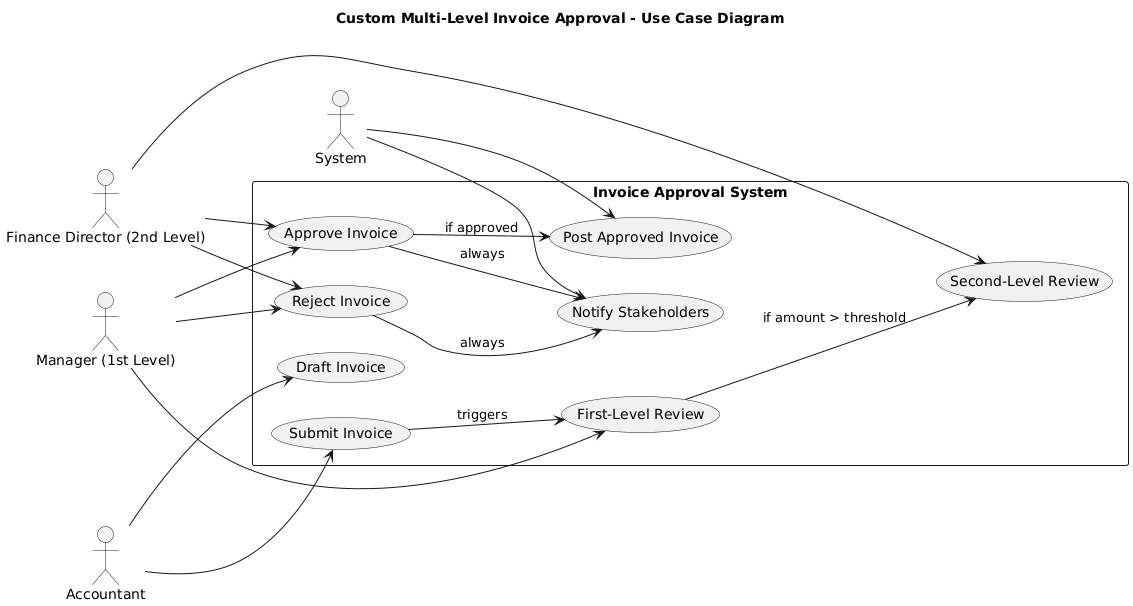
\includegraphics[width=0.8\linewidth]{diagram/custom_multi_level.png}
\end{center}

\noindent The Custom Multi-Level Invoice Approval workflow in Odoo extends the standard invoice 
workflow with formal roles and a multi-level review. It begins with the Accountant, where an 
invoice is prepared and submitted for approval. The invoice enters a First-Level Review by a 
Manager upon submission, ensuring that all the required information is accurate and complies 
with company policies. If the invoice amount is higher than a certain value or requires higher 
authorization, it goes to a Second-Level Review by the Finance Director. The Director and 
Manager can both approve or reject the invoice. Rejection must be with a reason, which is used 
by the System to notify the Accountant to take necessary action. On approval, the System 
automatically posts the invoice and makes the necessary adjustments to the accounting records.
\medskip

\noindent This setup maximizes financial control, reduces the potential for error, and ensures high-value or 
sensitive transactions are correctly scrutinized. The workflow is nicely captured in a Use Case 
UML diagram that outlines the interaction of each actor with the system, approval flow, and 
escalation and system automation criteria. This is the ideal solution for organizations that need 
accountability, audit trails, and compliance within their invoicing process.
\bigskip

\noindent\textbf{Activity Diagram: Automated bank reconciliation}

\noindent The higher-level activity diagram for bank automatic reconciliation explains an elaborate process 
through which both users and the system collaborate to match bank statements appropriately and 
with maximum efficiency. The process initiates 
with importing a bank statement after which 
the system reads and attempts to automatically 
associate transactions with pre-existing 
accounting records. A decision node checks 
whether all the transactions are successfully 
matched. If they are, the system then proceeds 
to stamp the statement as fully reconciled and 
change its status, and it stops the process.

\noindent
\begin{minipage}{0.5\textwidth}
When not all the transactions match, the 
system stamps the unmatched ones, causing a 
manual intervention step. At this step, a user—
in most cases, an accountant—scans the
unmatched transactions, matches them by hand 
or generates new records where necessary. 
Following this, a retry logic loop is triggered 
where the system tries to auto-match any 
other unmatched items again. If the items 
continue to fail matching, the system raises an 
exception and notifies the 
accountant so that unsolved items 
can be traced properly and 
escalated accordingly.
\medskip

It stops when reconciliation is 
finalized and the greatest number of 
permitted attempts at 
matching have been made. Finally, 
the system completes reconciling 
and refreshes the log of 
reconciliation to be utilized as an 
audit source. It is a sophisticated 
flow that enables greater data integrity, accountability and 
minimizes the scope of reconciliation error by finding a balance 
between auto-mation, human interaction and exception handling.
\end{minipage}%
\hfill
\begin{minipage}{0.45\textwidth}
    \centering
    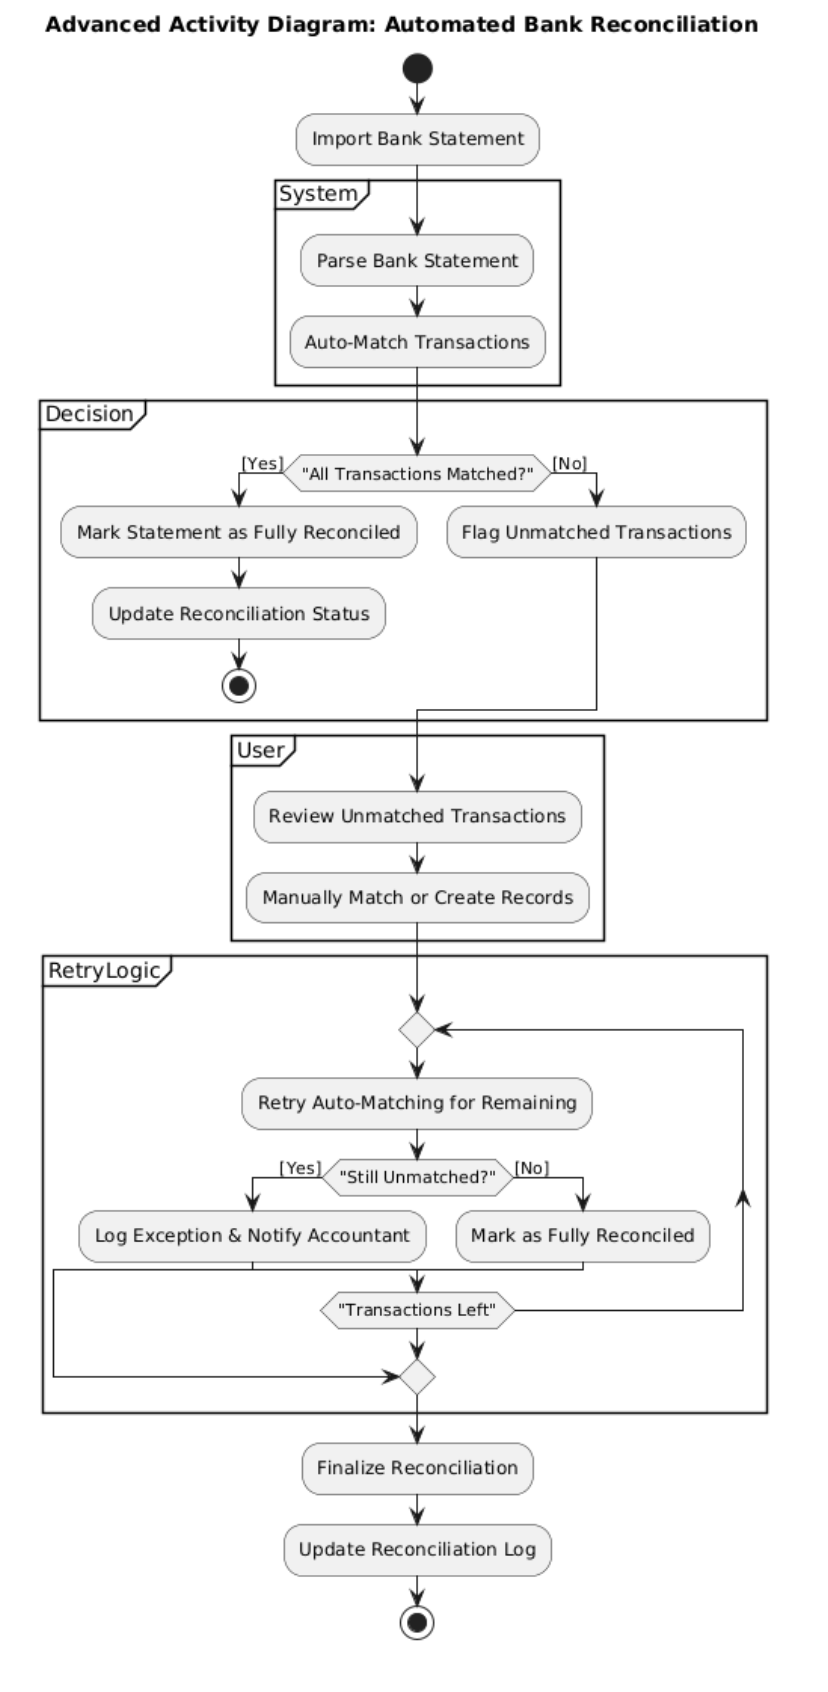
\includegraphics[width=\linewidth]{diagram/advanced_activity.png}
\end{minipage}
\bigskip

\noindent\textbf{Sequence Diagram: Invoice to Journal Posting}
\begin{center}
    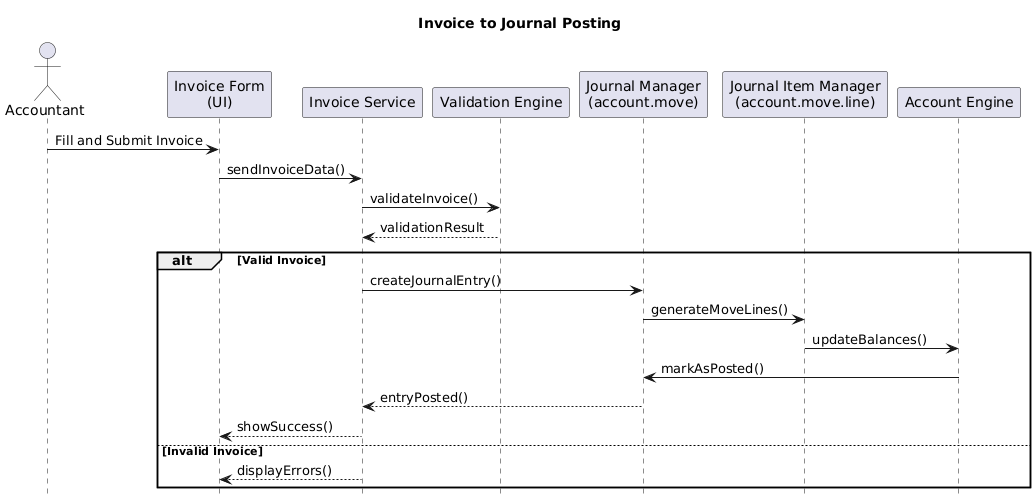
\includegraphics[width=0.8\linewidth]{diagram/Invoice to journal posting.png}
\end{center}
This advanced sequence diagram illustrates the process of posting an invoice into the accounting 
system in Odoo. It starts when an Accountant posts an invoice from the user interface, which in 
turn calls the Invoice Service to check the data through the Validation Engine. If valid, a Journal 
Entry (account.move) is created, followed by the creation of corresponding Journal Items 
(account.move.line). These postings update the account balances through the Account Engine 
and mark the journal entry as posted. If an invoice fails to validate, the user is presented with 
accurate error messages. This modular sequence ensures data consistency, transaction integrity, 
and direct feedback throughout the accounting process.

\subsubsection{Adding Analytical Dimensions}
Odoo has good flexibility to extend the data structure of the Accounting module so that 
companies can monitor certain financial data and meet certain reporting or operation needs. 
Below are some common examples of these customizations:

\begin{enumerate}
        \item \textbf{Adding Analytical Dimensions}
        
        \textbf{Purpose:} To give financial monitoring with the inclusion of dimensions such as department, project, or 
        region—beyond the default chart of accounts.
        \medskip

        \begin{minipage}{0.5\textwidth}
            \centering
            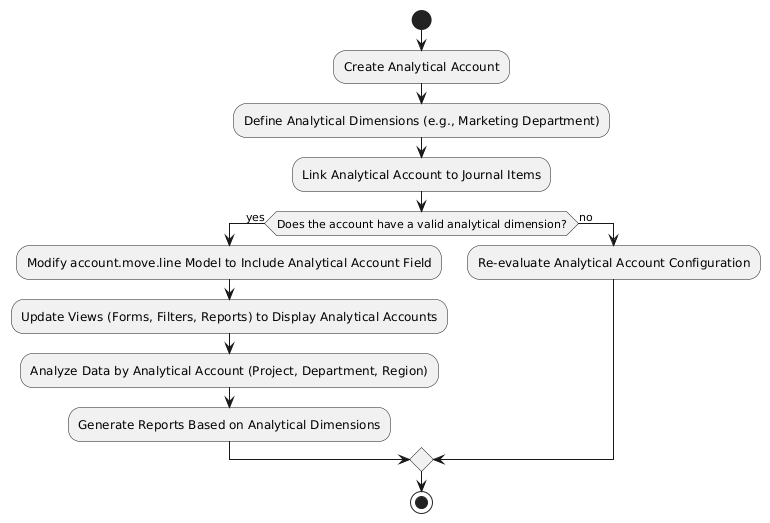
\includegraphics[width=\linewidth]{diagram/adding_analytical_dimensions.png}
        \end{minipage}%
        \hfill
        \begin{minipage}{0.45\textwidth}
                \textbf{Implementation Steps:}
                \begin{enumerate}
                    \item Create Analytical Accounts: Utilize the Analytic Accounting functionality to create analytical accounts (e.g., \"Marketing Department\" or \"Project A\").
                    \item Extend Journal Items: Add a many2one field to the account.move.line model that connects 
                    journal lines with specific analytic accounts.
                    \item Customize Views: Modify form and list views to allow users to select and show analytic accounts.
                    \item Enable Analytical Reporting: Utilize Odoo's internal reporting capabilities (or custom reports) 
                    to filter, group, and report finance data by analytic dimension.
                \end{enumerate}
        \end{minipage}

    \item \textbf{Customizing Tax Fields or Journals}
    \begin{enumerate}
        \item \textbf{Custom Tax Fields}
        \medskip
        \textbf{Purpose:} 
        
        Save additional information relating to tax reporting such as regulatory codes or reporting 
        categories.
        \medskip

        \textbf{Implementation Steps:}
        \begin{enumerate}
            \item Extend account.tax: Add custom fields (e.g., x\_tax\_code, x\_reporting\_category) to the account.tax model with Odoo Studio or custom modules.
            \item Modify Views: Modify tax configuration views so that users can manage these new fields.
            \item Adjust Tax Logic: Depending on the requirement, modify the tax calculation or report logic to incorporate new field values.
        \end{enumerate}

        \item \textbf{Custom Journals}
        \medskip
        \textbf{Purpose:} 
        
        To divide and process specific types of financial entries, such as payroll or grants.
        \medskip

        \textbf{Implementation Steps:}
        \begin{enumerate}
            \item Create a Journal: Navigate to Accounting > Configuration > Journals and create a new journal (e.g., "Payroll Journal").
            \item Define Journal Type and Sequence: Establish the journal type (e.g., General, Sale, Purchase) and specify an entry sequence for sequential numbering.
            \item Set up Journal Behavior: Establish default accounts, tax setups, and analytic setups as required to minimize data entry and enhance reporting.
        \end{enumerate}

    \end{enumerate}

    \end{enumerate}

\subsubsection{Odoo ORM and Python}
Odoo's Object-Relational Mapping (ORM) and Python give limitless flexibility to add and tailor 
the business logic of the Accounting module. Using these tools, you can develop custom 
behavior, automate tasks, and tailor procedures according to your business needs. Some 
instances of utilizing these tools for sophisticated customizations are described below:
\medskip

\noindent\textbf{Auto-Posting of Entries Based on Rules}
\textbf{Purpose:} Automate the automatic generation and posting of journal entries 
in Odoo, according to some predefined business rules or conditions.
\medskip

\begin{minipage}{0.55\textwidth}
\begin{enumerate}
    \item \textbf{Create a Python Method for Auto-Posting}

    A Python method will be created in the respective Odoo model 
    (typically, the \texttt{account.move} or \texttt{account.move.line} model) to 
    define the rules under which entries are to be posted automatically.
    \begin{enumerate}
        \item \textbf{Specify Conditions:} The method will set conditions such as 
        specific types of journals, transaction value thresholds, or posting dates 
        to determine when entries should be posted automatically.
        
        \item \textbf{Set up Journal Entries:} If conditions are met, the method 
        will create new \texttt{account.move} and \texttt{account.move.line} records 
        based on predefined configurations.
        
        \item \textbf{Post Journal Entries:} Finally, the method will automatically 
        post the entries, ensuring the accounting records are up to date.
    \end{enumerate}

    \item \textbf{Automate the Python Method:}
    
    Once the Python method has been written, it must be automated through a server action or a scheduled action.
    \begin{enumerate}
        \item A scheduled action may call the method at a specific interval (e.g., daily or monthly).
        \item A server action can execute the method based on specific events, such as when a new invoice or sale order is created.
    \end{enumerate}
\end{enumerate}

\end{minipage}%
\hfill
\begin{minipage}{0.45\textwidth}
    \centering
    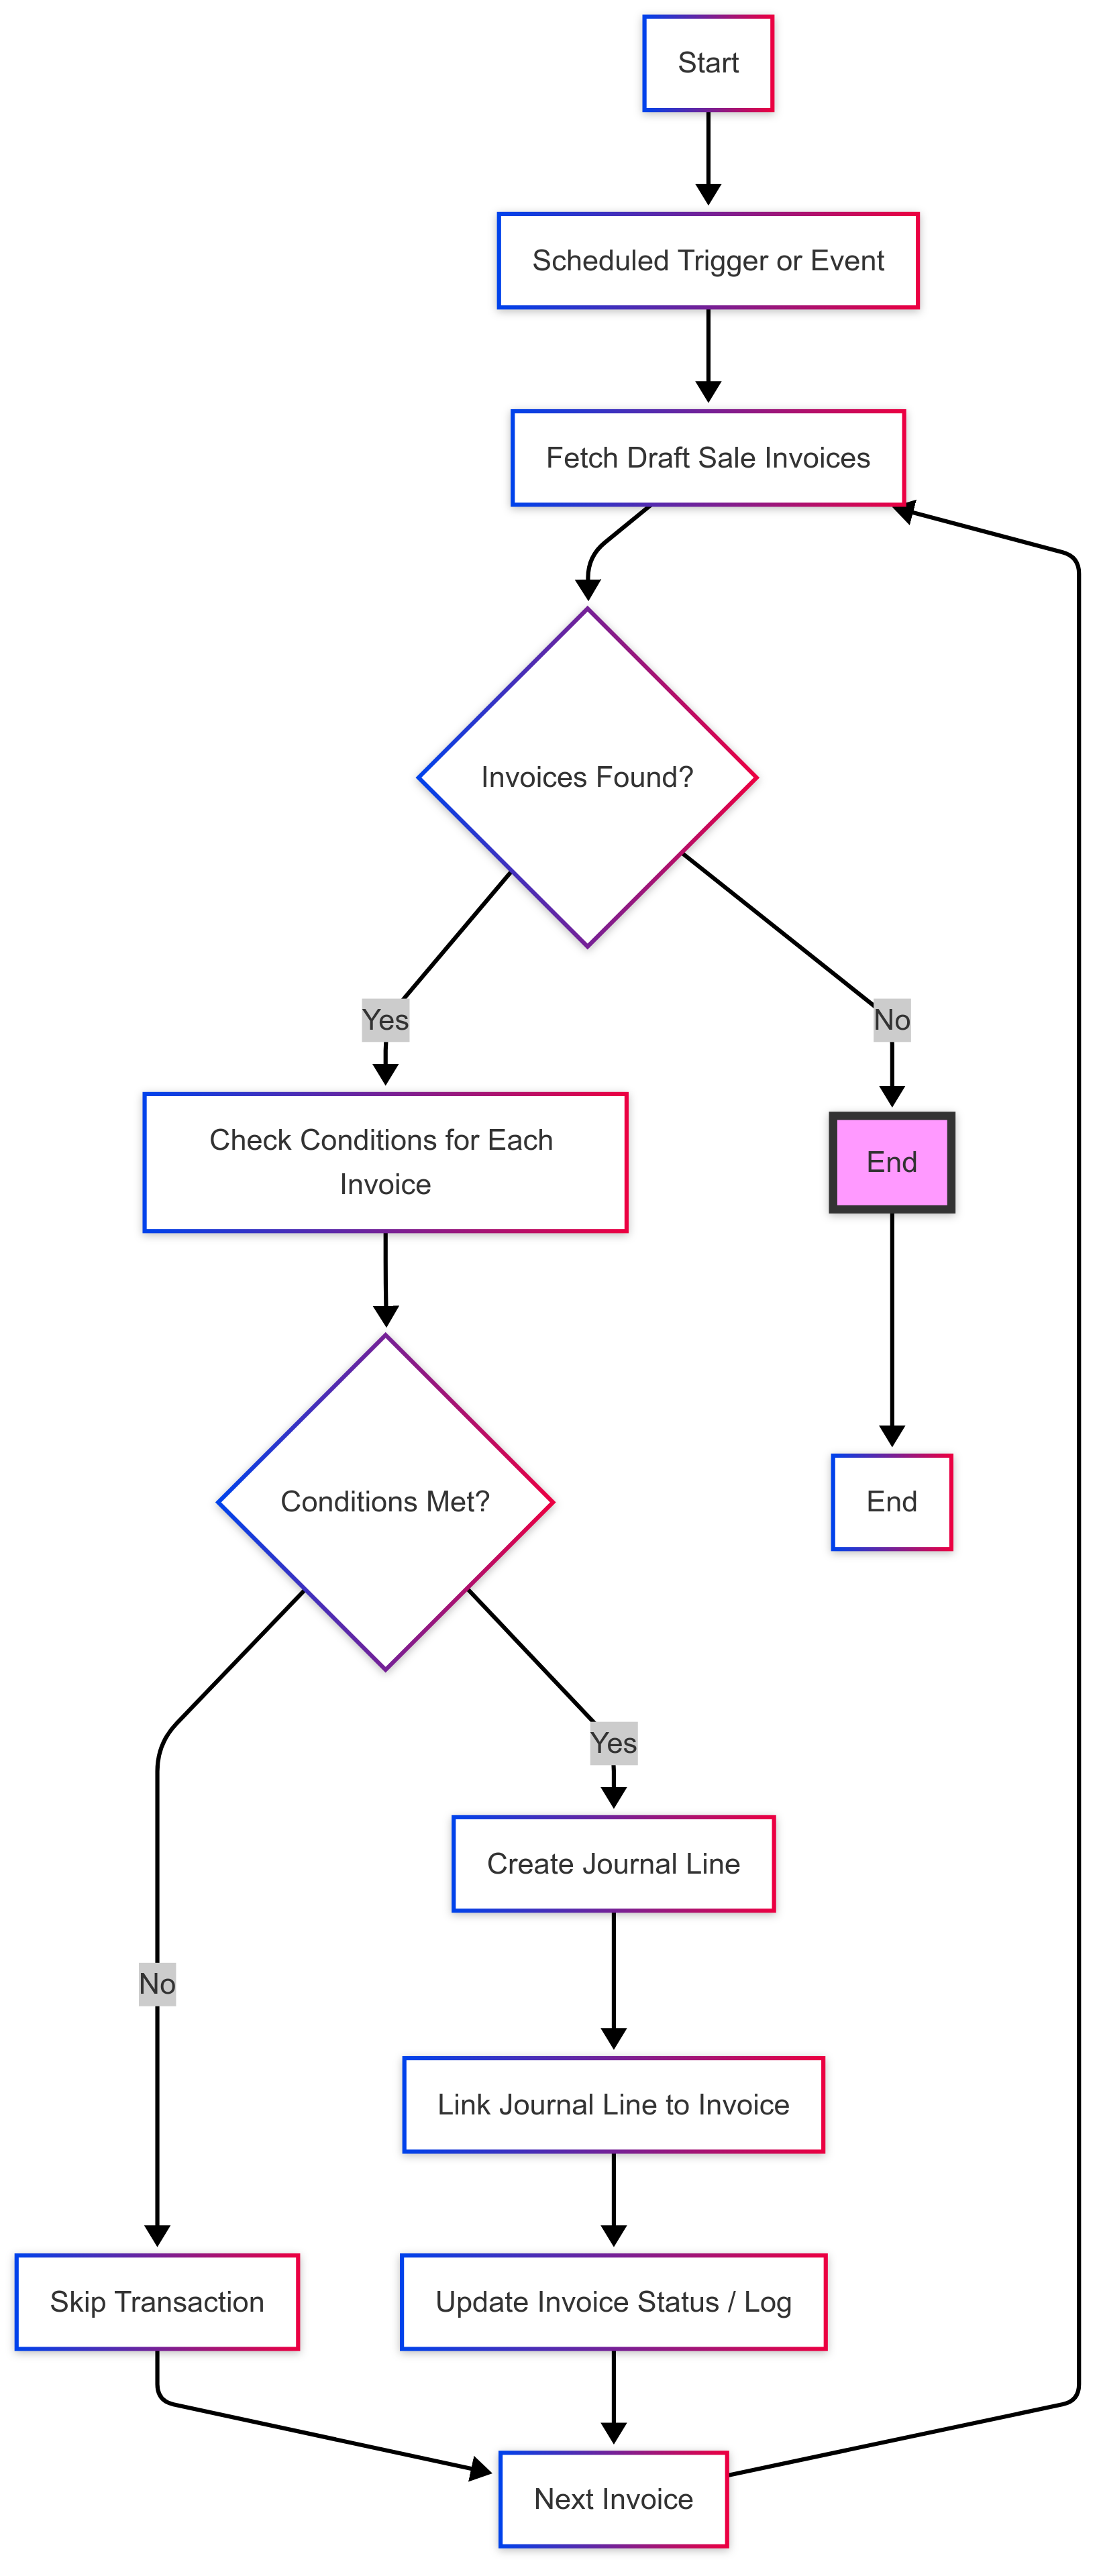
\includegraphics[width=\linewidth]{diagram/autoposting.png}
\end{minipage}

\noindent\textbf{Custom Logic to Calculate Payment Terms}

\noindent\textbf{Purpose:} Use custom logic to determine due dates and payment amounts based on special payment terms. This proves useful when special payment schemes are present in 
business, such as offering a discount for early settlement or special payment arrangements.
\medskip

\noindent\textbf{Implementation Steps:}
\medskip

\begin{minipage}{0.5\textwidth}
\begin{enumerate}
    \item Extend the account.payment.term Model:
    The account.payment.term model, which governs 
    payment terms, will be updated to hold custom fields 
    that enable the storage of unique rules governing the 
    payment term, such as:
    
    \begin{enumerate}
        \item Discount rate
        \item Early payment discount
        \item Custom payment frequency or amounts
    \end{enumerate}
    
    \item Override the Compute Method:    
    The compute method of the account.payment.term 
    model is overridden to include custom logic in 
    computing due dates and payment amounts from the 
    unique rules defined in the new fields.
    
    \item Return Custom Payment Terms:
    The overridden method will give a list of tuples 
    consisting of a due date and the amount due for each 
    period.

\end{enumerate}

\end{minipage}%
\hfill
\begin{minipage}{0.45\textwidth}
    \centering
    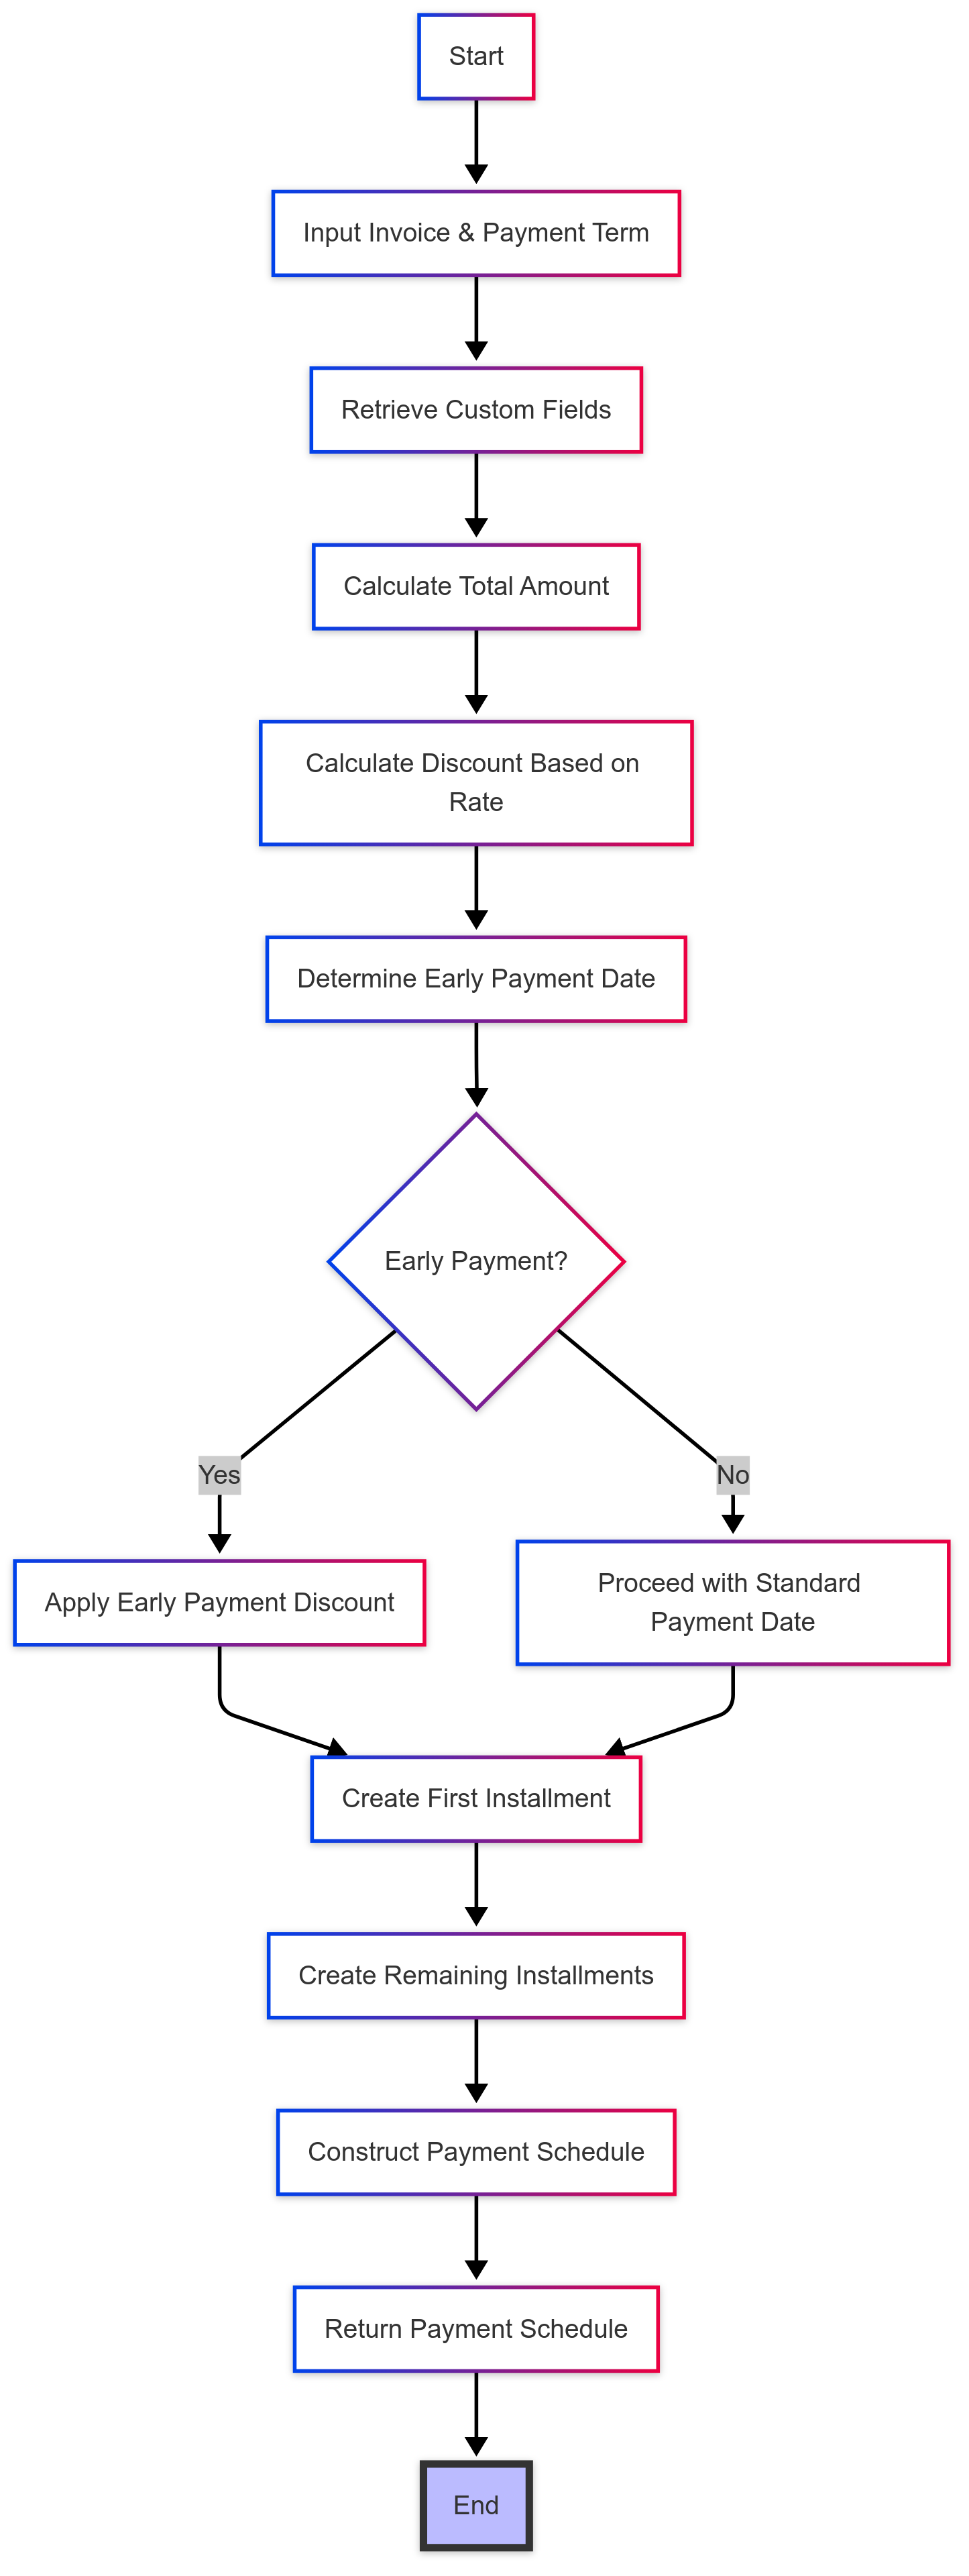
\includegraphics[width=\linewidth]{diagram/paymenttermcustomization.png} 
\end{minipage}

\subsubsection{Customization of Views and Actions}
Odoo's highly modular architecture allows for extensive 
customization of views and actions to 
enhance usability and adapt to specific business 
requirements. This chapter presents two 
practical illustrations of view customization in the 
Accounting module: enhancing invoice forms 
and designing tailored list views of aged receivables.

\begin{enumerate}
    \item Enhancing Invoice Views by Adding Custom Fields
    \textbf{Objective:} 

    To improve invoice forms to display additional information such as 
    custom business fields or related model data, improving data visibility 
    and productivity.
    \medskip

\begin{minipage}{0.5\textwidth}
    \textbf{Implementation Steps:}
    \begin{enumerate}
        \item Identify the Target View: Recognize the view to be customized 
        (e.g., account.move form view for invoices).
        \item Inherit the View: Use XML to inherit the base view by using the inherit\_id tag. This avoids overwriting base views and maintains upgrade compatibility.
        \item Add Custom Fields: Insert new fields from existing fields in the account.move model or add new fields (e.g., x\_branch\_id, x\_customer\_ref).
        \item Place Fields Strategically: Use Odoo's XML positioning attributes (before, after, inside) to place new fields in a convenient position.
    \end{enumerate}
\end{minipage}%
\hfill
\begin{minipage}{0.45\textwidth}
    \centering
    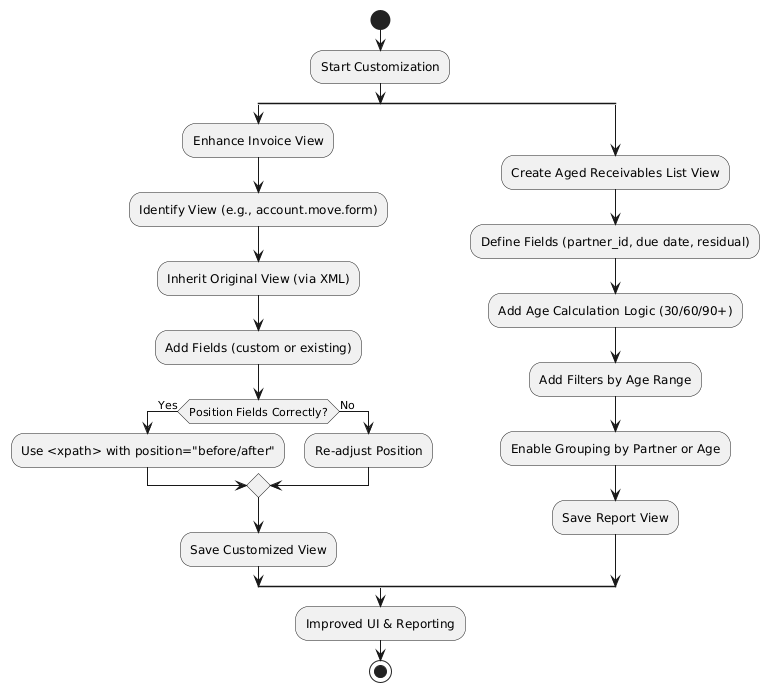
\includegraphics[width=\linewidth]{diagram/Customization_of_views&action.png}
\end{minipage} 
    \medskip

    \textbf{Result:}

    Users can see additional invoice details without having to navigate away from the page, supporting enhanced decision-making and efficient workflow.

    \item Custom List Views for Aged Receivables
    
    \textbf{Objective:}

    To provide a list view that presents overdue customer invoices segmented by age, to facilitate quicker collection follow-up and cash flow visibility.
    \medskip

    \textbf{Implementation Steps:}
    \begin{enumerate}
        \item Create a New List View: Specify a new list view (tree type) for the account.move model, filtered on customer invoices.
        \item Add Key Fields:
        \begin{enumerate}
            \item partner\_id: Customer name
            \item invoice\_date\_due: Payment due date
            \item residual: Outstanding amount
            \item age: A computed field reflecting how overdue the invoice is (e.g., 0–30, 31–60, 61–90, 90+ days)
        \end{enumerate}
        \item Add Domain Filters:
        
        Support filtering by invoice age buckets with filter elements in XML or custom search screens.
        \item Support Grouping:
        
        Support grouping by customer (partner\_id) or age buckets to quickly analyze customer debt composition.
    \end{enumerate}

    \textbf{Result:}

    Accounting users are provided with a tailored UI to monitor past-due receivables, prioritize collections, and export structured data for reporting.

\end{enumerate}

\subsubsection{Reporting Customization}
Odoo has a very flexible reporting engine that may be customized to generate specialized financial reports to serve specific business requirements. The customizations may either be done over standard financial reports or completely customized report templates.

\begin{enumerate}
    \item \textbf{Changing Standard Profit \& Loss and Balance Sheet Reports}
    \textbf{Purpose:}

    To alter the organization, content, and logic of generic financial reports (e.g., the Profit \& Loss or Balance Sheet) to suit business-specific metrics and classifications.
    \medskip

    \textbf{Implementation Steps:}
    \begin{enumerate}
        \item Find the Report to Change: Identify the target report, for instance:
        \begin{enumerate}
            \item account.account\_financial\_report\_profitandloss
            \item account.account\_financial\_report\_balancesheet
        \end{enumerate}
        \item Inherit the Report Template: Create a custom report by inheriting the underlying financial report XML or Python code.
        \item Change Report Lines:
        \begin{enumerate}
            \item Add new report lines to show additional financial information.
            \item Adjust existing lines to alter calculations, formulas, or display settings.
            \item Remove unnecessary lines that do not apply to the company reporting needs.
        \end{enumerate}
        \item Change Report Options: Modify filters such as:
        \begin{enumerate}
            \item Date ranges
            \item Comparison periods (e.g., year-over-year, month-over-month comparisons)
            \item Analytic filters on projects, departments, or cost centers
        \end{enumerate}
    \end{enumerate}
    \medskip

    \newpage
    \item \textbf{Creating Custom QWeb or Excel Reports}
    
    \begin{minipage}{0.45\textwidth}
        \begin{enumerate}
            \item QWeb-Based Reports
            
            \textbf{Purpose:} 
            
            To produce custom PDF reports with branded and properly formatted output through Odoo's templating engine.
            \medskip

            \textbf{Implementation Steps:}
            \begin{enumerate}
                \item Create a new QWeb template by XML.
                \item Use Odoo ORM within a matching Python report class in order to pull necessary financial data.
                \item Display and format the data through QWeb syntax (loops, conditions, formatting).
                \item Bind the report to an action to enable users to create using the UI.
            \end{enumerate}
            \item Excel-Based Reports (XLSX)
            
            \textbf{Purpose:} 
            
            Create spreadsheet reports, which may further be edited by users, exchanged, or uploaded into third-party systems.
            \medskip

        \end{enumerate}
    \end{minipage}
    \hfill
    \begin{minipage}{0.4\textwidth}
        \centering
        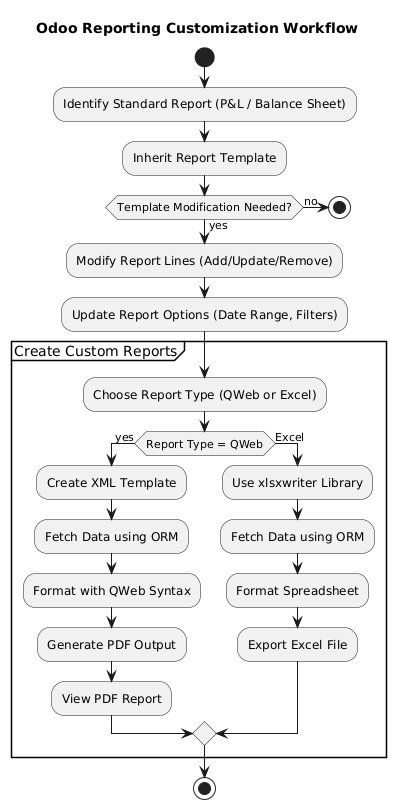
\includegraphics[width=\linewidth]{diagram/reporting_customization_workflow.png}
    \end{minipage}

    \textbf{Implementation Steps:}
        \begin{enumerate}
            \item Make use of the xlsxwriter Python library for generating a dynamic Excel document.
            \item Retrieve needed fiscal records via Odoo ORM practices (e.g., journal entry, balances).
            \item Render headers, insert formulas, and insert rows of data by utilizing functions through xlsxwriter.
            \item Give the developed Excel file as a downloadable attachment or in a report that is scheduled.
        \end{enumerate}
\end{enumerate}

\subsection{C4 Model - Component Diagram (C3 - Accounting Internals)}
\begin{center}
    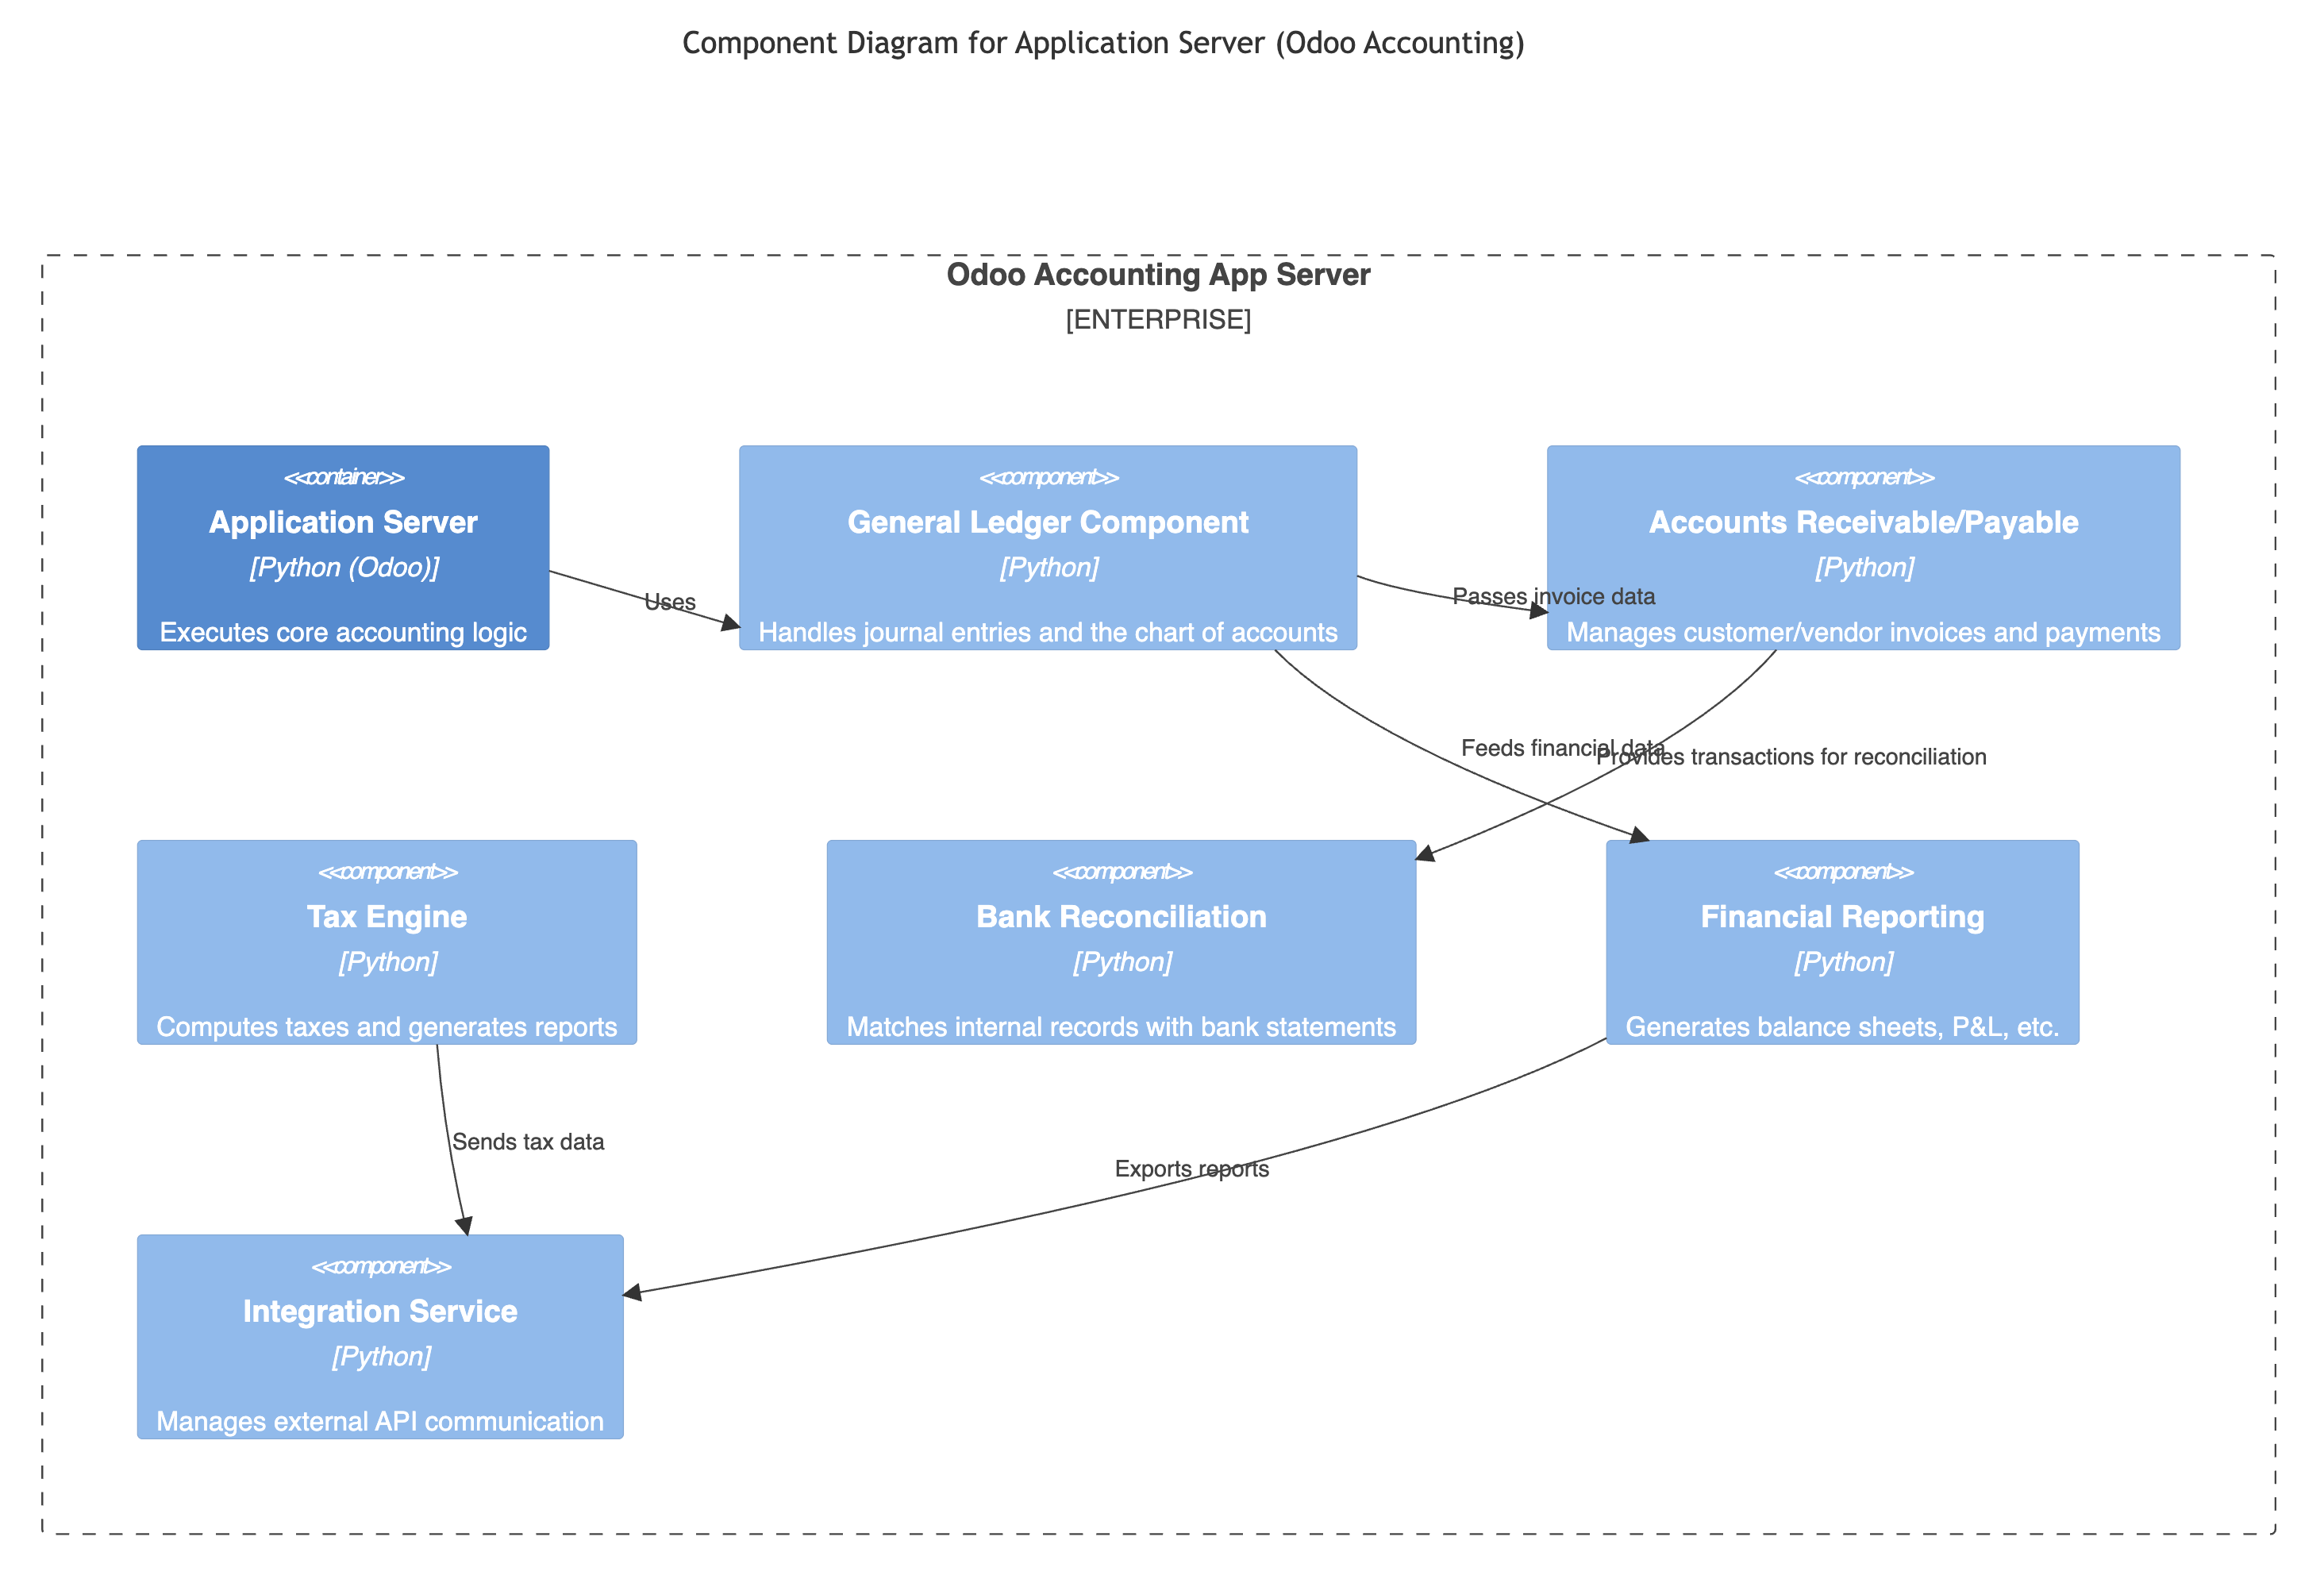
\includegraphics[width=0.8\linewidth]{diagram/C3.png}
\end{center}

\noindent This component diagram provides a high-level description of the Odoo Accounting Module, breaking it down into its primary functional components and how they interact with each other. Each component embodies a specific set of duties that collectively enable end-to-end financial management within the system.

\begin{enumerate}
    \item \textbf{Invoice Management}
    
    \textbf{Description:} Manages the creation, modification, and life cycle of customer and vendor invoices.
    \medskip

    \textbf{Key Responsibilities:}
    \begin{enumerate}
        \item Create, update, and delete invoice records.
        \item Create and export invoice documents (PDFs).
        \item Control invoice statuses (e.g., Draft, Posted, Paid, Cancelled).
    \end{enumerate}

    \textbf{Interfaces:}
    \begin{enumerate}
        \item Create and fetch invoice data.
        \item Update invoice state and related fields.
    \end{enumerate}

    \textbf{Dependencies:}
    \begin{enumerate}
        \item Tax Engine – for calculation of tax in real-time.
        \item Payment Handling – for linking payments and for updation of invoice payment status.
    \end{enumerate}

    \item \textbf{Payment Handling}
    
    \textbf{Description:} Responsible for handling the processing and recording of payments that come in and go out.
    \medskip

    \textbf{Key Responsibilities:}
    \begin{enumerate}
        \item Record customer payments and vendor disbursements.
        \item Link payments with related invoices or bills.
        \item Generate payment receipts and reconcile books of accounts.
    \end{enumerate}

    \textbf{Interfaces:}
    \begin{enumerate}
        \item Register and read payment information.
        \item Associate payments with accounting documents.
    \end{enumerate}

    \textbf{Dependencies:}
    \begin{enumerate}
        \item Invoice Management – to account for payments.
        \item Reconciliation Engine – to reconcile payments with bank accounts.
    \end{enumerate}

    \item \textbf{Reconciliation Engine}
        
    \textbf{Description:} Reconciles bank statement line with internal accounting postings.
    \medskip

    \textbf{Key Responsibilities:}
    \begin{enumerate}
        \item Import and interpret bank statements.
        \item Automatically match transactions according to configurable rules.
        \item Offer manual and auto-recommended reconciliations.
    \end{enumerate}

    \textbf{Interfaces:}
    \begin{enumerate}
        \item Import bank information and define reconciliation logic.
        \item Review and approve reconciliations.
    \end{enumerate}

    \textbf{Dependencies:}
    \begin{enumerate}
        \item Payment Handling – to read payment records.
        \item Reporting \& Analytics – to enable reconciliation reporting and auditing.
    \end{enumerate}

    \item \textbf{Reporting \& Analytics}
            
    \textbf{Description:} Generates financial and analytical reports to external and internal stakeholders.
    \medskip

    \textbf{Key Responsibilities:}
    \begin{enumerate}
        \item Prepare primary financial statements (e.g., P\&L, Balance Sheet).
        \item Provide dynamic dashboards and drill-down.
        \item Generate customized financial reports.
    \end{enumerate}

    \textbf{Interfaces:}
    \begin{enumerate}
        \item Configure report parameters and layouts.
        \item Export data to PDF, Excel, or web views.
    \end{enumerate}

    \textbf{Dependencies:}
    \begin{enumerate}
        \item Dependent on all other components for data aggregation and metrics.
    \end{enumerate}

    \item \textbf{Tax Engine}
                
    \textbf{Description:} Verifies compliance with local tax legislation and calculates taxes.
    \medskip

    \textbf{Key Responsibilities:}
    \begin{enumerate}
        \item Calculate recoverable taxes upon invoice or bill processing.
        \item Schedule tax codes, tax rates, and fiscal postings.
        \item Prepare statutory tax reports.
    \end{enumerate}

    \textbf{Interfaces:}
    \begin{enumerate}
        \item Develop and implement tax regulations.
        \item Generate reports (e.g., VAT, GST summaries).
    \end{enumerate}

    \textbf{Dependencies:}
    \begin{enumerate}
        \item Invoice Management – in aid of calculation of tax on transactions.
    \end{enumerate}

\end{enumerate}

\subsection{C4 Model - Code Diagram (C4 - Illustrative Examples)}
\begin{center}
    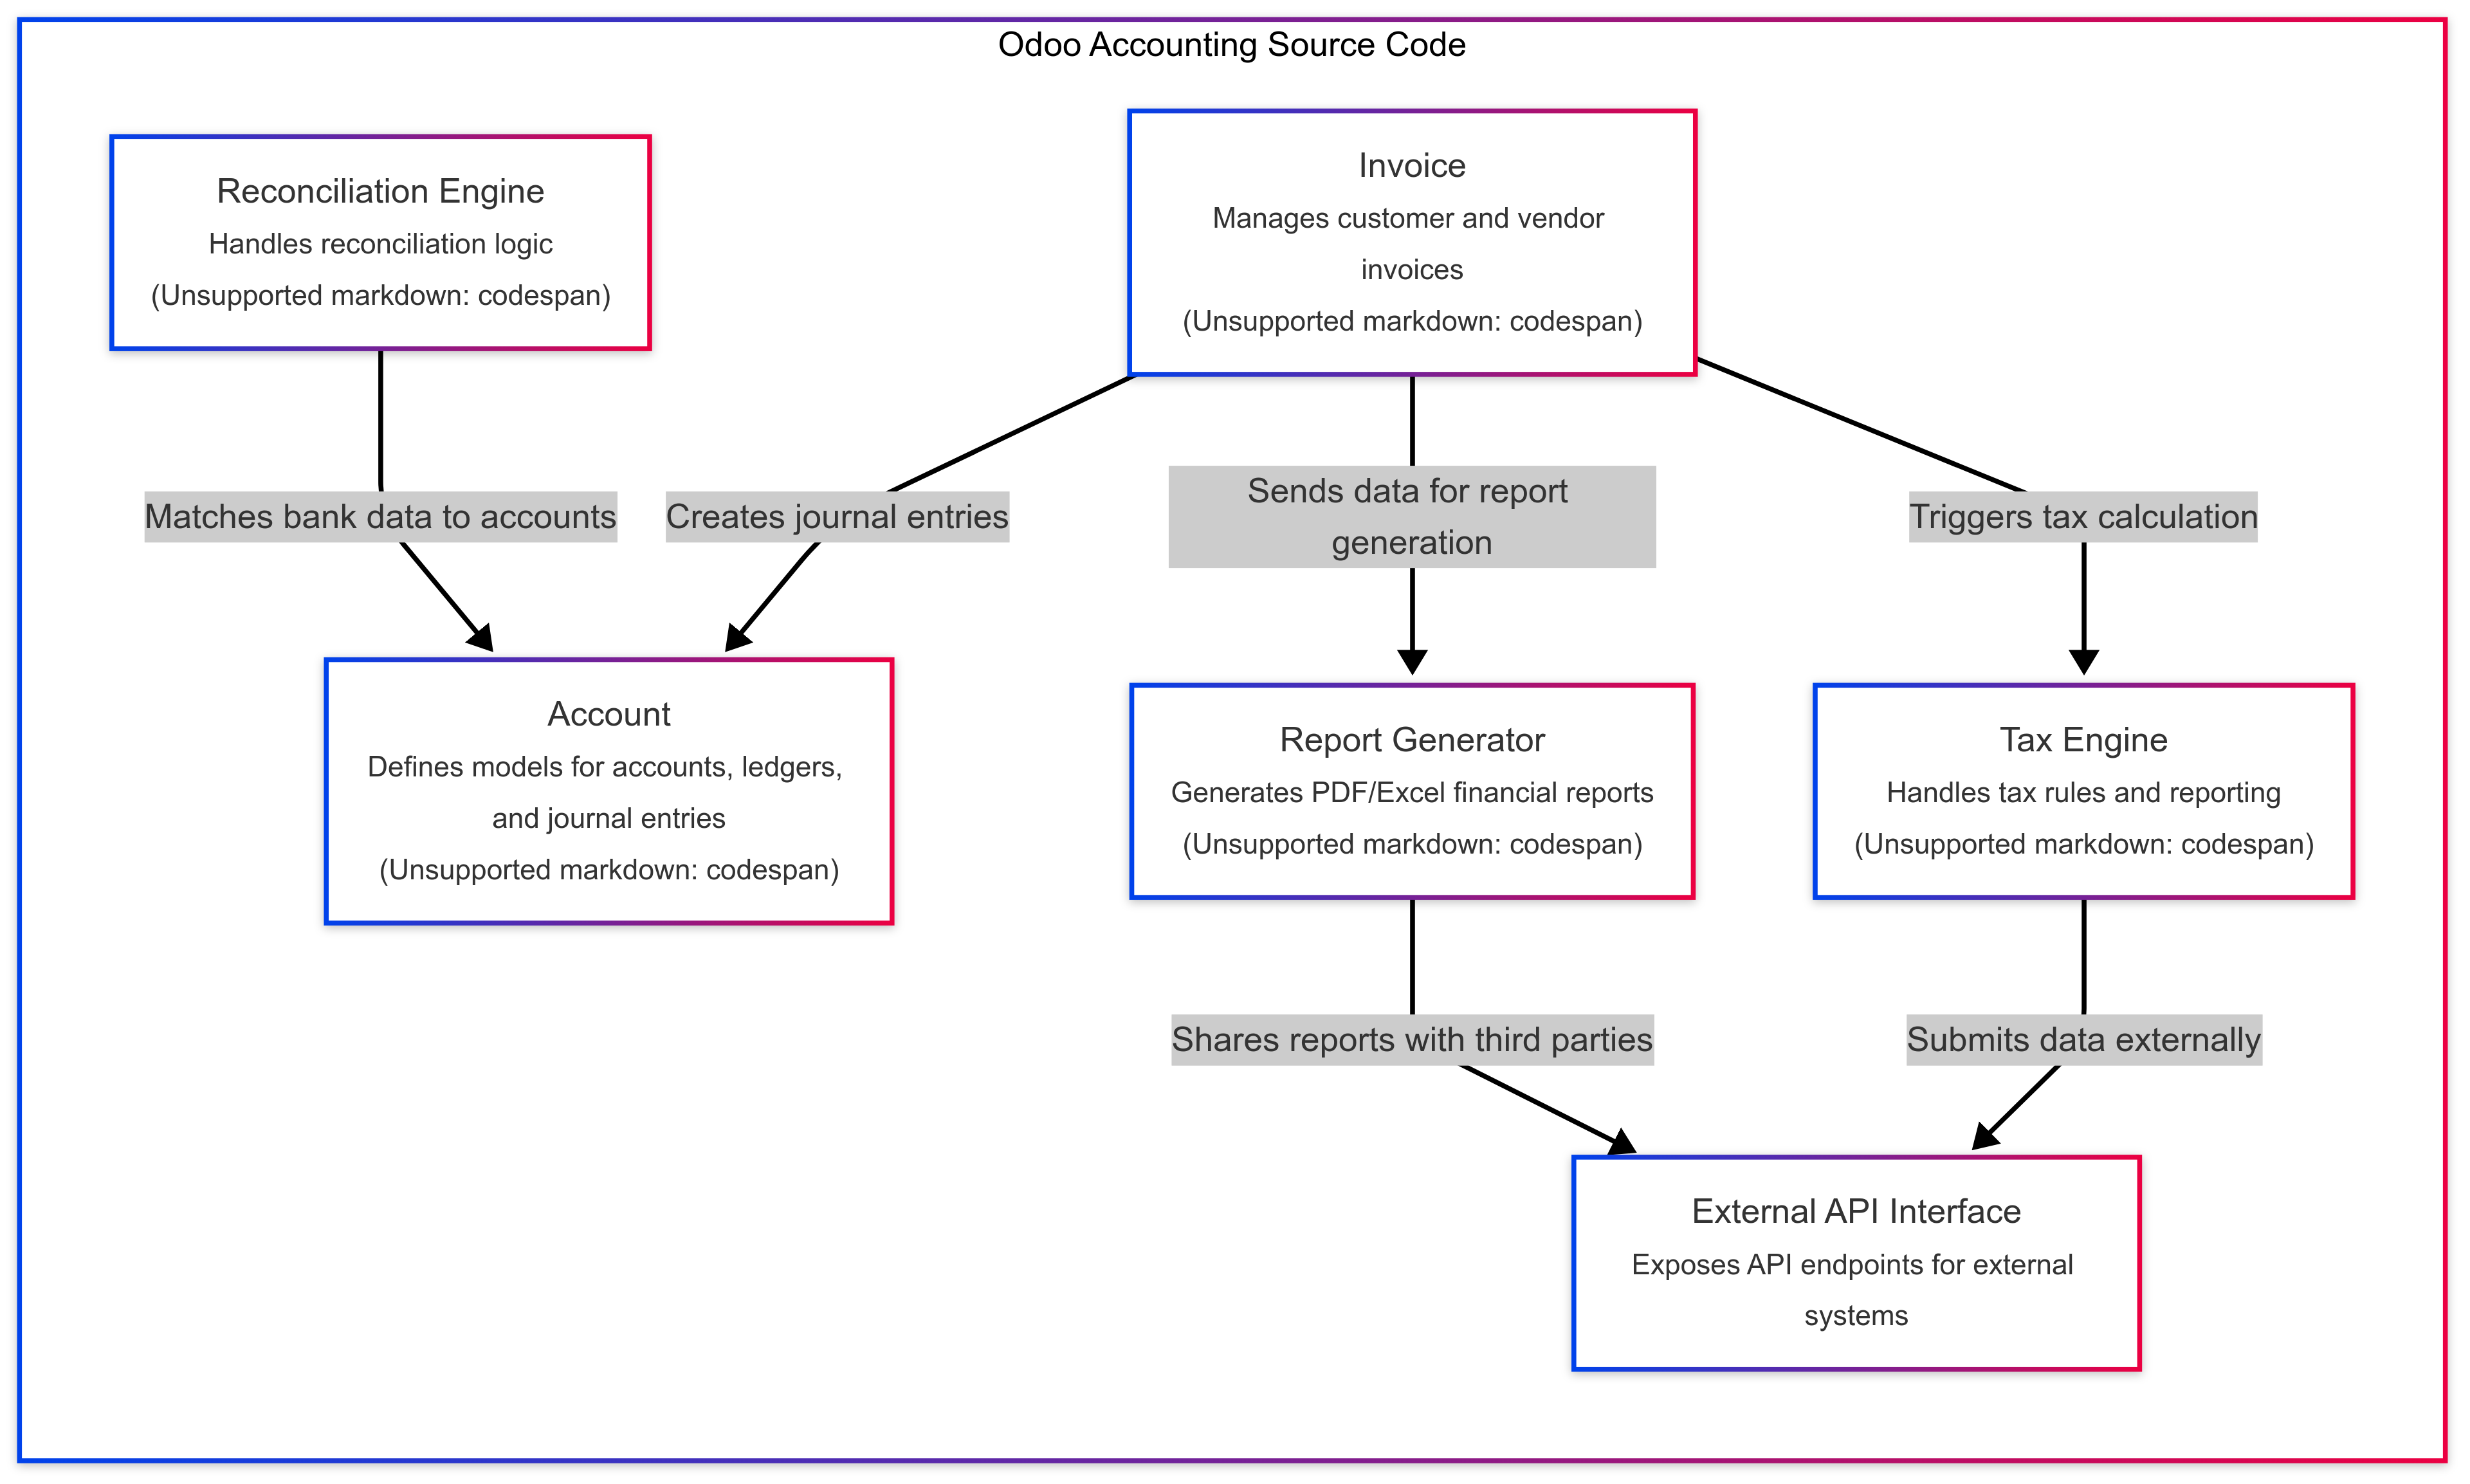
\includegraphics[width=0.8\linewidth]{diagram/C4_model.png}
\end{center}

\noindent This diagram illustrates the core components of the Odoo Accounting source code and their interactions. The Invoice component manages customer and vendor invoices, creating journal entries in the Account module, which defines models for accounts, ledgers, and journal entries. The Reconciliation Engine handles matching bank data to existing account records to ensure 
accurate financial reconciliation. The Report Generator component is responsible for producing financial reports in PDF or Excel formats and shares these reports with third parties. The Tax Engine manages tax calculations and rules, triggering tax computations during invoice 
processing and submitting relevant tax data externally. All report sharing and tax submission 
activities interact with the External API Interface, which exposes API endpoints to enable 
third-party systems to access reports and tax-related data. Overall, these components work 
together to facilitate robust, automated accounting processes within Odoo.

\newpage
\section{Deployment}
\subsection{Deployment Considerations}
Implementation of the Odoo Accounting module requires careful planning and strategic 
deployment to prevent a disruption, comply with finance standards, and smooth adoption by 
users. Some key areas to explore are outlined below:

\begin{center}
    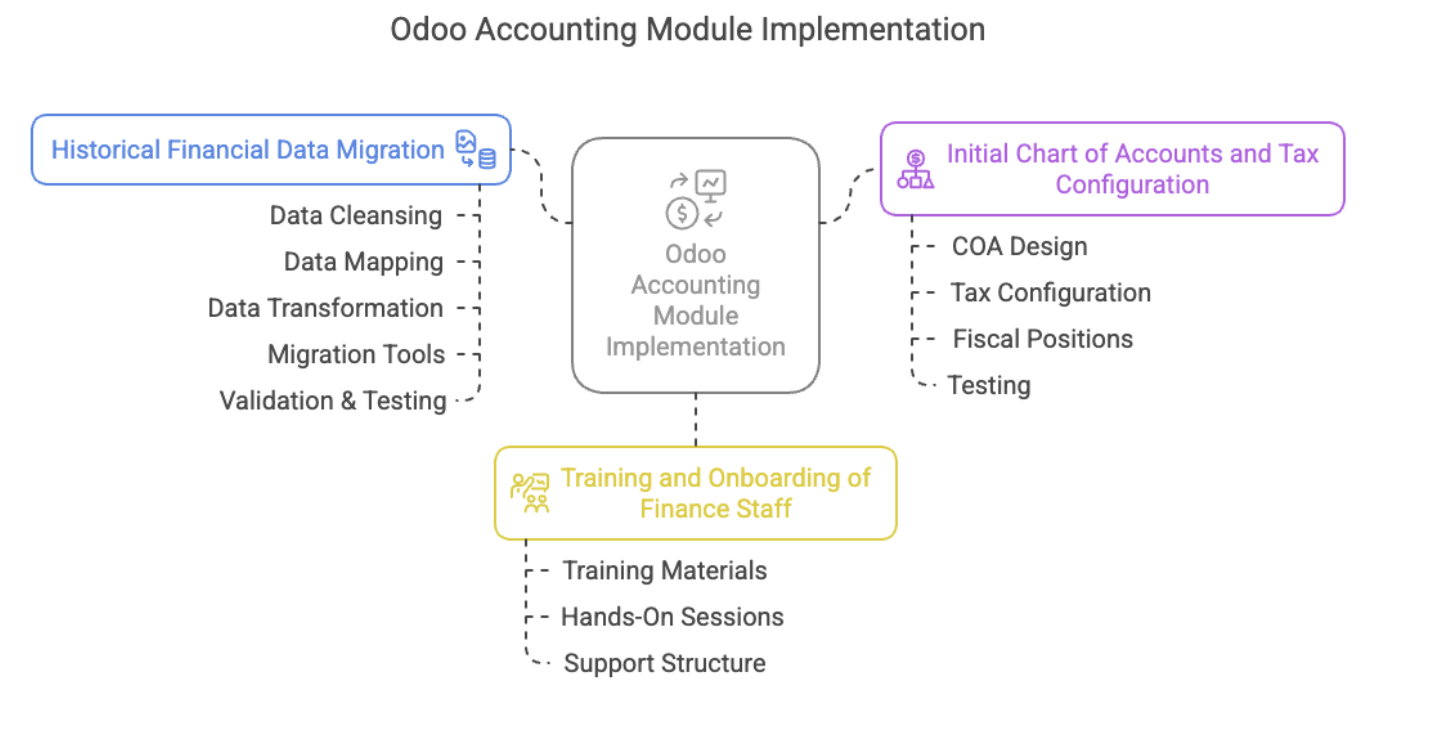
\includegraphics[width=0.8\linewidth]{diagram/odoo_accounting_module_implementation.png}
\end{center}

\begin{enumerate}
    \item \textbf{Historical Financial Data Migration}

    \textbf{Goal:} Ensure continuity of financial reporting and an auditable complete financial history in Odoo.
    \medskip

    \textbf{Key Considerations:}
    \begin{enumerate}
        \item Data Cleansing: Clean and verify current legacy financial records for the elimination of duplicates, errors, or inconsistencies.
        \item  Data Mapping: Map your existing data fields onto Odoo's data model (e.g., accounts, partners, transactions).
        \item Data Transformation: Convert legacy forms into Odoo-compatible formats.
        \item Migration Tools: Use Odoo's native import features or third-party tools (e.g., ETL tools or scripts).
        \item Validation \& Testing: Verify the integrity and accuracy of imported data through extensive reconciliation and test cases.
    \end{enumerate}
    \medskip

    \textbf{Best Practices:}
    \begin{enumerate}
        \item Run a pilot migration using a small data set.
        \item  Involve finance personnel early on for validation and feedback.
        \item Data Transformation: Convert legacy forms into Odoo-compatible formats.
        \item Document the entire process for transparency and future audits.
    \end{enumerate}

    \item \textbf{Initial Chart of Accounts (COA) and Tax Configuration}

    \textbf{Goal:} Establish a solid financial foundation that is compliant, reduces reporting, and supports business-specific workflows.
    \medskip

    \textbf{Key Considerations:}
    \begin{enumerate}
        \item COA Design: Create a rational and scalable chart of accounts based on accounting standards and reporting needs.
        \item Tax Configuration: Set up all relevant taxes, like sales tax, VAT, GST, etc., with the correct percentages and rules of usage.
        \item Fiscal Positions: Set up fiscal positions to handle regional tax variations by customer/vendor locations or exemptions.
        \item Testing: Test common transactions (e.g., invoices, vendor bills) to check tax calculations and account mappings.
    \end{enumerate}
    \medskip

    \textbf{Best Practices:}
    \begin{enumerate}
        \item Use a standard COA template as a base and then adapt it to your business.
        \item Test configurations with a certified accountant.
        \item Document your COA design and tax logic for regulatory purposes.
    \end{enumerate}
    \medskip

    \item \textbf{Training and Onboarding of Finance Staff}

    \textbf{Goal:} Get the finance team ready to learn and utilize the Odoo Accounting module efficiently.
    \medskip

    \textbf{Key Considerations:}
    \begin{enumerate}
        \item Training Materials: Provide step-by-step guides, quick reference materials, and video tutorials that are workflow-specific.
        \item Hands-On Sessions: Offer hands-on training in real-life scenarios to support learning.
        \item Support Structure: Set up support structures for maintenance support (e.g., internal helpdesk, FAQs, power users).
    \end{enumerate}
    \medskip

    \textbf{Best Practices:}
    \begin{enumerate}
        \item Start with fundamental concepts and build up to advanced features (e.g., reconciliation rules, financial reports).
        \item Offer training in multiple formats (live sessions, recorded webinars, interactive documentation).
        \item Encourage open communication and feedback to continually improve the onboarding experience.
    \end{enumerate}
    
\end{enumerate}

\newpage
\section{Maintenance}
\subsection{Maintenance and Updates}
Routine upkeep and updates of the Odoo Accounting module are necessary to ensure proper 
functionality, security, regulatory compliance, and responding to evolving business requirements. 
Below are some of the key areas that should be addressed:
\medskip
\begin{enumerate}
    \item \textbf{COA upgrade}
    
\begin{minipage}{0.45\textwidth}
    \textbf{Purpose:} To support restructurings within the organization, future expansion, or to meet updated accounting standards.

    \medskip
    \textbf{Key Considerations:}
    \begin{enumerate}
        \item Strategic Planning: Plan for how the COA updates will affect historical data, reporting, and integrations.
        \item Mapping Old to New COA: Create a clean mapping of the old accounts to the new structure to ensure consistency.
        \item Data Migration: Utilize data migration scripts or tools to realign the historical entries with the new COA.
        \item Testing \& Validation: Perform extensive tests to ensure reports, journal entries, and account balances are correct.
    \end{enumerate}
\end{minipage}%
\hfill
\begin{minipage}{0.45\textwidth}
    \centering
    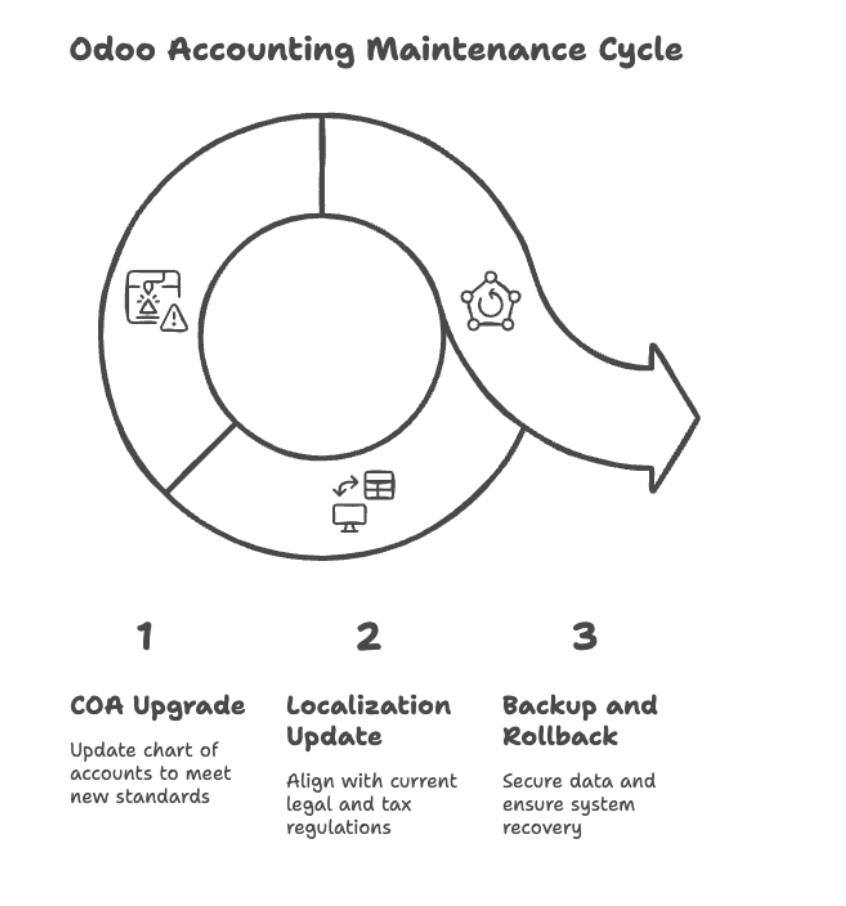
\includegraphics[width=\linewidth]{diagram/odoo_accounting_maintenance_cycle.png}
\end{minipage}

\medskip
\textbf{Best Practices:}
\begin{enumerate}
    \item Upgrade first in a staging/test environment.
    \item Engage your accounting team during the upgrade process for review and validation.
    \item Maintain complete records of all updates, including before-and-after mapping and impact 
	analysis.
\end{enumerate}

    \item \textbf{Localization and Compliance Update Management}

    \textbf{Purpose:} Having the system aligned with most recent legal, tax, and financial regulations of each operating country.

    \textbf{Key Considerations:}
    \begin{enumerate}
        \item Regulatory Monitoring: Monitor changes in national or international accounting regulations (e.g., VAT changes, reporting obligations) constantly.
        \item Applying Localization Updates: Install Odoo localization modules and patches relevant to your country from time to time (e.g., electronic invoice, SAF-T, GST).
        \item Testing Post-Updates: Validate the installed updates are functional and do not interfere with running workflows or reporting.
    \end{enumerate}

    \textbf{Best Practices:}
    \begin{enumerate}
        \item Subscribe to Odoo enterprise updates or certified localization partners.
        \item Utilize a local certified accountant to validate all compliance updates.
        \item Log each compliance update and its effect on reporting, taxation, and workflow.
    \end{enumerate}
    
    \item \textbf{Backup and Rollback Strategies}
    
    \begin{minipage}{0.45\textwidth}
    \textbf{Purpose:} To safeguard critical financial data and system recovery in case of failures, data loss, or corruption.
    
    \medskip
    \textbf{Key Considerations:}
    \begin{enumerate}
        \item Backup Schedule: Have a regular schedule (e.g., every day, weekly) based on volume and urgency of transactions.
        \item Secure Storage Location: Store backups securely and redundantly (e.g.,encrypted cloud, offsite servers).
        \item Rollback Process: Set up and follow explicit rollback processes to restore backups when something goes wrong during emergencies or after failed updates.
        \item Backup Verification: Periodically test the backup restoration process to guarantee the integrity of the backup and rollback.
    \end{enumerate}

    \textbf{Best Practices:}
    \begin{enumerate}
        \item Make backup procedures automated with scripts or Odoo-compatible utilities.
        \item Include versioning and snapshot backups for quick recovery alternatives.
        \item Have at least one offsite backup and detail the entire disaster recovery process.
    \end{enumerate}
    \end{minipage}%
    \hfill
    \begin{minipage}{0.45\textwidth}
        \centering
        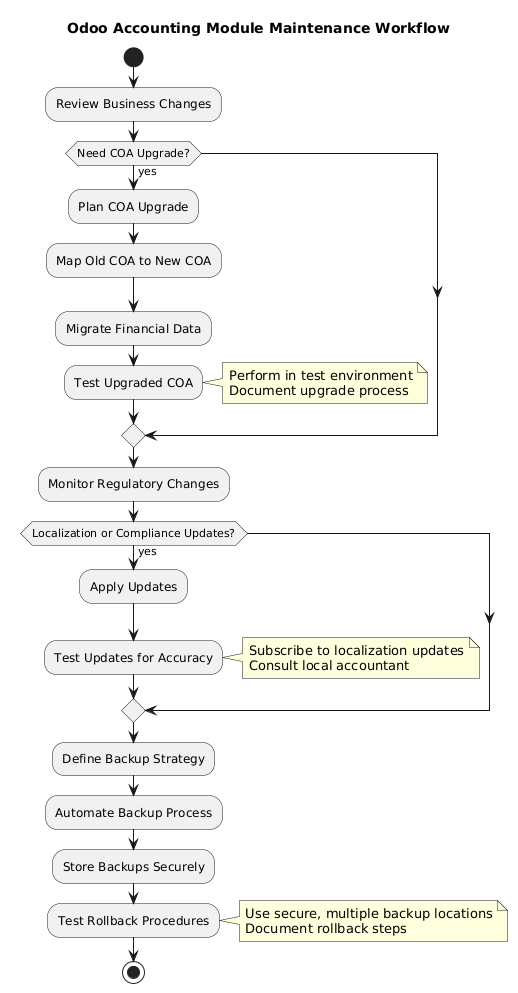
\includegraphics[width=\linewidth]{diagram/accounting_maintenance_workflow.png}
    \end{minipage}
\end{enumerate}

\newpage
\section{Appendices}
\subsection{Glossary of Terms}

\begin{longtable}{|l|p{10cm}|}
    \hline
    \textbf{Term} & \textbf{Definition} \\
    \hline
    \texttt{Account} & A record in the general ledger that is used to sort and store financial transactions (e.g., Cash, Sales, Expense). \\
    \hline
    \texttt{Chart of Accounts (COA)} & A structured list of all the accounts used by an organization to classify and record financial transactions. \\
    \hline
    \texttt{Fiscal Position} & A configuration in Odoo that determines which taxes and accounts are applied based on a customer's or vendor's country, company type, or location. \\
    \hline
    \texttt{Journal Entry (Move)} & A complete record of a financial transaction in the general ledger. In Odoo, this is called a "Move." \\
    \hline
    \texttt{Move Line} & An individual line within a journal entry that represents a debit or credit to an account. \\
    \hline
    \texttt{Journal} & A record that groups financial entries of a specific type (e.g., Sales Journal, Purchase Journal, Bank Journal). \\
    \hline
    \texttt{Reconciliation} & The process of matching and validating transactions in the bank statement against the accounting entries. \\
    \hline
    \texttt{Analytic Account} & A secondary axis of financial analysis used to group transactions for projects, departments, or cost centers. \\
    \hline
    \texttt{Partner} & A contact record in Odoo, which can be a customer, vendor, or both. \\
    \hline
    \texttt{Invoice} & A commercial document issued by a seller to a buyer indicating the products, quantities, and agreed prices. \\
    \hline
    \texttt{Bill} & An invoice received from a supplier, which records the company's payables. \\
    \hline
    \texttt{Credit Note} & A document issued to reduce the amount owed on a previously issued invoice. \\
    \hline
    \texttt{Debit Note} & A document used to increase the amount payable on a bill, often due to errors or additional charges. \\
    \hline
    \texttt{Payment Term} & A set of rules that determine how and when an invoice should be paid, including possible early-payment discounts. \\
    \hline
    \texttt{Tax} & A financial charge calculated on a transaction, managed through tax rules and tax groups in Odoo. \\
    \hline
    \texttt{Tax Report} & A summary of tax collected and paid, typically used for VAT or GST filing. \\
    \hline
    \texttt{Bank Statement} & A record of transactions from a bank account, which can be imported or manually created in Odoo. \\
    \hline
    \texttt{Asset} & A long-term resource owned by a company, managed through Odoo’s Asset Management for depreciation tracking. \\
    \hline
    \texttt{Deferred Revenue / Expense} & Revenues or expenses that are recognized in future periods and managed via deferral journals. \\
    \hline
    \texttt{Lock Date} & A date before which no changes can be made to accounting records, used to close financial periods. \\
    \hline
    \texttt{Audit Trail} & The log of changes and transactions recorded for traceability and compliance. \\
    \hline
    \texttt{Cash Basis Accounting} & An accounting method where revenues and expenses are recorded when cash is received or paid. \\
    \hline
    \texttt{Accrual Accounting} & An accounting method where transactions are recorded when they occur, regardless of cash movement. \\
    \hline
    \texttt{Multi-Currency} & The ability to handle transactions, journals, and reporting in different currencies. \\
    \hline
    \texttt{Opening Balance} & The amount of money in an account at the beginning of a new fiscal period. \\
    \hline
    \texttt{Closing Entry} & An entry made at the end of an accounting period to close temporary accounts (e.g., revenues, expenses). \\
    \hline
    \texttt{Budget} & A financial plan that estimates revenue and expenses for a future period, which can be tracked via Odoo’s budgeting feature. \\
    \hline
    \texttt{Consolidation} & The process of combining financial data from multiple companies/entities into one unified report. \\
    \hline
\end{longtable}

\subsection{Acronyms and Abbreviations}
\begin{longtable}{|l|p{13cm}|}
    \hline
    \textbf{Acronym} & \textbf{Definition} \\
    \hline
    \texttt{AP} & Accounts Payable – Money a business owes to suppliers. \\
    \hline
    \texttt{AR} & Accounts Receivable – Money owed to a business by customers. \\
    \hline
    \texttt{BS} & Balance Sheet – A financial statement showing assets, liabilities, and equity. \\
    \hline
    \texttt{COA} & Chart of Accounts – Structured list of accounts used to categorize financial transactions. \\
    \hline
    \texttt{CFO} & Chief Financial Officer – The senior executive responsible for managing the financial actions of a company. \\
    \hline
    \texttt{CPA} & Certified Public Accountant – A qualified accountant licensed by a governing body. \\
    \hline
    \texttt{CR} & Credit – An accounting entry that either increases a liability or equity account or decreases an asset or expense account. \\
    \hline
    \texttt{DB} & Debit – An accounting entry that increases an asset or expense account or decreases a liability or equity account. \\
    \hline
    \texttt{DFA} & Depreciation, Fixed Assets – Related to the depreciation and management of fixed assets. \\
    \hline
    \texttt{ERP} & Enterprise Resource Planning – Integrated software used to manage business processes. \\
    \hline
    \texttt{FY} & Fiscal Year – A one-year period used for financial reporting. \\
    \hline
    \texttt{GAAP} & Generally Accepted Accounting Principles – Standard framework of guidelines for financial accounting. \\
    \hline
    \texttt{GL} & General Ledger – The primary accounting record summarizing all transactions. \\
    \hline
    \texttt{IFRS} & International Financial Reporting Standards – Global accounting standards. \\
    \hline
    \texttt{INV} & Inventory – The goods and materials a business holds for sale. \\
    \hline
    \texttt{IS} & Income Statement – Also known as Profit \& Loss Statement. \\
    \hline
    \texttt{JE} & Journal Entry – A record of a transaction in the accounting books. \\
    \hline
    \texttt{KPI} & Key Performance Indicator – Metrics that evaluate the success of an activity. \\
    \hline
    \texttt{P\&L} & Profit and Loss Statement – A financial report summarizing revenues and expenses. \\
    \hline
    \texttt{POS} & Point of Sale – System where sales transactions are completed. \\
    \hline
    \texttt{ROI} & Return on Investment – A measure of profitability. \\
    \hline
    \texttt{TAX/VAT} & Value Added Tax – A consumption tax added to the sale of goods and services. \\
    \hline
    \texttt{UoM} & Unit of Measure – Measurement unit for quantities in transactions. \\
    \hline
    \texttt{WHT} & Withholding Tax – Tax deducted at source on payments like salaries or dividends. \\
    \hline
    \texttt{API} & TApplication Programming Interface – Interface for communication between applications. \\
    \hline
    \texttt{CSV} & Comma-Separated Values – Format used to import/export tabular data. \\
    \hline
    \texttt{DB} & Database – Structured collection of data. \\
    \hline
    \texttt{ORM} & Object-Relational Mapping – Converts database data to object-oriented code. \\
    \hline
    \texttt{QWeb} & Odoo’s templating engine for reports and web views. \\
    \hline
    \texttt{SAAS} & Software as a Service – Software delivery model via the internet. \\
    \hline
    \texttt{UI} & User Interface – Visual part of the application. \\
    \hline
    \texttt{UX} & User Experience – Overall user interaction quality. \\
    \hline
    \texttt{UML} & Unified Modeling Language – Visual modeling language for systems. \\
    \hline
    \texttt{OCA} & Odoo Community Association – Organization supporting Odoo open-source development. \\
    \hline
    \texttt{Odoo.sh} & Odoo’s managed hosting platform for deployment. \\
    \hline
\end{longtable}

\subsection{Sample UML Diagrams}
\begin{minipage}{0.45\textwidth}
    \centering
    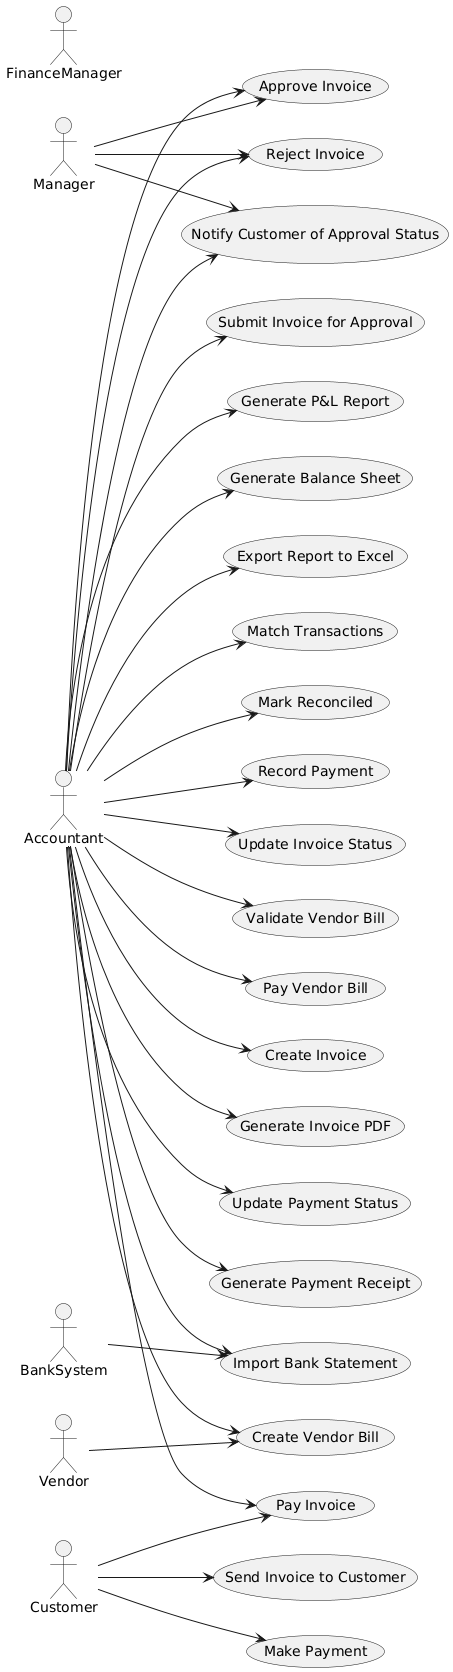
\includegraphics[width=\linewidth, height=0.8\textheight, keepaspectratio]{diagram/use_case_accounting.png}
\end{minipage}%
\hfill
\begin{minipage}{0.45\textwidth}
    \textbf{Use Case Diagram}
    This is a UML activity diagram illustrating the process flow with regard to handling invoices, payments, and communication with vendors in terms of different roles: 
    \medskip
    
    Finance Manager, Manager, Accountant, Bank System, Vendor, and Customer.
    \medskip

    \textbf{Roles and Activities:}

    \textbf{Finance Manager:}
    Approve or decline invoice.

	-Approve Invoice

	-Reject Invoice
    \medskip

    \textbf{Manager:} Inform customer of approval status, request approval of invoice.

    -Inform Customer of Approval Status	

	-Request Approval of Invoice
    \medskip

    \textbf{Accountant:} Performs multiple tasks with regard to handling invoices, financial reports, and payments.

    -Generate P\&L Report

	-Generate Balance Sheet

	-Export Report to Excel

	-Match Transactions

	-Mark Reconciled

	-Record Payment

	-Update Invoice Status

	-Validate Vendor Bill

	-Pay Vendor Bill

	-Create Invoice

	-Generate Invoice PDF

	-Update Payment Status

	-Generate Payment Receipt

	-Send Invoice to Customer
    \medskip

    \textbf{Bank System:} Handles bank statements and vendor bill payments.
    -Import Bank Statement

	-Create Vendor Bill

	-Pay Invoice
    \medskip

    \textbf{Vendor:} Prepares vendor bills and pays invoices.

	-Create Vendor Bill

	-Pay Invoice
    \medskip

    \textbf{Customer:} Receives invoices and makes payments.

    -Send Invoice to Customer

	-Make Payment
    \medskip

\end{minipage}

    \noindent\textbf{Key Flow:}
    \begin{itemize}
        \item The invoice is approved or rejected by the Finance Manager.
        \item The Manager initiates customer notification about approval status and sends the invoice for approval.
        \item The Accountant handles several finance document generation, transaction matching, payment recording, and invoice create/update tasks.
        \item Bank System allows importing bank statements, vendor bill generation, and invoice payment.
        \item Vendors issue bills and settle invoices.
        \item Customers receive bills and pay.
    \end{itemize}

    \noindent Generally, this diagram illustrates an end-to-end invoice processing, approval, financial report, and payment task workflow between involved roles.
    \bigskip

\newpage
\noindent\textbf{Sequence Diagram}
\begin{center}
    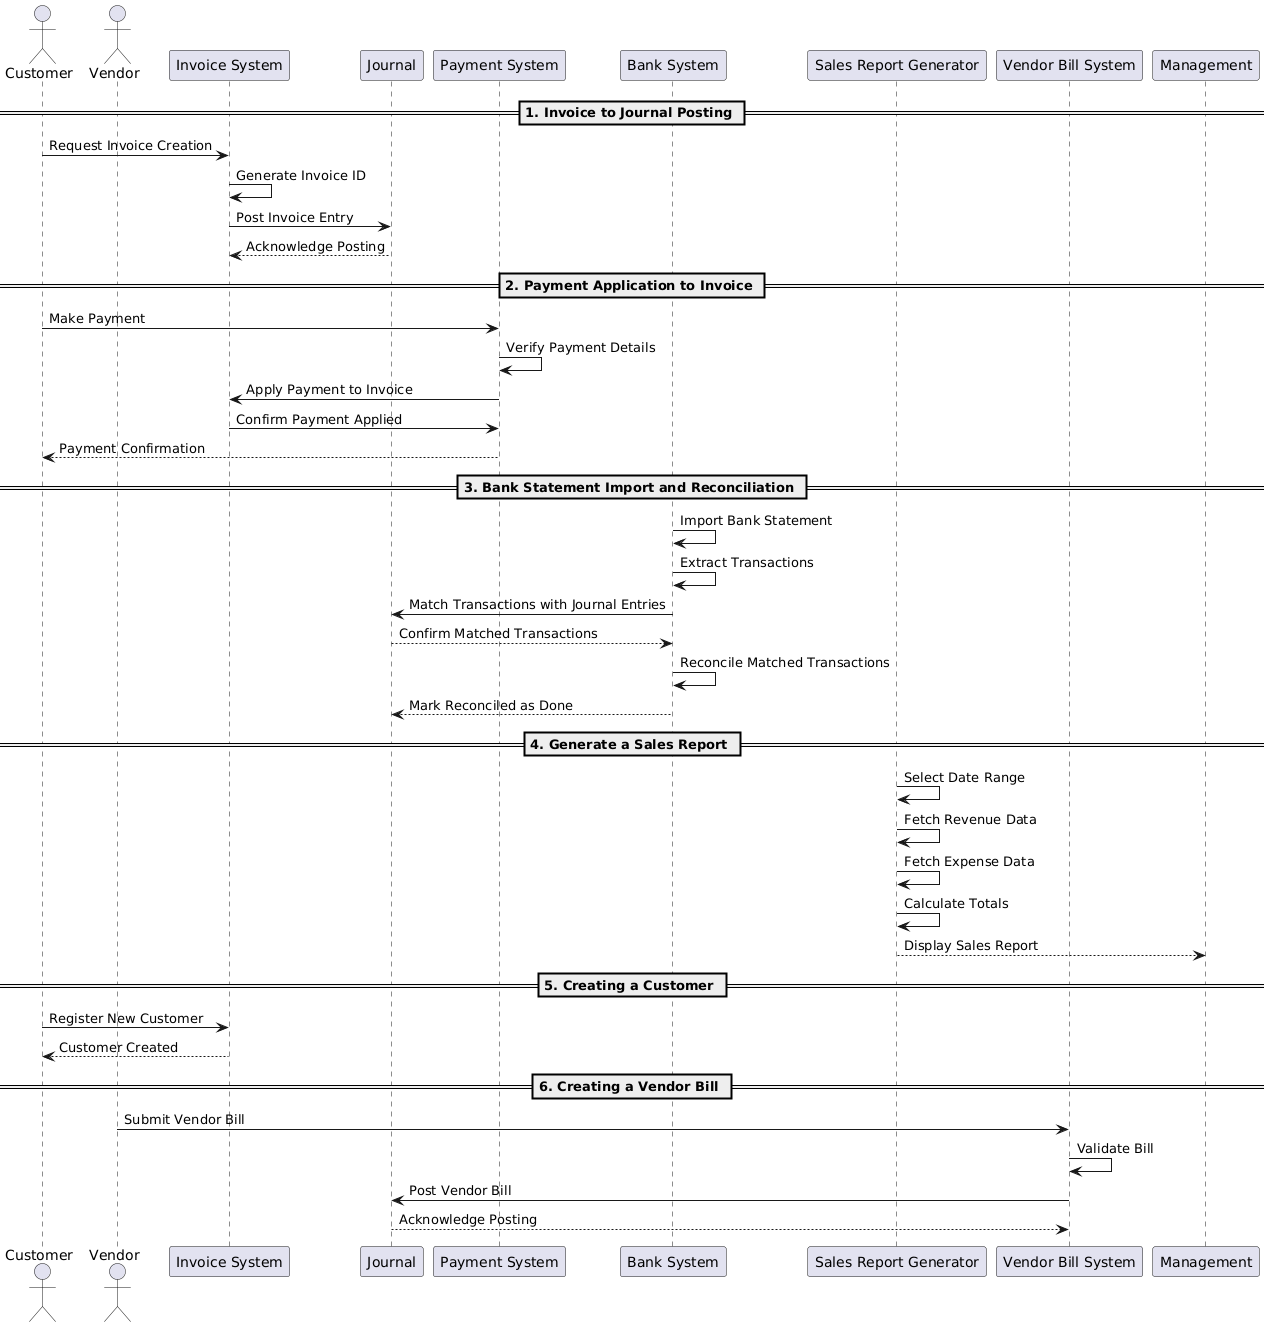
\includegraphics[width=\linewidth]{diagram/sequence_accounting_diagram.png}
\end{center}

\noindent\textbf{Overview of key processes:}
\begin{enumerate}
    \item \textbf{Invoice to Journal Posting:}
    
    -Customer asks system to generate invoice from the Invoice System.

	-System generates invoice ID, posts invoice to Journal, and receives acknowledgment.

    \item \textbf{Payment Application to Invoice:}
    
    -Customer applies payment via the Payment System.

	-Payment details are verified, applied to invoice, and payment confirmation is signaled.

    \item \textbf{Bank Statement Import \& Reconciliation:}
    
    -The Bank System imports bank statements, extracts and reconciles transactions with journal entries.

	-Confirmed and reconciled matched transactions, and status is done.

    \item \textbf{Generating a Sales Report:}
    
    -The system facilitates choosing a date range, fetching revenue and expenses, summing totals, and returning the sales report.

    \item \textbf{Creating a Customer:}
    
    -New customers are inserted via the system, and creating a customer is triggered.

    \item \textbf{Creating a Vendor Bill:}
    
    -Vendors submit bills, which are validated and posted by the Vendor Bill System, with acknowledgment.

\end{enumerate}

\noindent\textbf{Class Diagram}
\begin{center}
    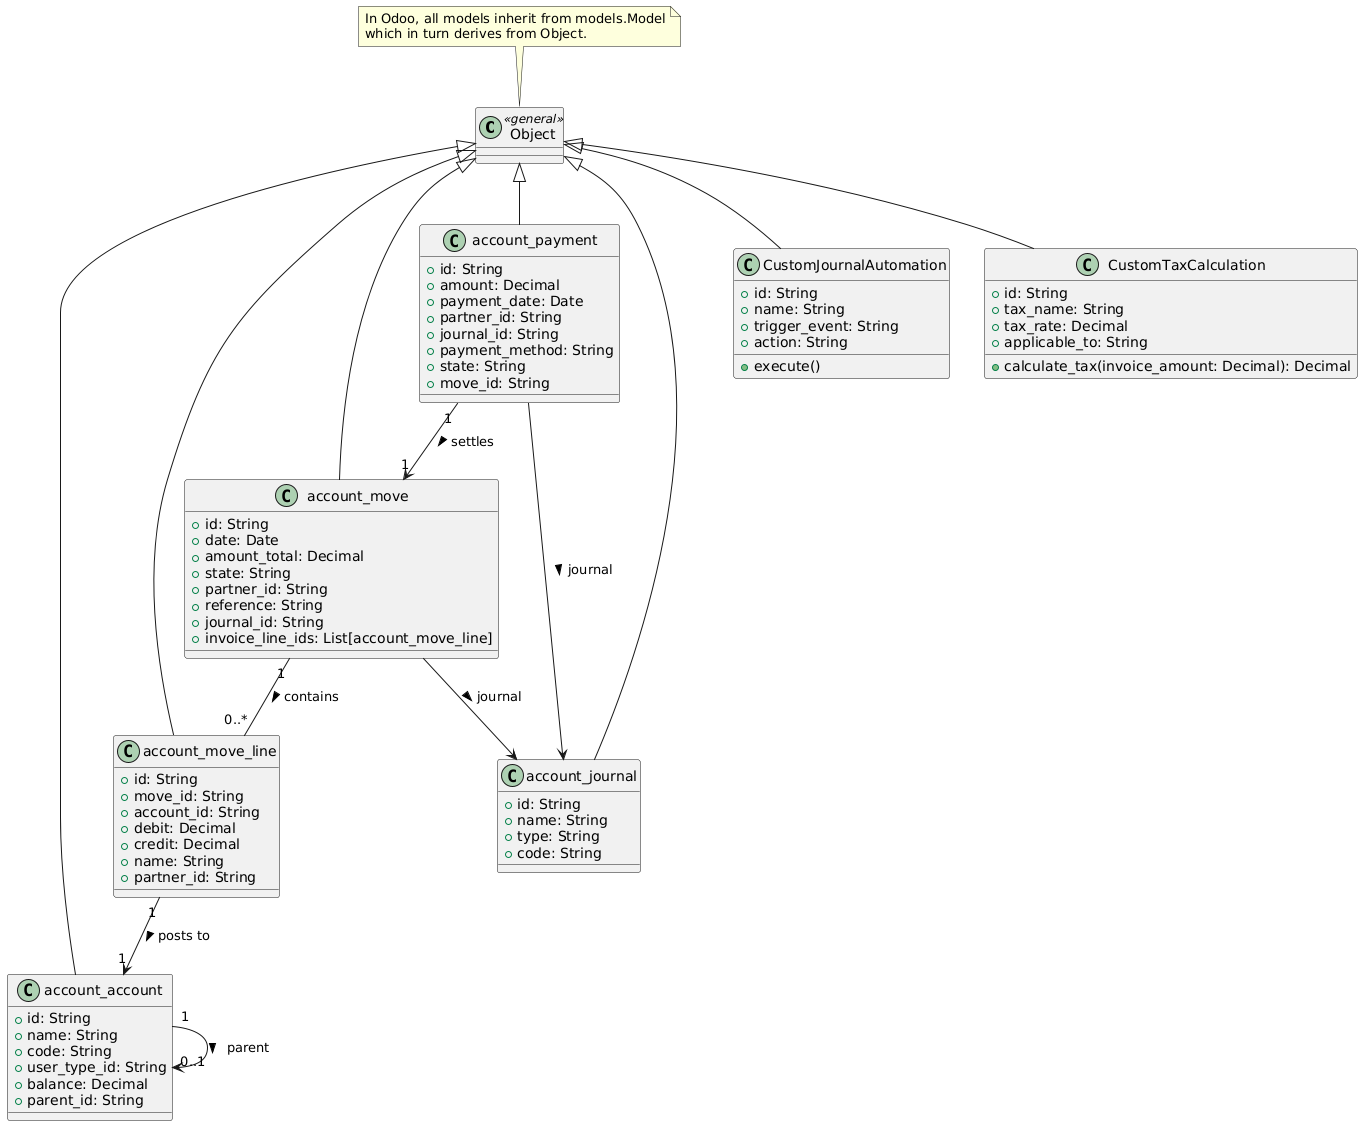
\includegraphics[width=\linewidth]{diagram/class_diagram_account.png}
\end{center}

\noindent This is a class diagram illustrating the static structure and relations of a financial accounting system that has been designed with UML.
\medskip

\noindent\textbf{Key Components:}

\noindent\textbf{Object (Base Class):}
\noindent Serves as the superclass to which other classes are extended, as indicated by the note referring to Odoo's model inheritance.

\noindent\textbf{Classes and Attributes:}
\begin{itemize}
    \item account\_move: Employed to represent invoice headers with attributes like id, date, amount\_total, state, partner\_id, reference, and a list of associated invoice lines (invoice\_line\_ids).
    \item account\_move\_line: Represents individual invoice line items against an invoice (move\_id), with information like account\_id, debit, credit, name, and partner\_id.
    \item account\_journal: Represents journal entries containing id, name, type, and code.
    \item account\_payment: Contains payments, related to invoices, with characteristics like id, amount, payment\_date, partner\_id, journal\_id, payment\_method, state, and the related move\_id.
    \item account\_account: Represents chart of accounts, with identifiers, name, code, user\_type, balance, and parent account relation.
    \item CustomJournalAutomation: Custom class for journal entry automation, with id, name, trigger\_event, action; and an execute() method.
    \item CustomTaxCalculation: Class for tax information, with fields for the tax name, rate, applicable-to info, and a calculate\_tax() method to compute taxes on invoice amounts.
\end{itemize}
\medskip

\noindent\textbf{Relationships:}

\noindent\textbf{Inheritance:} A number of classes inherit from Object, i.e., they are models in a hierarchy.

\noindent\textbf{Associations:}
\begin{itemize}
    \item account\_move has multiple account\_move\_line items (invoice\_line\_ids).
    \item account\_move is associated with account\_journal.
    \item account\_payment is applied to account\_move.
    \item account\_move\_line posts to account\_account.
    \item CustomJournalAutomation is associated with account\_move.
    \item CustomTaxCalculation is used on invoices (account\_move).
\end{itemize}
\medskip

\noindent\textbf{Overall:}

This UML class diagram defines the key entities involved in invoice processing, payments, accounting, and custom automation/tax calculation in an enterprise finance system, their attributes, and how they relate to each other.
\bigskip

\noindent\textbf{Component Diagram}
\begin{center}
    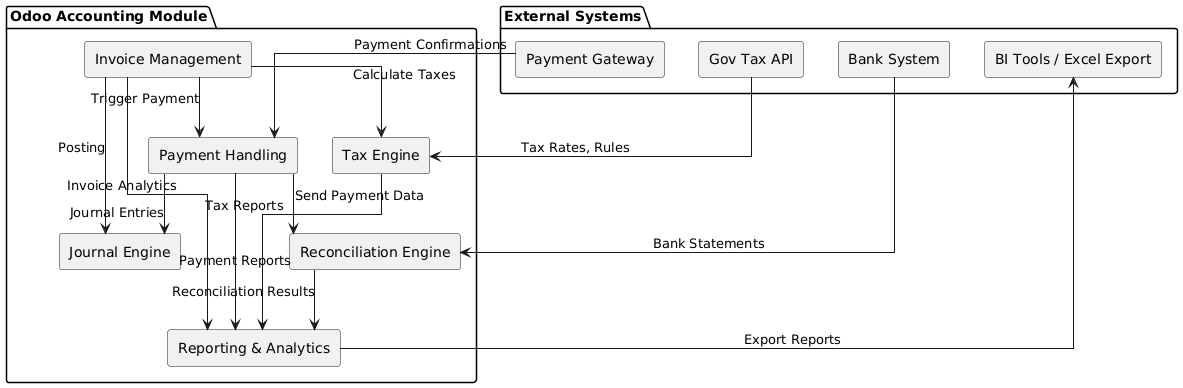
\includegraphics[width=\linewidth]{diagram/component_diagram.png}
\end{center}

\noindent The component diagram of the Odoo Accounting module provides a comprehensive view of the overall structure of the system, describing internal components and how they communicate with external systems. The module internally divides into distinct components such as Invoice Management, Payment Management, Reconciliation Engine, Reporting and Analytics, Tax Engine, and Journal Engine. Every module contains specialized duties, e.g., Invoice Management is in charge of invoice creation and tracking and the Tax Engine handles tax rule application and reporting. The modules communicate with each other; the Payment Handling system relies on the Invoice Management and Journal Engine modules, for example, to properly 
process and book financial transactions. Externally, the system integrates with third-party 
systems like Bank Systems (reconciliation), Payment Gateways (receipt and payout of 
payments), Government Tax APIs (tax reporting and compliance), and BI Tools or Excel 
(advanced reporting and analysis). The integrated and modular architecture allows the Odoo 
Accounting system to be extensible and solid, enabling seamless integration and efficient 
financial management.
\bigskip

\noindent\textbf{Deployment Diagram}
\begin{center}
    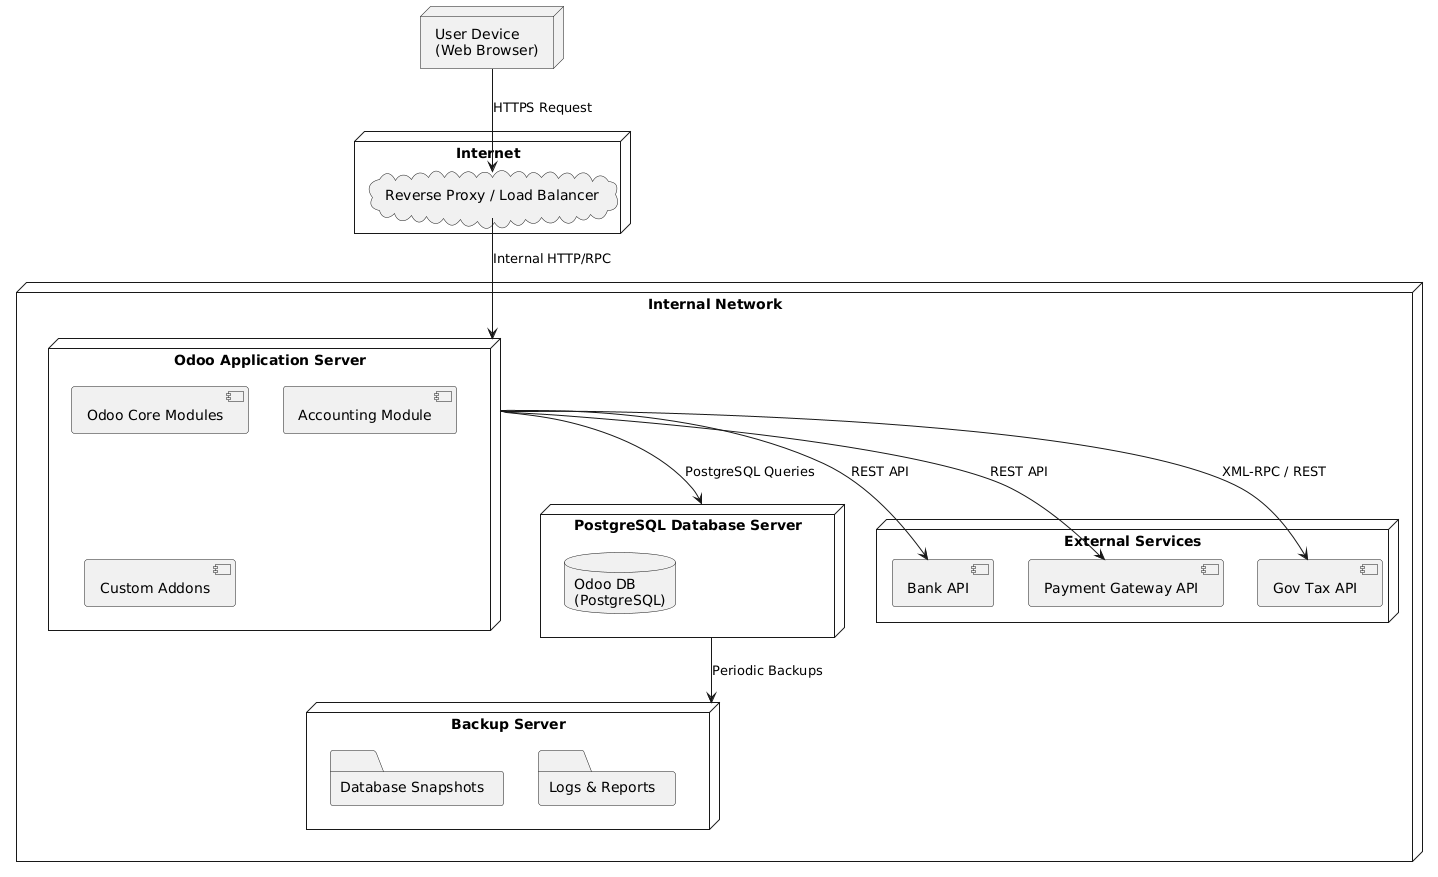
\includegraphics[width=\linewidth]{diagram/Deployment_Diagram.png}
\end{center}

\noindent This deployment diagram illustrates the physical structure of an Odoo system with emphasis on 
the Accounting Module. Users access the application through a web browser over the internet 
through a reverse proxy or load balancer to distribute traffic and terminate SSL. The Odoo 
Application Server hosts the base Odoo modules, including the Accounting Module and any 
addons developed custom. It interacts with a PostgreSQL Database Server that contains all 
transactional and config data.
\medskip

\noindent The Odoo software also integrates with various external services such as banking APIs, payment 
gateways, and government taxation systems to provide support for functionality such as 
automatic reconciliation, online payments, and regulatory reporting. The architecture also 
includes a backup server containing snapshots of the databases and significant logs at periodic 
intervals to ensure data security and recovery alternatives. The secure and modular deployment 
design facilitates scalability, external integration, and financial compliance operations.
\bigskip

\newpage
\noindent\textbf{Report Architecture Diagram}
\begin{center}
    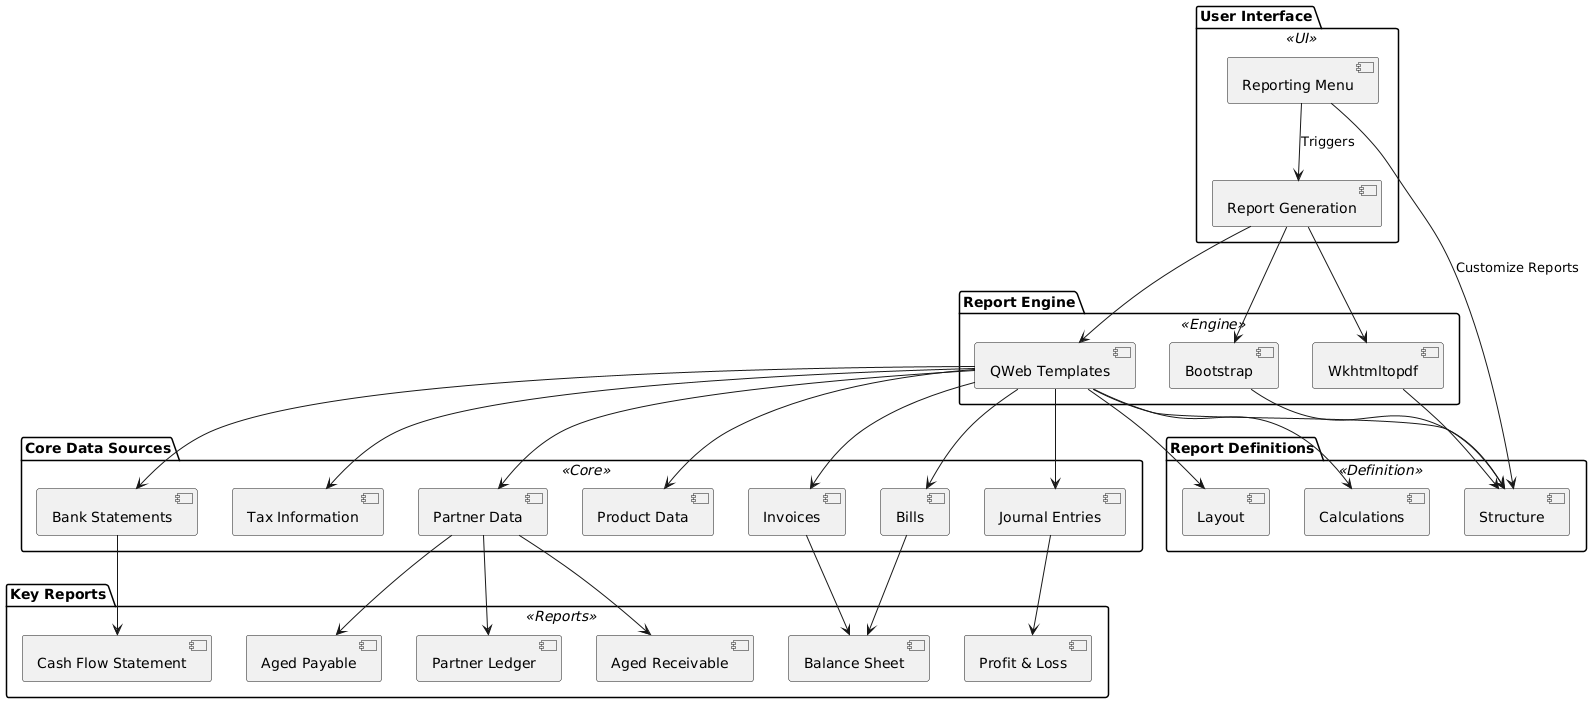
\includegraphics[width=\linewidth]{diagram/report_architecture.png}
\end{center}
\medskip

\noindent The system architecture of the Odoo reporting system for accounting and invoicing modules is 
presented in the diagram. The Data Sources form the core of the system and include key 
financial documents that are associated with invoices, bills, journal entries, bank statements, tax 
information, partner details, and product details. The Report Engine takes input from these data 
sources and utilizes reporting templates like QWeb, Bootstrap, and Wkhtmltopdf to generate 
reports in various formats. The user interaction is facilitated by the User Interface, where users 
launch the reporting menu, customize reports, and trigger report generation. The report 
generation revolves around the Report Definitions, where the structure, format, and calculations 
needed for every report are defined. The report engine then takes this information and produces 
the final reports, including key financial reports like the Balance Sheet, Profit \&Loss, Cash 
Flow Statement, and others. Overall, this architecture enables customized, data-based reporting 
with a logical evolution from data collection to final report generation.

\newpage
\noindent\textbf{Activity Diagram}

\begin{minipage}{0.45\textwidth}
    \centering
    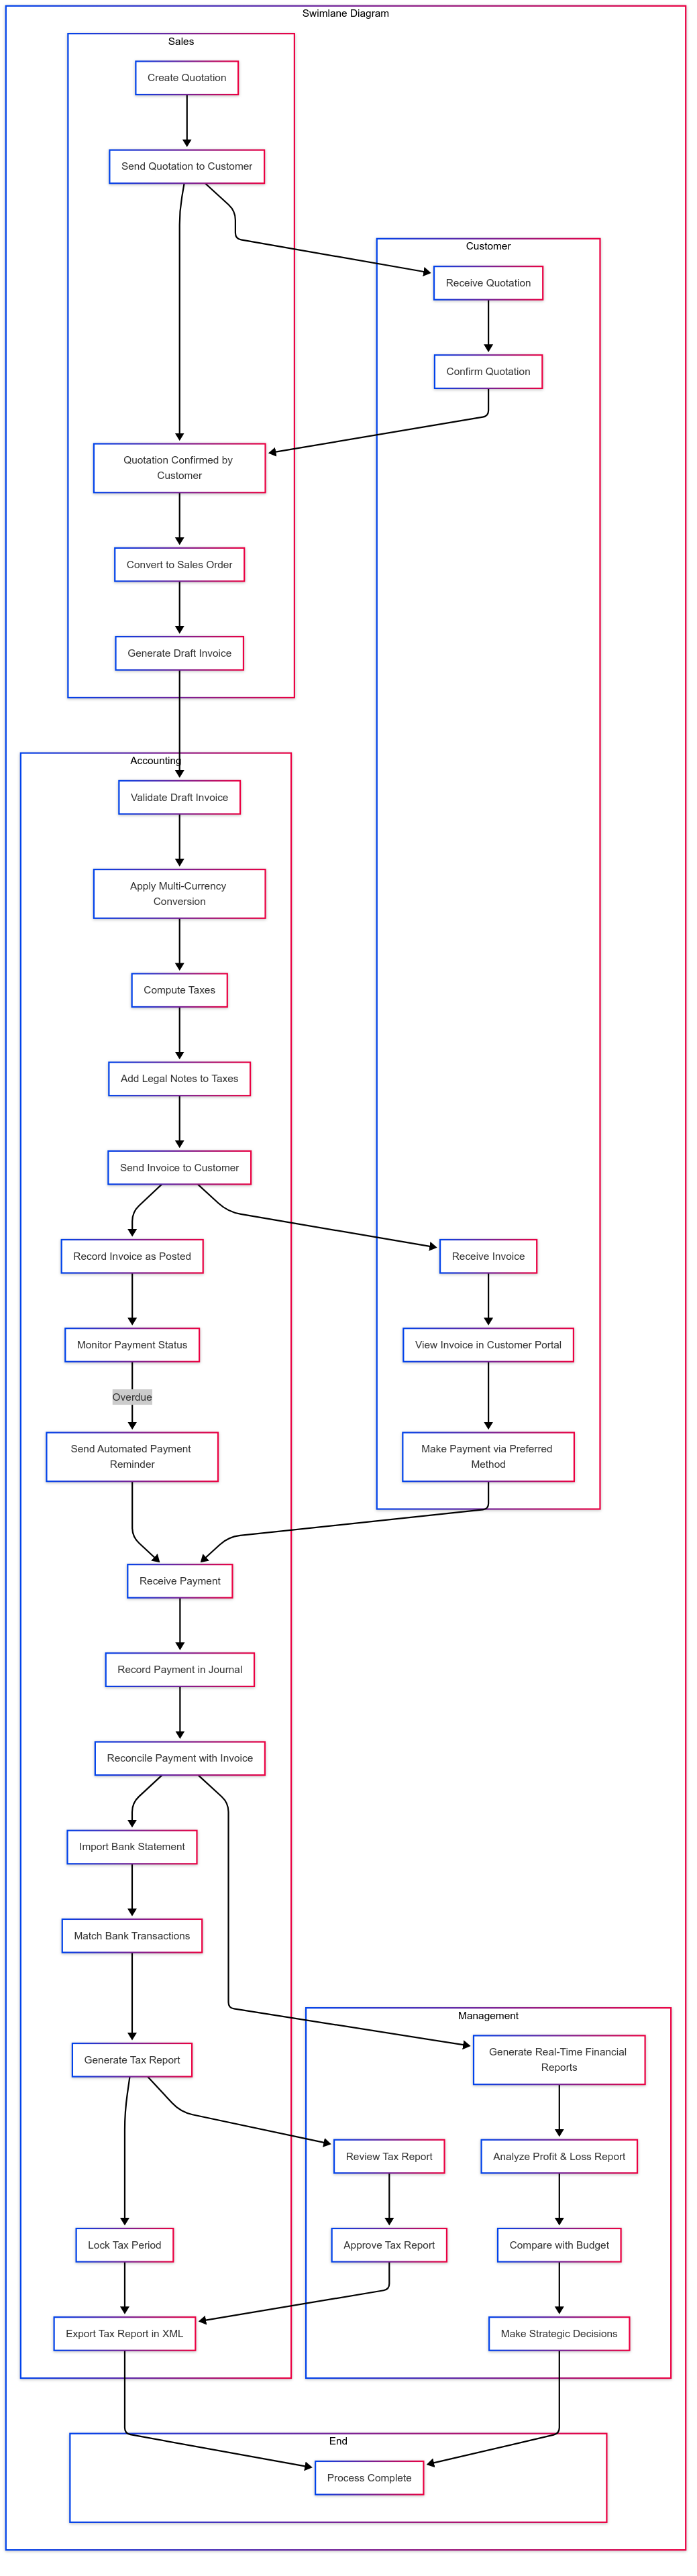
\includegraphics[width=\linewidth, height=0.8\textheight, keepaspectratio]{diagram/Swimlane.png}
\end{minipage}%
\hfill
\begin{minipage}{0.5\textwidth}
    The diagram illustrates the end-to-end accounting and billing process in Odoo 18, integrating the activities of various departments: Sales, Accounting, Customer, and Management. The process begins when the Sales department quotes a customer. The quote is then submitted to the customer for approval. Upon confirmation by the customer, the quote is converted into a sales order. Odoo 18 also generates an automatically created draft invoice based on this sales order (Web ID: 2, 8).
    \medskip

    At the Accounting step, the draft invoice is approved and validated by the accounting staff (Web ID: 2). If there is a foreign currency transaction, Odoo 18 refreshes with the latest exchange rate and records the base and foreign currencies (Web ID: 0, 18). Taxes are then calculated against the relevant country localization, accommodating price included or excluded, diverse tax rates, and partial exemptions (Web ID: 1). Legal remarks can also be added to specific taxes to assist with regulatory adherence (Web ID: 5). After this, the invoice is sent to the customer through their desired delivery method such as email or Peppol (Web ID: 4, 16), and its status is set to "Posted," posting journal entries automatically using double-entry bookkeeping (Web ID: 0, 16).
    \medskip

    Accounting then goes on to monitor the status of payment. If the payment is overdue, Odoo 18 triggers its dunning procedure, sending automatic reminders to the customer (Web ID: 3, 18). Upon acceptance of the payment, it is recorded as a journal entry (Web ID: 1) and matched against the corresponding invoice using Odoo's smart matching algorithm, which does 95% of the work automatically (Web ID: 1). Bank statements may be imported in various forms such as.OFX,.QIF, or.CSV through synchronization (Web ID: 1, 5), and transactions are reconciled with bills or invoices to 
    further minimize manual intervention (Web ID: 1, 18). A tax report is subsequently generated, 
    cash or accrual basis (Web ID: 0), the tax period is locked to prevent additional VAT-related 
    postings (Web ID: 0), and the report is exported to XML format for tax authority filing (Web ID: 
    0).
    \medskip
\end{minipage}
On the side of the Customer, they validate and accept the quotation, which triggers the creation 
of the sales order. On receiving approved invoice, customers can view and download it through 
Odoo's Customer Portal (Web ID: 1) and subsequently arrange for payment through their 
preferred medium such as SEPA or online gateway like Stripe (Web ID: 1, 4).
\medskip

\noindent Finally, Management reviews the tax report, signs it off for filing, and uses Odoo's real-time 
financial reporting features to generate vital reports such as the profit and loss statement (Web 
ID: 7, 18). They review financial performance and contrast it with budgeted (Web ID: 1), using 
these insights to inform strategic business decisions. The cycle ends when all the accounting and 
invoicing functions are finalized and closed.

\subsection{Useful Odoo Resources and Documentation links}
Here are some useful Odoo resources and links to documentation for finance:
\medskip

\noindent\textbf{General Finance Resources:}
\begin{itemize}
    \item \textbf{Finance:} This is the main landing page for Odoo's finance documentation, providing an overview of the various finance-related topics. 
    
    https://www.odoo.com/documentation/18.0/applications/finance.html

    \item \textbf{Accounting and Invoicing:}
    \begin{itemize}
        \item \textbf{Accounting and Invoicing:} This page describes the fundamental accounting features of Odoo, including invoicing, managing payments, and setting up your chart of accounts. 
        
        https://www.odoo.com/documentation/18.0/applications/finance/accounting.html

        \item \textbf{Customer Invoices:} Discover how to create, send, and manage customer invoices in Odoo. 
        
        https://www.odoo.com/documentation/18.0/applications/finance/accounting/customer\_invoices.html

        \item \textbf{Invoicing Processes:} This section explains how to automate customer invoice generation in Odoo, for example, from sales order, delivery order, and contract. 
        
        https://www.odoo.com/documentation/18.0/applications/finance/accounting/customer\_invoices/overview.html

        \item \textbf{Electronic Invoicing (EDI):} earn about electronic data interchange for business documents like invoices. 
        
        https://www.odoo.com/documentation/18.0/applications/finance/accounting/customer\_invoices/electronic\_invoicing.html

        \item \textbf{Odoo electronic invoicing in Austria:} Information about legally compliant e-invoicing solutions for Austria. 
        
        https://www.odoo.com/documentation/18.0/applications/finance/accounting/customer\_invoices/electronic\_invoicing/austria.html

        \item \textbf{Invoicing Method:} Explains various invoicing methods, for example, down payments, pro-forma invoices, and time and material-based invoicing. 
        
        https://www.odoo.com/documentation/18.0/applications/sales/sales/invoicing.html
	
        \item \textbf{Invoicing by time and materials:} Information on how to invoice customers by time and/or materials. 
        
        https://www.odoo.com/documentation/18.0/applications/sales/sales/invoicing/time\_materials.html
    \end{itemize}
    \item \textbf{Accounting Features and Configuration:}
    \begin{itemize}
        \item \textbf{Chart of Accounts:} This is the explanation of the chart of accounts, which is the list of all accounts used to record financial transactions. 
        
        https://www.odoo.com/documentation/18.0/applications/finance/accounting/get\_started/chart\_of\_accounts.html

        \item \textbf{Bank and Cash Accounts:} Learn how to manage your bank and cash accounts in Odoo. 
        
        https://www.odoo.com/documentation/18.0/applications/finance/accounting/bank.html

        \item \textbf{Bank Synchronization:} Find out how to synchronize Odoo with your bank to automatically import bank statements. 
        
        https://www.odoo.com/documentation/18.0/applications/finance/accounting/bank/bank\_synchronization.html

        \item \textbf{Loans Management:} This section describes how to manage loans taken by your company. 
        
        https://www.odoo.com/documentation/18.0/applications/finance/accounting/bank/loans.html

        \item \textbf{Online Payments:} Find out how to install and manage online payments in Odoo. 
        
        https://www.odoo.com/documentation/18.0/applications/finance/payment\_providers.html

        \item \textbf{Payments:} This section describes how payments can be linked to invoices or as standalone records. 
        
        https://www.odoo.com/documentation/18.0/applications/finance/accounting/payments.html
    \end{itemize}
    \item \textbf{Reporting:} 
    \begin{itemize}
        \item \textbf{Reporting:} This chapter has details about Odoo's various financial reports, such as the Balance Sheet, Profit and Loss account, and Cash Flow statement.
        
        https://www.odoo.com/documentation/18.0/applications/finance/accounting/reporting.html

        \item \textbf{Year-End Closing:} Learn about the year-end closing process in Odoo.
        
        https://www.odoo.com/documentation/18.0/applications/finance/accounting/reporting/year\_end.html
    \end{itemize}

    \item \textbf{Getting Started:}
    \begin{itemize}
        \item \textbf{Get Started:} It takes you through the Odoo Accounting initial setup.
        
        https://www.odoo.com/documentation/18.0/applications/finance/accounting/get\_started.html
    \end{itemize}
\end{itemize}

\end{document}
